% ------------------------------------------------------------------------
% ------------------------------------------------------------------------
% abnTeX2: Modelo de Trabalho Academico (tese de doutorado, dissertacao de
% mestrado e trabalhos monograficos em geral) em conformidade com 
% ABNT NBR 14724:2011: Informacao e documentacao - Trabalhos academicos -
% Apresentacao
% ------------------------------------------------------------------------
% ------------------------------------------------------------------------

% ------------------------------------------------------------------------
% ------------------------------------------------------------------------
% abnTeX2: Modelo de Trabalho Academico (tese de doutorado, dissertacao de
% mestrado e trabalhos monograficos em geral) em conformidade com 
% ABNT NBR 14724:2011: Informacao e documentacao - Trabalhos academicos -
% Apresentacao
% ------------------------------------------------------------------------
% ------------------------------------------------------------------------

\documentclass[
	% -- opções da classe memoir --
	12pt,				% tamanho da fonte
	openright,			% capítulos começam em pág ímpar (insere página vazia caso preciso)
	twoside,			% para impressão em verso e anverso. Oposto a oneside
	a4paper,			% tamanho do papel. 
	% -- opções da classe abntex2 --
	%chapter=TITLE,		% títulos de capítulos convertidos em letras maiúsculas
	%section=TITLE,		% títulos de seções convertidos em letras maiúsculas
	%subsection=TITLE,	% títulos de subseções convertidos em letras maiúsculas
	%subsubsection=TITLE,% títulos de subsubseções convertidos em letras maiúsculas
	% -- opções do pacote babel --
	english,			% idioma adicional para hifenização
	french,				% idioma adicional para hifenização
	spanish,			% idioma adicional para hifenização
	brazil				% o último idioma é o principal do documento
	]{abntex2}

	% ---
	% Pacotes básicos 
	% ---
	\usepackage{lmodern}			% Usa a fonte Latin Modern			
	\usepackage[T1]{fontenc}		% Selecao de codigos de fonte.
	\usepackage[utf8]{inputenc}		% Codificacao do documento (conversão automática dos acentos)
	\usepackage{lastpage}			% Usado pela Ficha catalográfica
	\usepackage{indentfirst}		% Indenta o primeiro parágrafo de cada seção.
	\usepackage{color}				% Controle das cores
	\usepackage{graphicx}			% Inclusão de gráficos
	\usepackage{microtype} 			% para melhorias de justificação
	\usepackage{epsfig,psfrag,amsmath,tabularx} % para figuras eps e simbolos matematicos
% ---

\usepackage{backnaur}
\usepackage{chngcntr}
\usepackage{pgf}
\usepackage{tikz}
\usetikzlibrary{arrows, automata, shapes}
\usetikzlibrary{positioning}
\usetikzlibrary{arrows.meta}
\tikzset{>={Latex[width=3mm,length=3mm]}}
\usepackage{makecell}
\usetikzlibrary{calc}

\usepackage[final]{pdfpages}
\usepackage{pgf-umlsd}
% -----------------
% Configurações adicionais

\usepackage{float}

\newcommand{\srcstyle}[1]{\ttfamily\textbf{#1}\rmfamily}

\newcommand{\mychaptermark}[1]{
	\markboth{#1}{}}

\usepackage{xcolor}
\definecolor{black}{RGB}{0,0,0}
\newcommand{\verify}[1]{\textcolor{red}{#1}}

\newlength{\MaxSizeOfLineNumbers}%
\settowidth{\MaxSizeOfLineNumbers}{99}% Adjust to maximum number of lines
\addtolength{\MaxSizeOfLineNumbers}{1ex}%
% Configurando layout para mostrar codigos Java

\usepackage{listings}
\lstset{
	language=Java,
	keywordstyle=\color{black},
	stringstyle=\color{black},
	commentstyle=\color{black},
	morecomment=[s][\color{black}]{/**}{*/},
	extendedchars=true,
	showspaces=false,
	showstringspaces=false,
	numbers=left,
	numberstyle=\tiny,
	breaklines=true,
	backgroundcolor=\color{white},
	breakautoindent=true,
	captionpos=b,
	xleftmargin=\MaxSizeOfLineNumbers,
	tabsize=2,
	frame=single,
	basicstyle=\linespread{0.8}\fontsize{10}{\baselineskip}\selectfont\ttfamily,
	framexleftmargin=0pt,
	framexrightmargin=-4pt,
	framextopmargin=2pt,
	framexbottommargin=2pt,
	aboveskip=25pt,
	abovecaptionskip=15pt,
	belowskip=15pt
}

\usepackage[utf8]{inputenc}
%\usepackage{graphicx}

\setlength{\FrameSep}{1pt}

% corrige paragrafo que termina com linha com uma palavra 
\setlength\parfillskip{0pt plus .75\textwidth}
\setlength\emergencystretch{1pt}

\usepackage{amsmath,mathpazo}

%------------------
\usepackage{etoolbox}
\makeatletter
%\patchcmd{\@caption}{\csname the#1\endcsname}{\csname fnum@#1\endcsname:}{}{}
\renewcommand*\l@figure{\@dottedtocline{1}{1.5em}{2.5em}} % default for 3rd arg: 2.3em
%\let\l@table\l@figure % as in article.cls
\makeatother
% ---
% Pacotes de citações
% ---
\usepackage[brazilian,hyperpageref]{backref}	 % Paginas com as citações na bibl
\usepackage[alf]{abntex2cite}					 % Citações padrão ABNT

% --- 
% CONFIGURAÇÕES DE PACOTES 
% --- 

% ---
% Configuracoes do pacote backref
% Usado sem a opcao hyperpageref de backref
\renewcommand{\backrefpagesname}{Citado na(s) página(s):~}
% Texto padrao antes do numero das paginas
\renewcommand{\backref}{}
% Define os textos da citacao
\renewcommand*{\backrefalt}[4]{
	\ifcase #1 %
		Nenhuma citação no texto.%
	\or
		Citado na página #2.%
	\else
		Citado #1 vezes nas páginas #2.%
	\fi}%
% ---

% ---
% Pacotes definidos pelo autor
% ---
\input{macros}		% arquivo com possiveis macros definidas pelo autor
% ---

% ---
% Informacoes de dados para CAPA e FOLHA DE ROSTO
% ---
\titulo{Replicação Orientada a Metaprogramação} % Replicação Metaprogramada
\autor{Fellipe Augusto Ugliara}
\local{Sorocaba, SP}
\data{12 de Junho de 2018}
\orientador{Prof. Dr. José de Oliveira Guimarães}
\coorientador{Prof. Dr. Gustavo Maciel Dias Vieira}
\instituicao{%
  Universidade Federal de São Carlos -- UFSCar
  \par
  Centro de Ciências em Gestão e Tecnologia -- CCGT
  \par
  Programa de Pós-Graduação em Ciência da Computação -- PPGCC-So}
\tipotrabalho{Dissertação (Mestrado)}
% O preambulo deve conter o tipo do trabalho, o objetivo, 
% o nome da instituicao e a Area de concentracao 
\preambulo{Dissertação de mestrado apresentada ao Programa de Pós-Graduação em Ciência da Computação (PPGCC-So) da Universidade Federal de São Carlos como parte dos requisitos exigidos para a obtenção do título de Mestre em Ciência da Computação. Linha de pesquisa: Computação Científica e Inteligência Computacional.}
% ---

% ---
% Configuracoes de aparencia do PDF final

% alterando o aspecto da cor azul
\definecolor{blue}{RGB}{41,5,195}

% informacoes do PDF
\makeatletter
\hypersetup{
     	%pagebackref=true,
		pdftitle={\@title}, 
		pdfauthor={\@author},
    	pdfsubject={\imprimirpreambulo},
	    pdfcreator={LaTeX with abnTeX2},
		pdfkeywords={abnt}{latex}{abntex}{abntex2}{trabalho acadêmico}, 
		colorlinks=true,       		% false: boxed links; true: colored links
    	linkcolor=blue,          	% color of internal links
    	citecolor=blue,        		% color of links to bibliography
    	filecolor=magenta,      		% color of file links
		urlcolor=blue,
        bookmarksdepth=4
}
\makeatother
% --- 

% --- 
% Espacamentos entre linhas e paragrafos 
% --- 

% O tamanho do paragrafo é dado por:
\setlength{\parindent}{1.3cm}

% Controle do espaçamento entre um parágrafo e outro:
\setlength{\parskip}{0.2cm}  % tente também \onelineskip

% ---
% compila o indice
% ---
\makeindex
% ---

% ----
% Inicio da dissertacao
% ----
\begin{document}

% Retira espaco extra obsoleto entre as frases.
\frenchspacing


% ----------------------------------------------------------
% ELEMENTOS PRE-TEXTUAIS
% ----------------------------------------------------------
% \pretextual

% ---
% Capa
% ---
\imprimircapa
% ---

% ---
% Folha de rosto
% (o * indica que havera a ficha bibliografica)
% ---
\imprimirfolhaderosto*
% ---

% ---
% Inserir a ficha bibliografica
% ---
\begin{tikzpicture}[remember picture,overlay]
  \node at (current page.center) {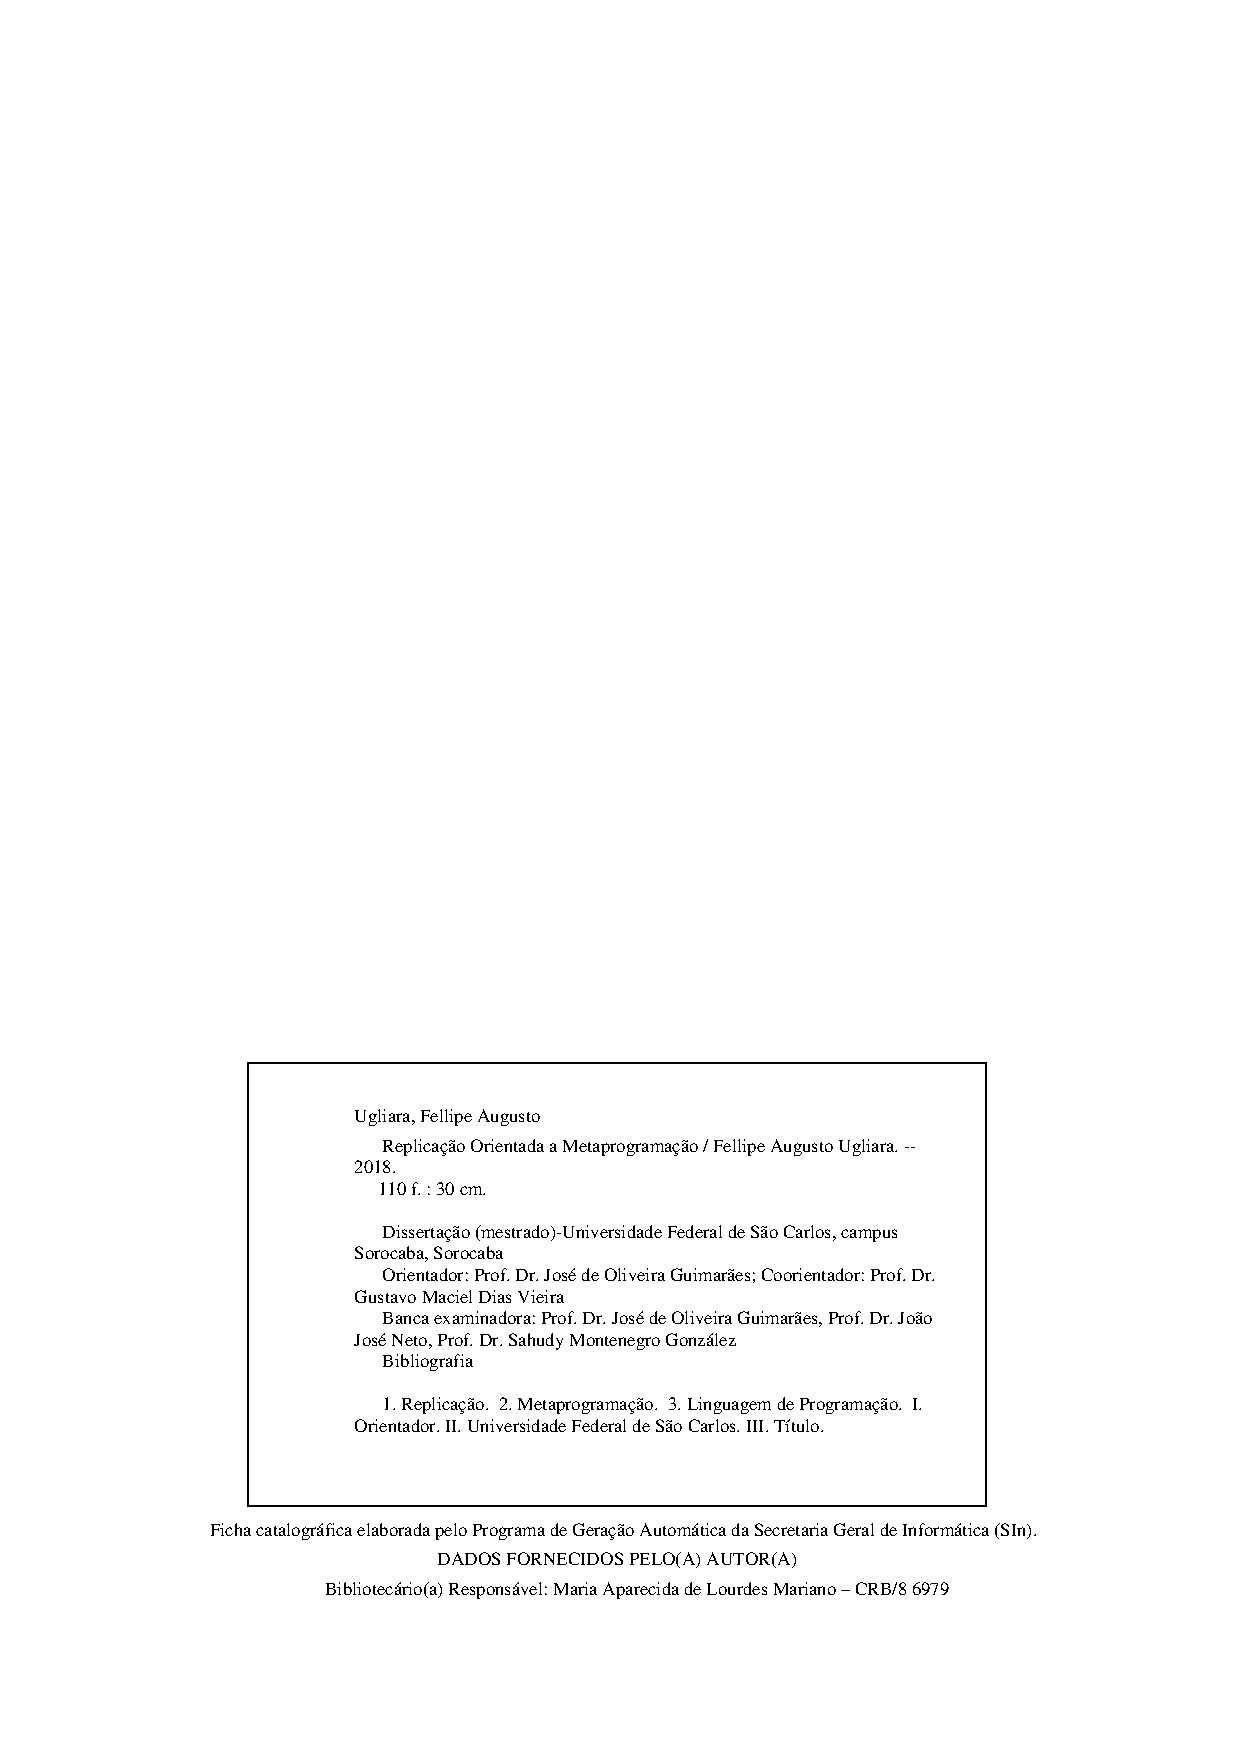
\includegraphics[page=1]{conteudo/pdfs/fichacatalografica.pdf}};
\end{tikzpicture}

\newpage

% ---

% ---
% Inserir folha de aprovacao
% ---
% Este é um exemplo de Folha de aprovacao, elemento obrigatorio da NBR
% 14724/2011 (secao 4.2.1.3). Voce pode utilizar este modelo ate a aprovacao
% do trabalho.

\begin{tikzpicture}[remember picture,overlay]
  \node at (current page.center) {\includegraphics[page=1]{conteudo/pdfs/aprovacaofellipe.pdf}};
\end{tikzpicture}

\begin{folhadeaprovacao}
\vspace*{\fill} 
\end{folhadeaprovacao}
% ---

% ---
% Dedicatoria
% ---
%======================================== Dedicatoria =========================================
\begin{dedicatoria}
   \vspace*{\fill}
   \centering
   \noindent
   \textit{ Dedico essa pesquisa às traças que fizerem bom uso do papel, \\
   e a cada leitor que a tirar da gaveta.}
   \vspace*{\fill}
\end{dedicatoria}
%==============================================================================================

% ---

% ---
% Agradecimentos
% ---
%======================================= Agradecimentos =======================================
\begin{agradecimentos}

	\noindent Agradeço,\\[2mm]
	a Katia Ruriko Muramatsu por ser compreensiva e ajudar com inúmeras revisões.\\[2mm]
	a Ruriko Tasaki Muramatsu pelos almoços de domingo que não ajudei a preparar.\\[2mm]
	ao Bruno Henrique Ugliara pelas revisões e pelo apoio positivo a cada etapa completada.\\[2mm]
	ao Oswaldo Toshio Muramatsu pelas conversas ao final dos domingos de trabalho.\\[2mm]
	ao Nahim Alves de Souza por explicar as etapas burocráticas e ajudar com o \LaTeX.\\[2mm]
	ao Gustavo Marcello pela revisão técnica e pela paciência em escutar cada ideia.\\[2mm]
	a Ana Ugliara e ao Milton Ugliara por sempre me lembrarem de seguir aprendendo.\\[2mm]
	a Pretinha por cada latido que me ajudou a continuar acordado escrevendo.
\end{agradecimentos}
%==============================================================================================

% ---

% ---
% Epigrafe
% ---
%======================================== Epigrafe ===================================
\begin{epigrafe}
    \vspace*{\fill}
	\begin{flushright}
		\textit{``A linguagem fez-se para que nos sirvamos dela, \\
		não para que a sirvamos a ela.'' \\
		(A Língua Portuguesa, Fernando Pessoa)}
	\end{flushright}
\end{epigrafe}
%==============================================================================================


% ---

% ---
% RESUMOS
% ---
%================================= Resumo e Abstract ========================================
\setlength{\absparsep}{18pt} % ajusta o espaçamento dos paragrafos do resumo 
                     
% --- 
% resumo em português
% --- 
\begin{resumo}
\setlength\parfillskip{0pt plus .75\textwidth}
\setlength\emergencystretch{1pt}
O objetivo dessa pesquisa é mostrar como aplicações distribuídas, coesas e pouco acopladas podem ser desenvolvidas. A proposta é usar técnicas de metaprogramação em compilação para automatizar parte do desenvolvimento do código-fonte das aplicações e inspecionar esse código-fonte à procura de inconsistências. Para isso foi usado Treplica e Cyan. Treplica fornece uma estrutura para o desenvolvimento de aplicações distribuídas, enquanto a linguagem de programação Cyan provê suporte à metaprogramação. Esses recursos permitiram a criação de componentes que podem ser usados para desenvolver aplicações replicadas. Nessa pesquisa foi possível aplicar metaprogramação para automatizar etapas do desenvolvimento dessas aplicações, tornando o código-fonte da replicação melhor isolado do restante da aplicação. A verificação desse código-fonte na busca de inconsistências também pode ser demonstrada. Essa pesquisa não tem a pretensão de tratar todas as possibilidades de automatização do desenvolvimento do código-fonte replicado, e também não pretende tratar todas as verificações necessárias à replicação. O objetivo é mostrar que, usando metaprogramação em compilação, é possível automatizar o desenvolvimento e a inspeção de código-fonte das aplicações de modo geral.

\textbf{Palavras-chaves}: Replicação. Metaprogramação. Linguagens de Programação.

\end{resumo}
% --- 

\begin{resumo}[Abstract]
 \begin{otherlanguage*}{english}

The objective of this research is to show how distributed, cohesive and coupled applications can be developed. The proposal is to use metaprogramming technics in compilation to automate part of the applications source code development, and to inspect the source code to find inconsistencies. For this purpose Treplica and Cyan were used. Treplica provides a structure to the distributed applications development, while Cyan provides the support to metaprogramming. These resources allowed the components creation, which can be used to develop replicated applications. In this research it was possible to apply metaprogramming to automate developmento steps of these applications, making the source code of replication better isolated from the rest of the application. The verification of this source code to find inconsistencies can also be made. This research does not intend to solve all automation possibilities of the replicated source code development, and it does not intend to solve all necessary verifications to the replication either. The objective of this research is to show that, using metaprogramming, it is possible to automate the development and the inspection of the applications source code in general.   

\textbf{Keywords}: Replication. Metaprogramming. Programming Languages.

 \end{otherlanguage*}
\end{resumo}
% --- 

%===========================================================================================

% ---


%=============================== lista de figuras ==========================
\pdfbookmark[0]{\listfigurename}{lof}
\listoffigures*
\counterwithout{figure}{chapter}
\cleardoublepage

%=============================== codigo fonte ==========================
\renewcommand{\lstlistingname}{Código-Fonte}% Listing -> Algorithm
\renewcommand{\lstlistlistingname}{Lista de Códigos-Fonte}
\lstlistoflistings
\counterwithout{lstlisting}{chapter}
\cleardoublepage

%=============================== lista de tabelas ==========================
%\pdfbookmark[0]{\listtablename}{lot}
%\listoftables*
%\cleardoublepage


%====================== lista de abreviaturas e siglas =====================
%\input{conteudo/7-abreviaturas.tex}


%============================ lista de simbolos ============================
%\input{conteudo/8-simbolos.tex}


%=============================== sumario =============================================

\pdfbookmark[0]{\contentsname}{toc}
\tableofcontents*
\addtocontents{toc}{\vspace{-15.0pt}\small}
\cleardoublepage


% ----------------------------------------------------------
% AQUI INICIA OS ELEMENTOS DO TEXTO
% ----------------------------------------------------------
\textual

% ----------------------------------------------------------
% Capitulos
% 
% . Introdução
% .. Do problema e da pesquisa
% . Revisão, Bibliografica
% .. Treplica, Replicação Ativa
% .. Cyan, Metaobjetos
% ... Paradoxo da auto referencia
% ... Nemerle, Xtend, Groovy, Scala
% ... Definir Protocolo de Metaobjetos
% .. Trabalhos Relacionados
% . Pesquisa
% .. Iniciar com o Artigo
% . Estudo de Caso
% .. Demo Explicação
% . Conclusão
% . Referencias
%
%
% ----------------------------------------------------------

\setcounter{page}{1}

\chapter*{Introdução}\label{cap:introducao}
\addcontentsline{toc}{chapter}{Introdução}
\mychaptermark{Introdução}

Quem, em computação, nunca ouviu a frase - "use essa linguagem que vai ser mais fácil de implementar esse algoritmo". Se comparada à visão teórica de computação, essa afirmação pode parecer sem fundamento, afinal todas as linguagens que são Turing-completo~\cite{sipser2006introduction} permitem escrever os mesmos algoritmos e todas elas têm a mesma capacidade de representação. Também temos a tese de Church-Turing definindo que se uma função pode ser implementada por uma linguagem de programação, todas as demais linguagens de programação também podem implementar a mesma função~\cite{copeland2007church}. Então como pode ser melhor usar uma linguagem do que outra para implementar um determinado algoritmo, se as linguagens modernas são todas Turing-completas?

A escolha da linguagem é uma questão de estilo e da adaptação dela ao contexto do algoritmo implementado. Quanto mais próximas forem as abstrações fornecidas pelas linguagens dos algoritmos implementados com elas, menos complexas serão essas implementações~\cite{fowler2010domain}. Isso é motivação suficiente para o projeto contínuo de novas linguagens e para o aperfeiçoamento das linguagens existentes. Para flexibilizar essas adaptações aos domínios de aplicação, as linguagens modernas têm incorporado conceitos que permitem definir nos programas não somente como será a sua execução, mas também como será sua compilação e interpretação. Isso possibilita adaptar a compilação e interpretação para atender melhor as necessidades de cada aplicação.

Os compiladores e interpretadores têm geralmente etapas de execução definidas e únicas para qualquer aplicação que será compilada ou interpretada. Essas etapas podem, em determinados casos, tornar o desenvolvimento de uma aplicação mais complexo por conta das características inerentes a elas. As linguagens que têm incorporado funcionalidades para permitir aos programas redefinir, remover e adicionar novos comportamentos às etapas de compilação e interpretação, acabam por tornar o desenvolvimento dos programas menos complexo. Isso acontece porque os algoritmos que eram amarrados a comportamentos fixos de compilação e interpretação, agora podem adaptar etapas para que sejam mais adequadas a eles.

Não é novidade permitir que etapas fixas sejam adaptadas, esse é o caminho convencional de muitos conceitos em computação. Um paralelo pode ser feito com as bibliotecas de computação gráfica~\cite{rost2009opengl}, no início elas tinham um fluxo de execução fixo que passou a ser adaptável conforme as bibliotecas evoluíam (\emph{Shading Language}). Com as linguagens de programação não é diferente, no início elas tinham compiladores e interpretadores com etapas fixas e com o tempo passaram a ser mais flexíveis. Em ambos os casos foram criados mecanismos que permitiram usar as bibliotecas gráficas e as linguagens de programação para interagir com características vinculadas a elas próprias. No domínio das linguagens de programação, essa mecânica é chamada de metaprogramação e permite que as linguagens de programação definam funcionalidades a respeito de sua própria compilação, interpretação e execução.

O conceito de metaprogramação não é utilizado em um único contexto, por isso a metaprogramação não possui somente uma definição. Ela pode ser apresentada de modo diferente dependendo do contexto em que estiver sendo utilizada~\cite{damavsevivcius2015taxonomy}. Nessa pesquisa estamos interessados na definição de metaprogramação em tempo de compilação e não trataremos as demais formas de metaprogramação. A metaprogramação em compilação permite definir comportamentos não convencionais que o compilador pode executar dependendo do código-fonte que estiver compilando.

Por exemplo, em compilação usando metaprogramação, é possível adicionar uma funcionalidade ao compilador, para que toda vez que ele encontre uma função que retorna um valor de algum tipo específico, ele adicione antes desse retorno uma chamada de função que verifique se o valor retornado passa por uma validação respeitando um predicado. A chamada de função que foi adicionada pode de modo similar ser feita usando orientação a aspectos, que permite localizar pontos do código-fonte e realizar chamadas de funções nesses locais~\cite{kiczales1997aspect}. Aplicações orientadas a aspectos usam desse tipo de implementação para separar os requisitos funcionais dos não funcionais e tornar o código-fonte melhor organizado. 

Nessa pesquisa mostramos como a metaprogramação pode ser utilizada para separar requisitos não funcionais de modo diferente do que é feito usando orientação a aspectos. Ao contrário da orientação a aspectos, a metaprogramação possibilita explorar o código-fonte de forma mais abrangente, o que torna possível separar os requisitos não funcionais e verificar se o código-fonte respeita restrições impostas por esses requisitos. Essa verificação é uma tarefa que usando orientação a aspectos é bem mais difícil de realizar.

Essa pesquisa não usou orientação a aspectos em momento algum. A associação entre essa pesquisa e a orientação a aspectos está no problema que ambas resolvem. Esse problema é a separação do código-fonte dos requisitos funcionais do código-fonte dos requisitos não funcionais~\cite{glinz2007non}.

O requisito não funcional de redundância pode ser implementado em diferentes aplicações sem estar relacionado ao comportamento principal de cada uma delas. Uma aplicação que atenda a esse requisito se mantém disponível aos usuários mesmo que algum tipo de falha ocorra durante sua execução~\cite{cachin2011introduction}. As aplicações não redundantes se comportam de forma diferente, uma falha provavelmente fará com que essas aplicações se tornem indisponíveis para o usuário. Esse requisito não funcional foi selecionado para demonstrar como a metaprogramação permite separar dele o resto do código-fonte. Nesse caso prático, a metaprogramação também é usada para verificar o código-fonte procurando por restrições impostas pelo requisito de redundância da replicação.

Para implementar as aplicações redundantes foi usado o conceito de replicação. Cada aplicação replicada executa em mais de uma instância, assim se alguma instância falhar e parar de executar as outras podem manter a aplicação executando. Novas instâncias da mesma aplicação podem ser executadas a qualquer momento para recuperar uma instância que falhou. O mecanismo de replicação torna as aplicações redundantes. Ele também requer que as aplicações sejam implementadas de modo determinista. Essa restrição associada à replicação é verificada usando metaprogramação para evitar que as aplicações apresentem comportamentos não deterministas durante sua execução.

O comportamento determinista é aquele que, associado a uma condição inicial, sempre produzirá o mesmo resultado quando executado~\cite{wiesmann2000understanding}. Caso as instâncias executem um comportamento não determinista, mesmo que elas iniciem a execução a partir da mesma condição inicial, elas poderão obter resultados diferentes, tornando-se assim inconsistentes.

A linguagem de programação foco dessa pesquisa é Cyan, por fornecer suporte à metaprogramação em tempo de compilação e permitir integrar código-fonte Java em código-fonte Cyan com facilidade~\cite{guimaraes2013cyan}. Em Cyan, a metaprogramação é feita em Java e consiste na implementação de classes que herdam classes do compilador de Cyan e que podem estender suas interfaces. Esses metaobjetos são compilados para serem usados pelo compilador de Cyan durante determinadas etapas da compilação das aplicações desenvolvidas em Cyan.

O \emph{framework} Treplica foi utilizado para implementar o conceito de replicação~\cite{vieira08a}, ele é originalmente desenvolvido em Java e nessa pesquisa foi integrado em Cyan por meio de uma biblioteca desenvolvida em Cyan. Essa biblioteca cria uma casca para o código-fonte Java de Treplica, facilitando a implementação de aplicações de Cyan que usam Treplica. A metaprogramação foi utilizada para separar a biblioteca Treplica do restante da aplicação Cyan e para verificar se o código-fonte da aplicação possui comportamento não determinista. Caso o compilador encontre algum trecho de código-fonte não determinista, ele substituirá esse trecho por um código determinista e se ele não souber realizar essa substituição, ele retornará um erro de compilação.

O uso da metaprogramação no contexto da replicação acaba por reduzir os problemas de não determinismo inerentes a esse tipo de aplicação. Permitindo separar com maior transparência o código-fonte que implementa o mecanismo de replicação do restante da aplicação, reduzindo assim a complexidade do desenvolvimento das aplicações replicadas.

Como resultado da pesquisa foi possível diminuir a complexidade das aplicações replicadas, devido ao uso de metaprogramação. Essa abordagem de utilizar metaprogramação para isolar o requisito não funcional de redundância e a verificação do código-fonte na busca de erros associados a esse requisito é uma solução que pode ser estendida a outros requisitos não funcionais. Isso permite que essa pesquisa possa ser generalizada para outros contextos onde seja necessário separar requisitos não funcionais e garantir que o código-fonte atenda a determinadas restrições de programação.

Nos Capítulos~\ref{cap:metaprog} e~\ref{cap:replicacao} são tratados os conceitos usados nessa pesquisa. A linguagem de programação Cyan e seus mecanismos de metaprogramação são abordados com base em exemplos práticos, e o \emph{framework} Treplica é mostrado por meio de uma aplicação implementada em Java.

O Capítulo~\ref{cap:pesquisa} mostra como o \emph{framework} Treplica foi incorporado à linguagem de programação Cyan e como a metaprogramação foi utilizada para separar a replicação do restante do código-fonte da aplicação. Uma explicação sobre o problema de não determinismo também é apresentada neste capítulo. Ele termina explicando a implementação dos metaobjetos de Cyan que permitem o uso de Treplica de modo padronizado e transparente. 

No Capítulo~\ref{cap:estudo} são apresentados dois casos de uso de aplicações replicadas que foram implementadas usando metaprogramação. O primeiro é um jogo de tabuleiro para dois jogadores que usa replicação para permitir que cada jogador mantenha uma instância replicada do tabuleiro. O segundo exemplo trata de como os metaobjetos ajudam a evitar que os programas replicados criados sejam inconsistentes. No Apêndice~\ref{apd:metaobjetos} estão os códigos-fonte dos metaobjetos de Cyan desenvolvidos durante a realização dessa pesquisa.
 
\chapter{Metaprogramação em Compilação}
\label{cap:metaprog}

O objetivo desse capítulo e introduzir o conceito de metaprogramação. Ele inicia definindo uma linguagem de programação com elementos de metaprogramação em compilação. Essa linguagem é usada para mostrar como esse conceito funciona isoladamente de uma linguagem de programação real, que possui maior complexidade.

O capítulo segue detalhando a metaprogramação em compilação e mostrando a linguagem de programação Cyan, que é a linguagem principal dessa pesquisa. As etapas de compilação em Cyan são tratados junto com seus metaobjetos. A linguagem Xtend aparece no final do capítulo para mostrar um modelo de metaprogramação em compilação diferente do mostrado em Cyan.

\section{Execução e Compilação de Programas}

As linguagem de programação são um método padronizado para passar instruções a um computador~\cite{dershem1995programming}. Elas são regras sintáticas e semânticas usadas para definir programas de computador~\cite{fischer1993anatomy}. A semântica e a sintaxe são relacionadas à linguagem de programação por perspectivas diferentes. A semântica é relacionada ao significado da linguagem enquanto a sintaxe é associada a estruturas ou padrões formais de como a linguagem expressa esse significado~\cite{chomsky1955logical}.

Pela perspectiva da sintaxe uma linguagem é formada por tokens e regras. Os tokens são as palavras e os símbolos que pertencem à linguagem e as regras são a definição de como esses tokens podem ser agrupados de modo válido. Os possíveis agrupamento de tokens de uma linguagem de programação são chamados de sentenças. Dentre todas as sentenças que podem ser construídas com um conjunto de tokens, as que pertencem à linguagem são as que atendem a suas regras de agrupamento.

O conjunto de tokens da linguagem pode ser representado por expressões regulares, elas podem ser usadas para definir os tokens na maioria das linguagens de programação. As regras da sintaxe podem ser representadas usando o formalismo de Backus-Naur, que permite definir como os tokens podem ser agrupados para formar as sentenças válidas da linguagem de programação~\cite{aho1977principles}.

Diferente da sintaxe, que está vinculada à forma como as sentenças são montadas, a semântica é associada ao significado das sentenças. Uma sentença pode ser sintaticamente adequada e apresentar erros de semântica. Na frase --- \textit{devido à greve dos motoristas de ônibus fiquei parado no tráfico ontem} --- a sintaxe está correta, mas seu significado lógico é inválido. O correto seria usar a palavra \textit{tráfego} para se referir à circulação de veículos, e não a palavra \textit{tráfico}, que se refere à venda ilícita de mercadorias. 

As linguagens de programação podem conter erros de significado. Uma variável do tipo inteiro que recebe a atribuição de um texto é considerado um erro de semântica em algumas linguagens, mesmo a sintaxe da atribuição estando correta. A variável definida como inteira passa a ter uma restrição implícita de que somente as atribuições de variáveis do tipo inteiro são válidas.

Na Figura~\ref{fig:calculadora} é descrita uma linguagem que pode ser usada para representar operações matemáticas de multiplicação e de divisão entre números naturais. Operações matemáticas são instruções corriqueiras à maioria das linguagens de programação. Um exemplo é a soma de dois números naturais que pode ser representada de diversas formas em diferentes linguagens de programação --- soma(2, 3), (2 + 3), (+ 2 3), (2 3 +) ou (2 soma 3). A notação de Backus-Naur é usada na descrição das regras dessa linguagem e os tokens são descritos usando palavras e expressões regulares.

As regras da linguagem são representadas pela construção $\langle$nome da regra$\rangle$ seguidas do símbolo ::= e de sua expansão. As demais palavras são tokens, com exceção à regra  $\langle$numero$\rangle$ que se expande para um token representado por uma expressão regular. Essa expressão regular aceita qualquer número inteiro que não inicie com zero como uma sequência de caracteres válida para formar esse token. 

O símbolo | separa as opções de expansão de uma regra, $\langle$operação$\rangle$ pode ser expandida tanto para o token \textbf{multiplica} como para o token \textbf{divide}. Uma dessas opções deve ser escolhida durante a expansão dessa regra, ela não pode se expandir simultaneamente para as duas opções na geração de uma mesma sentença.

\begin{figure}[H]
\begin{framed}
\begin{center}
\begin{align*}
\langle \text{inicio} \rangle &::= \langle \text{inverte} \rangle \, \mathbf{mostra} \, | \, \langle \text{valida} \rangle\\	
\langle \text{valida} \rangle &::= \mathbf{verifica} \, \langle \text{inverte} \rangle \, \mathbf{mostra}\\
\langle \text{inverte} \rangle &::= \mathbf{troca} \, \langle \text{conta} \rangle \, | \, \langle \text{conta} \rangle\\
\langle \text{conta} \rangle &::= \langle \text{numero} \rangle \, \langle \text{operação} \rangle \, \langle \text{subconta} \rangle\\
\langle \text{subconta} \rangle &::= ( \, \langle \text{conta} \rangle \, ) \, | \, \langle \text{numero} \rangle\\
\langle \text{operação} \rangle &::= \mathbf{multiplica} \, | \, \mathbf{divide}\\
\langle \text{numero} \rangle &::= \text{[ 1 - 9 ]?[ 0 - 9 ]+}
\end{align*}
\end{center}
\end{framed} 
\caption{Linguagem para multiplicar ou dividir e mostrar o resultado}
\label{fig:calculadora}
\end{figure}

Todas as sentenças criadas a partir dessa linguagem têm início na regra $\langle$inicio$\rangle$ e são formadas por expansões de suas regras. Vamos verificar se a sentença --- \textbf{3 divide 9 mostra} --- pode ser formada a partir das regras dessa linguagem. Começando essa expansão pela regra $\langle$inicio$\rangle$ expandimos para a opção --- $\langle$inverte$\rangle$ \textbf{mostra}. Essa segunda composição tem a regra $\langle$inverte$\rangle$, que é expandida para formar --- $\langle$conta$\rangle$ \textbf{mostra}. Na sequência a regra $\langle$conta$\rangle$ é expandida para formar --- $\langle$numero$\rangle$ $\langle$operação$\rangle$ $\langle$subconta$\rangle$ \textbf{mostra}. Esse procedimento termina quando uma expansão que só possua tokens for produzida. Se uma expansão igual a sentença --- \textbf{3 divide 9 mostra} --- puder ser produzida, significa que tal sentença pertence (é válida) a essa linguagem. Sentenças que não podem ser produzidas a partir da expansão dessas regras não pertencem (não são válidas) a essa linguagem.

A execução das sentenças dessa linguagem de programação pode ser realizada pelo computador \emph{Alpha1} e o resultado dessa execução depende da semântica associada a cada sentença. O computador \emph{Alpha1} executando uma sentença dessa linguagem que termine com a palavra-chave \textbf{mostra} irá exibir o resultado das contas realizadas em seu dispositivo de saída (monitor). Se a sentença tiver as palavras-chave \textbf{multiplica} e \textbf{divide} o computador \emph{Alpha1} irá multiplicar ou dividir o número após as palavras-chave pelo número que precede a mesma palavra-chave. Na execução da sentença --- \textbf{3 divide 9 mostra} --- \emph{Alpha1} dividiria 9 por 3 e mostraria o resultado 3 em um monitor.

O computador \emph{Alpha1} executando uma sentença com a palavra-chave \textbf{troca} deve substituir as palavras-chave \textbf{multiplica} originais da sentença (não as trocadas) pela palavra-chave \textbf{divide} e deve substituir as palavras-chave \textbf{divide} originais da sentença (não as trocadas) pela palavra-chave \textbf{multiplica}. Isso produzirá uma nova sentença diferente da original sem a palavra-chave \textbf{troca}, a execução da sentença original deve ser encerrada e a nova sentença deve ser executada em seu lugar.  No caso \emph{Alpha1} executando a sentença --- \textbf{troca 3 divide 9 mostra} --- deve modificar a sentença original para --- \textbf{3 multiplica 9 mostra} --- e passar a executar essa nova sentença.

As sentenças com a palavra-chave \textbf{troca} possuem uma semântica não convencional se comparada às sentenças que somente possuem as palavras-chave \textbf{mostra}, \textbf{multiplica} e \textbf{divide}. As sentenças convencionais definem como um computador deve fazer para obter um resultado de sua execução, elas não se relacionam com a sintaxe da própria sentença. No caso das sentenças com a palavra-chave \textbf{troca}, a semântica associada a elas é referente à sintaxe da própria sentença, e não ao resultado que se obtém com sua execução.

As sentenças com a palavra-chave \textbf{troca} podem ser classificadas como sentenças de \emph{metalinguagem} por se referir à própria linguagem na qual a sentença ganha um significado~\cite{damavsevivcius2015taxonomy}. O sufixo \emph{meta} é usado para indicar uma reflexão sobre si, no caso o significado da sentença com a palavra-chave \textbf{troca} reflete sobre a própria sentença que lhe atribui um significado.

Programar em uma linguagem de programação, significa criar sentenças (programas) que pertençam a essa linguagem. Esses programas ganham significado quando associados à semântica da linguagem a qual pertencem, fora do contexto da linguagem, ele não possui um significado associado. Então, por analogia, metaprogramação é a criação de um programa que reflete seu significado (semântica) sobre ele próprio e sobre outros programas que essa linguagem de programação permite criar.

Por razões desconhecidas o computador \emph{Alpha1} precisou ser substituído pelo computador \emph{Beta2}, e os programas criados usando a linguagem de programação (Figura~\ref{fig:calculadora}) que \emph{Alpha1} era capaz de executar não podem ser executados por  \emph{Beta2}. A linguagem de programação (Figura~\ref{fig:calculadoraalien}) que \emph{Beta2} pode executar possui uma sintaxe diferente da linguagem de programação que \emph{Alpha1} executa. Por sorte \emph{Alpha1} pode ser adaptado para traduzir (compilar) seus programas para a linguagem que \emph{Beta2} pode executar. Note que a semântica de uma linguagem não é uma característica do computar que a executa. A semântica é uma característica da própria linguagem, podem existir vários computadores que possam executar uma mesma linguagem.

Nessa nova linguagem de programação mostrada na Figura~\ref{fig:calculadoraalien}, os programas com a palavra-chave \textbf{artsom} executados por \emph{Beta2} possui a mesma semântica dos programas com a palavra-chave \textbf{mostra} executados por \emph{Alpha1}. O mesmo acontece nos programas com as palavras-chave \textbf{acort}, \textbf{acilpitlum} e \textbf{edivid} executados por \emph{Beta2}, que possuem a mesma semântica dos programas com as palavras-chave \textbf{troca}, \textbf{multiplica} e \textbf{divide} executados por \emph{Alpha1} nessa ordem.

\begin{figure}[H]
\begin{framed}
\begin{center}
\begin{align*}
\langle \text{inicio} \rangle &::= \langle \text{inverte} \rangle \, \mathbf{artsom}\\	
\langle \text{inverte} \rangle &::= \mathbf{acort} \, \langle \text{conta} \rangle \, | \, \langle \text{conta} \rangle\\
\langle \text{conta} \rangle &::= \langle \text{numero} \rangle \, \langle \text{operação} \rangle \, \langle \text{subconta} \rangle\\
\langle \text{subconta} \rangle &::= ( \, \langle \text{conta} \rangle \, ) \, | \, \langle \text{numero} \rangle\\
\langle \text{operação} \rangle &::= \mathbf{acilpitlum} \, | \, \mathbf{edivid}\\
\langle \text{numero} \rangle &::= \text{[ 1 - 9 ]?[ 0 - 9 ]+}
\end{align*}
\end{center}
\end{framed} 
\caption{Linguagem executada por \emph{Beta2} similar à linguagem da Figura~\ref{fig:calculadora} }
\label{fig:calculadoraalien}
\end{figure} 

O programa --- \textbf{3 divide 9 mostra}, se traduzido para a linguagem que \emph{Beta2} executa, seria representado pelo programa --- \textbf{3 edivid 9 artsom}. A compilação de programas da linguagem da Figura~\ref{fig:calculadora} para a linguagem da Figura~\ref{fig:calculadoraalien} consiste em substituir as palavras-chave \textbf{mostra}, \textbf{troca}, \textbf{multiplica} e \textbf{divide} nessa ordem pelas palavras-chave \textbf{artsom}, \textbf{acort}, \textbf{acilpitlum} e \textbf{edivid} nessa ordem.

A palavra-chave \textbf{verifica} da linguagem executada por \emph{Alpha1} não possui correspondência na linguagem executada por \emph{Beta2}. A compilação no caso dessas linguagens ocorre somente da linguagem definida pela gramática da Figura~\ref{fig:calculadora} para a linguagem definida pela gramática da Figura~\ref{fig:calculadoraalien}. Não definiremos a compilação da linguagem executada por \emph{Beta2} para a linguagem executada por \emph{Alpha1}. 

Diferente de \textbf{troca}, que tem uma semântica associada à execução do programa, \textbf{verifica} tem uma semântica associada à compilação do programa. Durante a execução de programas com a palavra-chave \textbf{verifica} nada precisa ser feito. O computador \emph{Alpha1} pode ignorar \textbf{verifica} e executar o restante do programa. Na execução do programa --- \textbf{verifica 3 divide 9 mostra} --- o resultado obtido pelo computador \emph{Alpha1} é o mesmo resultado obtido do programa --- \textbf{3 divide 9 mostra}.

Na compilação de programas com a palavra-chave \textbf{verifica} é validado se todos os números do programa são pares. Caso algum número ímpar seja encontrado, a compilação se torna inválida, um erro de compilação é produzido e o programa correspondente não é gerado. Se somente números pares forem encontrados, o restante do programa é compilado em um novo programa que pode ser executado pelo computador \emph{Beta2}.

O programa --- \textbf{verifica 2 divide 8 mostra}, após ser compilada, teria como resultado o programa --- \textbf{2 edivid 8 artsom}. Em contrapartida o programa --- \textbf{verifica 3 divide 9 mostra} --- não seria compilado por conter números ímpares e um erro de compilação seria mostrado no monitor do computador \emph{Alpha1}.
 
Os programas com as palavras-chave \textbf{verifica} e \textbf{troca} podem ser classificados como \emph{metaprogramas}, porque sua execução ou compilação refletem sobre eles mesmos. No caso da palavras-chave \textbf{verifica} o comportamento de verificar o programa reflete sobre o próprio programa que definiu a verificação.

\section{Linguagens Compiladas com Suporte à Metaprogramação}
\label{sec:metacompila}

A escrita de programas usando metalinguagens como foi descrito é uma técnica conhecida como metaprogramação. Essa técnica permite que metaprogramas manipulem outros programas, e que programas manipulem a si próprios. Essa manipulação pode acontecer tanto durante a compilação, como durante a execução dos programas manipulados~\cite{damavsevivcius2015taxonomy}.

Metaprogramação tem um amplo significado, aqui usaremos metaprogramação para permitir, transformar e verificar um programa durante sua compilação. O programa que é modificado ou validado é chamado de programa base, e o programa que realiza a manipulação é chamado de metaprograma. O metaprograma é um conjunto de classes ou funções que permitem acessar a árvore sintática abstrata (AST) do programa base durante sua compilação. Ele funciona como uma extensão do compilador, os metaprogramas podem modificar o comportamento do compilador durante suas etapas de tradução. As etapas de análise léxica, de análise sintática, da verificação de tipos, da geração de código ou qualquer outra etapa da compilação podem ter seu comportamento personalizado para compilar o programa base de um modo diferente do convencional.

Xtend~\cite{rentschler2014designing}, Groovy \cite{koenig2007groovy} e Cyan~\cite{guimaraes2013cyan} são linguagens com suporte à metaprogramação em tempo de compilação. Essas linguagens permitem andar pela árvore sintática abstrata, obter informação a respeito das estruturas do programa base e modificar essas estruturas. Na Seção~\ref{sec:intcyanlang} exemplos de metaprogramação são explicados com detalhes para mostrar na prática como a aplicação dessa técnica pode funcionar.

Como a metaprogramação em Cyan é um dos pilares dessa pesquisa, os detalhes de como Cyan funciona são explicados de forma detalhada. Os tópicos a respeito de Cyan não estão limitados à metaprogramação, eles vão do básico a respeito da linguagem, passando pelo protocolo de metaobjetos, terminando por explicar como as aplicações e as bibliotecas de Cyan devem estar organizadas.

\section{Uma Introdução à Linguagem de Programação Cyan} 
\label{sec:intcyanlang}

Cyan é uma linguagem de programação orientada a objetos com base em protótipos, tipagem estática e suporte à metaprogramação~\cite{guimaraes2013cyan}. Os programas escritos em Cyan são compilados para Java e depois para \emph{bytecodes} que podem ser executados por uma máquina virtual Java. Em Cyan, diferente das linguagens tradicionais orientadas a objetos como C++ e Java, não são declaradas classes, são declarados protótipos usando a palavra reservada \srcstyle{object}. O protótipo de nome \srcstyle{Vehicle} mostrado no Código-Fonte~\ref{cod:protcyan} pode ser tomado como exemplo desse tipo de declaração.

\begin{lstlisting}[language=Java, caption={Definição de Protótipo em Cyan}, label={cod:protcyan}]
package main
  
object Vehicle
  var String type

  func init: String type { 
    self.type = type;
  }
  
  // retorna a cadeia contida na variavel type
  func getType -> String = type;
end
\end{lstlisting}

Todo protótipo de Cyan deve ser declarado em um arquivo de mesmo nome e deve definir na primeira linha desse arquivo a qual pacote o protótipo pertence. Para definir o pacote de um protótipo é usada a palavra reservada \srcstyle{package} seguida do nome do pacote. Os protótipos podem ter variáveis de instância, que são as variáveis declaradas dentro do protótipo, como a variável \srcstyle{type} no Código-Fonte~\ref{cod:protcyan}. As variáveis de instância são declaradas usando a palavra reservada \srcstyle{var}. Se elas forem variáveis só de leitura devem ser declaradas usando a palavra reservada \srcstyle{let}.

Uma variável pode ter seu tipo indicado após as palavras reservadas \srcstyle{var} e \srcstyle{let}. No caso da variável \srcstyle{type}, \srcstyle{String} foi o tipo indicado. Dois tipos importantes em Cyan são \srcstyle{Nil} e \srcstyle{Dyn}. A palavra reservada \srcstyle{Nil} é um tipo usado para representar ausência de valor e o tipo \srcstyle{Dyn} é usado para representar qualquer valor. Variáveis do tipo \srcstyle{Nil} só podem receber o valor \srcstyle{Nil} enquanto variáveis do tipo \srcstyle{Dyn} podem receber valores de qualquer tipo e o valor \srcstyle{Nil}. As variáveis dos protótipos podem ainda ser compartilhadas entre suas instâncias, a palavra reservada \srcstyle{shared} deve ser adicionada antes de \srcstyle{var} para indicar que a variável terá uma única instância para todos os objetos do protótipo que a declarou. As variáveis que não são \srcstyle{shared} possuem uma instância para cada objeto do protótipo.

Os protótipos de Cyan também são compostos de métodos que são as construções formadas pela palavra reservada \srcstyle{func} seguida de seu nome e de seu código-fonte que fica cercado por chaves ( \srcstyle{\{} e \srcstyle{\}} ). Os métodos também podem ter parâmetros como no método \srcstyle{setName:} do  Código-Fonte~\ref{cod:HerancaCyan} (\srcstyle{name} é o parâmetro) e retornos como no método \srcstyle{getType} (\srcstyle{-> String} é o retorno) do Código-Fonte~\ref{cod:protcyan}. 

Os protótipos de Cyan podem ter suas variáveis de instância e métodos compartilhados através do conceito de herança. A palavra reservada \srcstyle{extends} permite a herança de um protótipo por outro. Usando herança é possível incluir os métodos e variáveis do protótipo herdado pelo protótipo que herdou e também possibilita que os métodos do protótipo herdado sejam especializados. No Código-Fonte~\ref{cod:HerancaCyan} o protótipo \srcstyle{Airplane} herda o protótipo \srcstyle{Vehicle}, incluindo a variável \srcstyle{type} e o método \srcstyle{getType}. A herança de um protótipo funciona como se os métodos e variáveis do protótipo herdado tivessem sidos implementados no protótipo que definiu a herança.

\begin{lstlisting}[language=Java, caption={Herança de Protótipo em Cyan}, label={cod:HerancaCyan}]
package main

object Airplane extends Vehicle
  var String name
  
  func init {
    super init: "flying";
    self.name = "Legacy 650"; 
  }
  func getName -> String = name
  
  func setName: String name {
    self.name = name;
  }
end
\end{lstlisting}

No início da execução de uma aplicação em Cyan é criado uma instância para cada protótipo que compõe a aplicação. Essas instâncias não estão associadas a uma variável, elas são referenciadas pelo nome do protótipo. Isso permite que métodos e variáveis sejam acessados desde o início da execução, usando o nome do protótipo como mostrado na Linha 4 do Código-Fonte~\ref{cod:NewInstance}. O nome de um protótipo também aparece no código-fonte, assumindo a função de um tipo e não de um objeto, como acontece na declaração da Linha 1, que usa o nome do protótipo para definir de que tipo é a variável.

\begin{lstlisting}[language=Java, caption={Nova instância de um protótipo}, label={cod:NewInstance}]
  let plane = Airplane new;
  plane setName: "Super Tucano";
  var String str;
  str = Airplane getName;
\end{lstlisting}

Para criar um novo protótipo em Cyan pode ser usado o método \srcstyle{new}. Na Linha 1 do Código-Fonte~\ref{cod:NewInstance}, é criada uma nova instância do protótipo \srcstyle{Airplane} usando esse método. A instância de \srcstyle{Airplane} referenciada pelo nome do protótipo recebe uma chamada do método \srcstyle{new} e retorna uma nova instância de \srcstyle{Airplane}. Essa nova instância é atribuída à variável \srcstyle{plane}, declarada com a palavra reservada \srcstyle{let}. A diferença entre as palavras reservadas \srcstyle{var} e \srcstyle{let} está no fato de que \srcstyle{let} só permite atribuição em sua inicialização e depois ela vira uma variável somente de leitura. Quando o tipo dessa variável não está explícito após as palavras reservadas \srcstyle{var} e \srcstyle{let}, o tipo é deduzido a partir da expressão atribuída à variável, no caso o tipo deduzido seria \srcstyle{Airplane}.

Chamadas de métodos em Cyan são realizadas por meio de mensagens similar ao que ocorre em Smalltalk. Uma mensagem é composta por palavras-chave, cada uma delas com zero ou mais parâmetros. Quando uma mensagem é enviada para um objeto, ela causa a  execução de um método. Na Linha 2 do Código-Fonte~\ref{cod:NewInstance} é realizado um envio de mensagem a um objeto do tipo \srcstyle{Airplane}, que recebe essa mensagem e executa o método \srcstyle{setName:} passando os parâmetros da mensagem.

A palavra reservada \srcstyle{self}, que aparece no método do Código-Fonte~\ref{cod:HerancaCyan}, é uma referência ao objeto que recebe a mensagem que dispara a execução desse método, similar a \emph{this} usado nas linguagens C++ e Java. No método \srcstyle{setName:}, a palavra reservada \srcstyle{self} faz referência ao objeto que recebeu a mensagem que dispara sua execução.

Como resultado da execução de um método, um valor é retornado por sua chamada. Se o método não possuir um retorno definido, \srcstyle{Nil} é retornado. O método que possui retorno definido é declarado usando o símbolo \srcstyle{->} seguido pelo tipo do retorno, essa declaração deve ser feita após o nome do método ou depois de seus parâmetros, caso eles existam. No Código-Fonte~\ref{cod:HerancaCyan}, o método \srcstyle{getName} define um retorno do tipo \srcstyle{String}. Esse método é chamado na Linha 4 do Código-Fonte~\ref{cod:NewInstance} e seu retorno é atribuído à variável \srcstyle{str}.

Em Cyan também é possível definir funções anônimas. Elas são chamadas de anônimas, pois diferentemente dos métodos, elas não tem um nome que as identifique. O Código-Fonte~\ref{cod:FuncAnonima} mostra como uma função anônima é definida e usada. Na primeira linha desse código, a variável \srcstyle{f} é definida com o tipo \srcstyle{Function<String, Nil>} e recebe uma função anônima de mesmo tipo. O comportamento da função anônima atribuída a variável \srcstyle{f} é imprimir a mensagem que for passada como parâmetro à função. Na chamada realizada na segunda linha do exemplo será impressa a \emph{string} \srcstyle{"fine"} que foi passada como parâmetro.

O tipo \srcstyle{Function} usado serve para representar uma função, no caso anterior o tipo \srcstyle{Function<String, Nil>} representa uma função que tem um parâmetro do tipo \srcstyle{String} e um retorno do tipo \srcstyle{Nil}. As funções anônimas podem ter mais parâmetros, mas o último tipo da lista será sempre o tipo de retorno da função anônima. Caso só exista um tipo na lista ele será referente ao retorno, essa lista não pode ser vazia.  

\begin{lstlisting}[language=Java, caption={Definição e Uso de uma Função Anônima}, label={cod:FuncAnonima}]
	var Function<String, Nil> f = { (: String msg :) msg println };
	f eval: "fine"; // imprime "fine"
\end{lstlisting}

\subsection{Compilador de Cyan e sua Interface com os Metaobjetos}
\label{sec:cyanmtobstep}

A compilação de um programa em Cyan acontece em etapas e a metaprogramação é suportada por meio de metaobjetos (\emph{metaobjects}) usados durante essas etapas. Esses metaobjetos~\cite{josemetalangcyan} permitem alterar o código-fonte original dos programas, eles produzem novas versões do código-fonte que são usadas no lugar da versão original. As versões de código-fonte que foram produzidas são descartadas ao final da compilação do programa.

Os metaobjetos usados durante a compilação são associados ao código-fonte por meio de anotações de Cyan. As anotações são palavras-chave precedidas pelo símbolo arroba (\srcstyle{@}) e podem receber parâmetros. As anotações que recebem parâmetros são declaradas no seguinte formato --- \srcstyle{@}$\langle$nome da anotação$\rangle$\srcstyle{(} $\langle$parâmetros$\rangle$ \srcstyle{)}. Já as anotações sem parâmetros seguem esse formato --- \srcstyle{@}$\langle$nome da anotação$\rangle$.

O Código-Fonte~\ref{cod:ObservableExampleCyan} é um exemplo de metaprogramação em Cyan. Nesse exemplo, o metaobjeto associado ao protótipo permite ao compilador produzir uma nova versão de \srcstyle{Person} que implementa uma versão adaptada do padrão \emph{Observer}~\cite{Gamma:1995:DPE:186897}. O metaobjeto é associado ao protótipo por meio da anotação \srcstyle{@observable}. Durante a compilação esse metaobjeto produz uma nova versão do código-fonte de \srcstyle{Person}, que é mostrada no Código-Fonte~\ref{cod:ObservableCompilerCyan}. A diferença dessa nova versão em relação à anterior é que, durante sua execução as atualizações da variável \srcstyle{name} são seguidas por uma chamada à função anônima que foi atribuída à variável \srcstyle{notify} na linha 3 do Código-Fonte~\ref{cod:ObservableExampleCyanProg}.

\begin{lstlisting}[language=Java, caption={Protótipo marcado com a anotação \textbf{@observable}}, label={cod:ObservableExampleCyan}]
@observable
object Person
  var String name
end
\end{lstlisting}

No método \srcstyle{run} do Código-Fonte~\ref{cod:ObservableExampleCyanProg}, a variável \srcstyle{p} recebe uma instância de \srcstyle{Person}, que é inicializada com a função anônima \srcstyle{notify}. A chamada dessa função recebe um parâmetro do tipo \srcstyle{String} e imprime seu valor. O método \srcstyle{run} é o primeiro a ser chamado quando um programa Cyan é executado. Essa versão adaptada do padrão \emph{Observer} não notifica outros objetos, ela dispara uma função anônima que implementa o que deve ser executado quando essas variáveis de instância são atualizadas.

\begin{lstlisting}[language=Java, caption={Exemplo de uso do prótotipo \textbf{Person}}, label={cod:ObservableExampleCyanProg}]
object Program
  func run {
    let notify = { (: String msg :) msg println };
    let p = Person new: notify;
    p setName: "Ana";
  }
end
\end{lstlisting}

Na compilação do Código-Fonte~\ref{cod:ObservableExampleCyan}, o metaobjeto associado adiciona ao protótipo \srcstyle{Person} a variável \srcstyle{notify}, o construtor \srcstyle{init} e os métodos \srcstyle{set} para cada variável. A versão modificada do protótipo \srcstyle{Person} durante a compilação é mostrada no Código-Fonte~\ref{cod:ObservableCompilerCyan}.

Em Cyan os metaobjetos são implementados em Java, e não na própria linguagem Cyan. Os metaobjetos geram versões modificadas do código Cyan compilado. Como já foi mencionado, o código fonte original não é modificado, novas versões desse código-fonte são criadas temporariamente durante a compilação do programa.

\begin{lstlisting}[language=Java, caption={\textbf{Person} gerado durante a compilação}, label={cod:ObservableCompilerCyan}]
object Person
  var String name
  Function<String, Nil> notify
  
  func init: Function<String, Nil> f {
    self.name = "nil";
    self.notify = f;
  }
  
  func setName: String s {
    self.name = s;
    notify eval: s;
  }
end
\end{lstlisting}

A implementação do compilador de Cyan foi realizada usando a linguagem de programação Java. Essa linguagem permite usar a programação reflexiva como uma extensão à programação orientada a objetos. A principal função reflexiva utilizada na implementação do suporte à metaprogramação foi a função que realiza a carga de arquivos do tipo \emph{class} (classes Java compiladas) durante a execução de um programa em Java. Essa função foi usada para permitir que metaobjetos possam ser compilados separadamente da compilação do compilador de Cyan.

A compilação dos metaobjetos desenvolvidos em Java gera como resultado arquivos do tipo \emph{class} que podem ser carregados pelo compilador de Cyan, como mostra a Figura~\ref{fig:loadmetaobj}. Nela, os retângulos de borda contínua representam o modo como os metaobjetos são carregados pelo compilador de Cyan para serem usados na compilação. As etapas desse carregamento têm início no retângulo \textbf{Etapa 1} e são ligadas por setas que indicam a próxima etapa do carregamento. Ao final dessas etapas o metaobjeto estará preparado para ser usado pelo compilador. Caso o metaobjeto não seja encontrado, o compilador gera um erro de compilação. O retângulo \textbf{Memória} representa os metaobjetos mantidos em memória pelo compilador durante a compilação.

Para que os metaobjetos possam ser usados pelo compilador, suas classes devem ser implementadas na linguagem de programação Java usando as interfaces definidas pelo protocolo de metaobjetos de Cyan (\emph{PMO}). O compilador de Cyan usa objetos instanciados de classes que implementam essas interfaces em diferentes etapas da compilação. As classes e interfaces do \emph{PMO} estão localizadas no pacote \srcstyle{meta} do compilador de Cyan.

Os metaobjetos são usados quando o compilador encontra alguma anotação de Cyan (exemplo \srcstyle{@observable}, Código-Fonte~\ref{cod:ObservableExampleCyan}) no programa que está sendo compilado. As anotações são uma referência direta a qual metaobjeto (arquivo do tipo \emph{class}) o compilador precisa usar durante a compilação do código fonte anotado. 

\tikzstyle{objtable1} = [ rectangle split,  rectangle split parts=2, draw, text width=10em, text centered, dashed ]
\tikzstyle{block1} = [ rectangle split,  rectangle split parts=2, draw, text width=10em, text centered, rounded corners ]
\tikzstyle{line} = [ ->, draw ]
\tikzstyle{linedash} = [ draw, dashed ]

\begin{figure}[H]
    \centering
    \begin{tikzpicture}[node distance=1.3cm and 1.2cm, auto]
    \node [block1] (init) {Etapa 1 \nodepart{second} \footnotesize Os .class dos pacotes de Cyan são carregados para a tabela de metaobjetos do compilador} ;
    \node [block1, right=of init] (anot) {Etapa 2 \nodepart{second} \footnotesize O compilador encontra uma anotação no código-fonte do programa escrito em Cyan} ;
    \node [block1, below=of anot] (find) {Etapa 3 \nodepart{second} \footnotesize O compilador procura na tabela pelo metaobjeto que pode ser associado à anotação} ;
    \node [block1, right=of anot, densely dashdotted, thick] (error) {Erro \nodepart{second} \footnotesize Ocorre um erro por não ter conseguido associar a anotação a um metaobjeto da tabela} ;
    \node [block1, right=of find, thick] (sucesso) {Etapa 4 \nodepart{second} \footnotesize Clona o metaobjeto que foi associado para ser usado pelas etapas da compilação} ;
    \node [objtable1, below=of init] (tab) {Memória \nodepart{second} \small Tabela com os objetos dos metaobjetos que foram carregados dos .class} ;
    
    \path [linedash] (init) edge (tab) ;
    \path [linedash] (tab) edge (find) ;
    \path [line] (init) -- node{\footnotesize 1}(anot) ;
    \path [line] (anot) -- node{\footnotesize 2}(find) ;
    \path [line] (find) -- node{\footnotesize 3}(sucesso) ;
    \path [line] (find) -- node[below, fill=white] {\footnotesize Não encontrou}(error);
    \end{tikzpicture}
	%\includegraphics[clip,scale=0.59]{conteudo/capitulos/figs/load.png}
    \caption{Carregando metaobjeto de uma anotação de Cyan pelo compilador}
    \label{fig:loadmetaobj}
\end{figure}

As etapas da compilação de Cyan e as interfaces do \emph{PMO} são mostradas nas Figuras~\ref{fig:cyanstep1to3},~\ref{fig:cyanstep4to6} e~\ref{fig:cyanstep7to10}. As linhas tracejadas são as etapas da compilação, elas indicam o sentido da execução por meio de setas. A compilação inicia na etapa \textbf{Parse (1)} da Figura~\ref{fig:cyanstep1to3} e termina na etapa \textbf{Generate (10)} da Figura~\ref{fig:cyanstep7to10}. A etapa \textbf{Parse (4)} liga a Figura~\ref{fig:cyanstep1to3} com a Figura~\ref{fig:cyanstep4to6} e a etapa \textbf{Parse (7)} liga a Figura~\ref{fig:cyanstep4to6} com a Figura~\ref{fig:cyanstep7to10}. As etapas que utilizam interfaces Java do \emph{PMO} são ligadas a caixas de borda tracejada que listam os nomes dessas interfaces. 

As entradas e saídas de cada etapa da compilação são representadas por retângulos de borda contínua. O retângulo de onde a seta de uma etapa inicia é a entrada que a etapa recebe e o retângulo para onde a seta de uma etapa aponta são as saídas que a etapa gera. No caso da etapa \textbf{Parse (1)}, a entrada é o código-fonte \textbf{Code-A} e a saída (resultado da etapa) são o código-fonte \textbf{Code-B} e uma \textbf{AST} do compilador de Cyan.

Em algumas etapas da compilação os tipos associados às expressões da AST podem não estar resolvidos. Isso significa que os tipos dos objetos da AST só estão disponíveis para consulta pelos metaobjetos em determinadas etapas da compilação. Nessas figuras, o termo \textbf{AST} se refere à árvore sintática abstrata sem informações a respeito dos tipos de seus objetos. Se o termo \textbf{AST} for seguido de \textbf{/TI} significa que os tipos dos objetos foram resolvidos parcialmente. E caso seja seguido de \textbf{/TI/In} significa que os tipos restantes também foram resolvidos. A verificação dos tipos associados a objetos da \textbf{AST} acontece diversas vezes durante a compilação.

Os tipos que podem ser consultados nas etapas que recebem \textbf{/TI} são todos os encontrados fora do corpo dos métodos. Como os tipos das variáveis de instância, os tipos dos protótipos herdados, os tipos dos parâmetros e retornos dos métodos, entre outros. Os tipos internos aos métodos só podem ser consultados nas etapas que receberam \textbf{/TI/In} como entrada.

Ao decorrer da compilação novas versões do código-fonte podem ser geradas. Nessas figuras o termo \textbf{Code-A} se refere ao código-fonte original, e cada nova versão gerada é representada por \textbf{Code-}$\langle$próxima letra do alfabeto$\rangle$. A nova versão de \textbf{Code-A} é \textbf{Code-B} e a próxima \textbf{Code-C}. Na etapa \textbf{Parse (1)} uma nova versão do código-fonte pode ser gerada, então antes dessa etapa temos \textbf{Code-A}, e depois dela \textbf{Code-B}. Enquanto na etapa \textbf{Type Interfaces (5)}, o código-fonte se mantém na versão \textbf{Code-D}.

\tikzstyle{stateone} = [ rectangle, draw, text width=3.7em, text centered ]
\tikzstyle{statetwo} = [ rectangle, draw, text width=3.7em, text centered, rectangle split, rectangle split parts=2 ]
\tikzstyle{metafunc} = [ rectangle, draw, text width=11em, dashed ]
\tikzstyle{linelink} = [ ->, draw, dashed ]
\tikzstyle{lineinit} = [ o-, draw, dashed ]
\tikzstyle{linestop} = [ -(, draw, dashed ]

\begin{figure}[H]
    \centering
    \begin{tikzpicture}[node distance=0.5cm and 2.1cm, auto]
    \node [stateone](s0) {\scriptsize Code-A\\Cyan};
    \node [statetwo, right=of s0](s1) { \scriptsize Code-B \nodepart{second} \scriptsize AST };
    \node [statetwo, right=of s1](s2) { \scriptsize Code-B \nodepart{second} \scriptsize AST / TI };
    \node [statetwo, right=of s2](s3) { \scriptsize Code-C \nodepart{second} \scriptsize AST / TI };
    \coordinate [right=of s3](end);
    \node [metafunc, below=of s1](f0) {\tiny
    IAction\_dpa \\
    ICompilerInfo\_dpa \\
    IParseMacro\_dpa \\
    IParseWithCyanCompiler\_dpa \\
    IParseWithoutCyanCompiler\_dpa \\
    IActionNewPrototypes\_dpa \\
    };
    \node [metafunc, below=of s3](f1) {\tiny 
    IActionProgramUnit\_ati \\
    IActionPackage\_ati \\
    IActionProgram\_ati \\
    IActionNewPrototypes\_ati \\
    };    
    
    \path [linelink] (s0) -- node {\scriptsize \makecell[c]{Parse\\( 1 )}} (s1) ;
    \path [linelink] (s1) -- node {\scriptsize \makecell[c]{Type Interfaces\\( 2 )}}(s2) ;
    \path [linelink] (s2) -- node {\scriptsize \makecell[c]{Ati Actions\\( 3 )}}(s3) ;
    \path [linestop] (s3) -- node {\scriptsize \makecell[c]{Parse\\( 4 )}}(end) ;
    
    \path [linedash] ($(s1.west)!0.5!(s0.east)$) -- ($(f0.north)!0.8!(f0.north west)$) ;
    \path [linedash] ($(s3.west)!0.5!(s2.east)$) -- ($(f1.north)!0.8!(f1.north west)$) ;
    
    \end{tikzpicture}
	%\includegraphics[clip,scale=0.70]{conteudo/capitulos/figs/stepA.png}
    \caption{Etapas 1 a 3 da compilação em Cyan}
    \label{fig:cyanstep1to3}
\end{figure}

As etapas \textbf{Parse (1)}, \textbf{(4)} e \textbf{(7)} recebem de entrada uma versão do código-fonte em Cyan e realizam a análise sintática desse código-fonte. Ao final dessas etapas é retornado uma \textbf{AST}, e nas etapas \textbf{Parse (1)} e \textbf{(4)} é gerada uma nova versão do código-fonte. Nas etapas \textbf{Type Interfaces (2)}, \textbf{(5)} e \textbf{(8)} são resolvidos parcialmente os tipos dos objetos da \textbf{AST} e o código-fonte pode ser verificado. Os tipos de tudo que se encontra fora do corpo dos métodos é resolvido, como os tipos das variáveis de instância, os tipos dos protótipos herdados, os tipos dos parâmetros e retornos dos métodos, entre outros.

A etapa \textbf{Ati Actions (3)} só acontece uma vez durante a compilação. Nessa etapa é permitido verificar e inserir código-fonte nos protótipos existentes. Também é possível renomear métodos e criar novas variáveis de instância, métodos e protótipos. Essas alterações acontecem ao final dessa etapa quando uma nova versão do código-fonte é gerada.

Os tipos internos dos métodos são resolvidos nas etapas \textbf{Calc. Internal Types (6)} e \textbf{(9)}. Na etapa \textbf{Calc. Internal Types (6)} é possível inserir código-fonte dentro dos métodos e criar novos protótipos. A vantagem em usar essa etapa e não a etapa anterior para realizar essas tarefas, está no fato de que aqui existem informações a respeito do código-fonte que não estavam disponíveis na etapa anterior. Como os tipos das variáveis e dos tipos das expressões locais ao método.

A etapa final da compilação é a \textbf{Generate (10)}. Ela é responsável por transformar a \textbf{AST/TI/In} da última versão do código-fonte Cyan em código-fonte Java. Essa etapa e as etapas \textbf{Type Interfaces (2)}, \textbf{Type Interfaces (5)}, \textbf{Parse (7)}, \textbf{Type Interfaces (8)} e \textbf{Calc. Internal Types (9)} não geram novas versões do código-fonte.

Em cada etapa o compilador verifica se o metaobjeto associado a uma anotação implementa uma interface associada à essa etapa. Caso implemente, ele chama os métodos dessas interfaces referentes à etapa. Nas etapas \textbf{Parse (1)} e \textbf{Parse (4)}, se um método for inserir código-fonte, ele insere esse código-fonte após a anotação e prossegue com a compilação a partir do código-fonte inserido. Já nas etapas \textbf{Ati Actions (3)} e \textbf{Calc. Internal Types (6)} o código-fonte é inserido após a etapa terminar. A etapa \textbf{Type Interfaces (8)} é similar à etapa \textbf{Ati Actions (3)}, que como as etapas \textbf{Calc. Internal Types (6)} e \textbf{Calc. Internal Types (9)}, só permitem realizar conferências do código-fonte, não permitem inserções como as etapas anteriores.

\begin{figure}[H]
    \centering
    \begin{tikzpicture}[node distance=0.5cm and 2.4cm, auto]
    \coordinate (init);
    \node [statetwo, right=of init](s4) { \scriptsize Code-D \nodepart{second} \scriptsize AST };
    \node [statetwo, right=of s4](s5) { \scriptsize Code-D \nodepart{second} \scriptsize AST / TI };
    \node [statetwo, right=of s5, text width=5.0em](s6) { \scriptsize Code-E \nodepart{second} \tiny AST / TI / In };
    \coordinate [right=of s6](end);
    \node [metafunc, below=of s4, xshift=-0.7cm](f0) {\tiny
    IAction\_dpa \\
    ICompilerInfo\_dpa \\
    IParseMacro\_dpa \\
    IParseWithCyanCompiler\_dpa \\
    IParseWithoutCyanCompiler\_dpa \\
    IActionNewPrototypes\_dpa \\
    };
    \node [metafunc, below=of s5, text width=10.2em](f1) {\tiny 
    ICheckProgramUnit\_before\_dsa \\
    ICheckDeclaration\_ati2 \\
    };    
    \node [metafunc, below=of s6, text width=12.5em, xshift=0.8cm](f2) {\tiny 
    IAction\_dsa \\
    IActionVariableDeclaration\_dsa \\
    IActionMessageSend\_dsa \\
    ICompileTimeDoesNotUnderstand\_dsa \\
    ICheckMessageSend\_dsa\\
    };    
    
    \path [lineinit] (init) -- node {\scriptsize \makecell[c]{Parse\\( 4 )}} (s4) ;
    \path [linelink] (s4) -- node {\scriptsize \makecell[c]{Type Interfaces\\( 5 )}}(s5) ;
    \path [linelink] (s5) -- node {\scriptsize \makecell[c]{Calc. Internal Types\\( 6 )}}(s6) ;
    \path [linestop] (s6) -- node {\scriptsize \makecell[c]{Parse\\( 7 )}}(end) ;
    
    \path [linedash] ($(s4.west)!0.665!(init.east)$) -- ($(f0.north)!0.75!(f0.north west)$) ;
    \path [linedash] ($(s5.west)!0.38!(s4.east)$) -- ($(f1.north)!0.8!(f1.north west)$) ;
    \path [linedash] ($(s6.west)!0.2!(s5.east)$) -- ($(f2.north)!0.9!(f2.north west)$) ;
    
    \end{tikzpicture}
	%\includegraphics[clip,scale=0.70]{conteudo/capitulos/figs/stepB.png}
    \caption{Etapas 4 a 6 da compilação em Cyan}
    \label{fig:cyanstep4to6}
\end{figure}

A interface \srcstyle{IAction\_dpa} está associada às etapas \textbf{Parse (1)} e \textbf{(4)}, conforme mostrado no retângulo pontilhado a esquerda da Figura~\ref{fig:cyanstep1to3}. Essa interface permite adicionar código-fonte após a anotação relacionada ao metaobjeto que implementou essa interface. Quando o compilador encontra uma anotação dessas, ele chama o método \srcstyle{dpa\_codeToAdd} da interface \srcstyle{IAction\_dpa} e adiciona o código-fonte retornado por esse método após a anotação encontrada. A compilação prossegue a partir do código-fonte inserido por esse método.

Usando metaobjetos de Cyan é possível definir Linguagens Específicas de Domínio (DSL). O metaobjeto \srcstyle{@concepts} e tem o seguinte formato \srcstyle{@concepts\{*} $\langle$código-fonte da DSL$\rangle$ \srcstyle{*\}} e permite que uma DSL seja acoplada a essa anotação. Ainda nas etapas \textbf{Parse (1)} e \textbf{(4)} é possível realizar a análise (\emph{parse}) das DSLs por meio das interfaces \srcstyle{IParseWithCyanCompiler\_dpa} e \srcstyle{IParseWithoutCyanCompiler\_dpa}. 

Nas etapas \textbf{Parse (1)} e \textbf{(4)} ainda temos a interface \srcstyle{IActionNewPrototypes\_dpa}, que permite criar novos protótipos de Cyan. Outra interface que permite criar novos protótipos de Cyan é a interface \srcstyle{IActionNewPrototypes\_ati}, associada à etapa \textbf{Ati Actions (3)} da compilação.

Passando à etapa \textbf{Ati Actions (3)}, temos a interface \srcstyle{IActionProgramUnit\_ati}, que permite renomear métodos, criar novos protótipos, criar variáveis de instância, criar variáveis compartilhadas e criar novos métodos. Nessa mesma etapa as interfaces \srcstyle{IActionPackage\_ati} e \srcstyle{IActionProgram\_ati} permitem adicionar código-fonte a protótipos de um pacote e a todos os protótipos do programa respectivamente.

A interface \srcstyle{IAction\_dsa} da etapa \textbf{Calc. Internal Types (6)} permite adicionar código-fonte após as anotações associadas aos metaobjetos e criar novos protótipos. Nessa etapa temos também a interface \srcstyle{IActionVariableDeclaration\_dsa}, que permite adicionar  código-fonte após as declarações de variáveis locais. E temos a interface \srcstyle{IActionMessageSend\_dsa} usada para interceptar mensagens para o método anotado. Nessa linha de interceptar mensagens para métodos é possível usar a interface \srcstyle{ICheckMessageSend\_dsa} para validar essas mensagens.

Nas etapas \textbf{Type Interfaces (5)}, \textbf{(8)} e \textbf{Calc. Internal Types (9)} o \emph{PMO} fornece diversas interfaces que permitem verificar a AST na procura de inconsistências. Caso alguma inconsistência seja encontrada, poderá ser gerado um erro de compilação. Para percorrer a AST é possível usar o padrão de projeto \emph{Visitor} suportado pelo compilador.

\begin{figure}[H]
    \centering
    \begin{tikzpicture}[node distance=0.5cm and 1.8cm, auto]
    \coordinate (init);
    \node [statetwo, right=of init](s7) { \scriptsize Code-E \nodepart{second} \scriptsize AST };
    \node [statetwo, right=of s7](s8) { \scriptsize Code-E \nodepart{second} \scriptsize AST / TI };
    \node [statetwo, right=of s8, text width=5.0em](s9) { \scriptsize Code-E \nodepart{second} \tiny AST / TI / In };
    \node [stateone, right=of s9](s10) {\scriptsize Java Code };
    \node [metafunc, below=of s8, text width=8.5em, xshift=-2cm](f0) {\tiny
    ICheckDeclaration\_ati3 \\
    ICheckSubprototype\_ati3 \\
    ICheckOverride\_ati3 \\
    };
    \node [metafunc, below=of s9, text width=8.5em, xshift=-1.3cm](f1) {\tiny 
    ICheckDeclaration\_dsa2 \\
    IListAfter\_ati \\
    ICheckMessageSend\_dsa2 \\
    };
    \node [metafunc, below=of s10, text width=8em, xshift=-1cm, yshift=-0.32cm](f2) {\tiny 
    IAction\_cge \\
    IActionAssignment\_cge \\
    };    
    
    \path [lineinit] (init) -- node {\scriptsize \makecell[c]{Parse\\( 7 )}} (s7) ;
    \path [linelink] (s7) -- node {\scriptsize \makecell[c]{Type Interfaces\\( 8 )}}(s8) ;
    \path [linelink] (s8) -- node {\scriptsize \makecell[c]{Calc. Internal Types\\( 9 )}}(s9) ;
    \path [linelink] (s9) -- node {\scriptsize \makecell[c]{Generate\\( 10 )}}(s10) ;
    
    \path [linedash] ($(s7.west)!0.5!(s8.east)$) -- ($(f0.north)!0.1!(f0.north east)$) ;
    \path [linedash] ($(s8.west)!0.5!(s9.east)$) -- ($(f1.north)!0.273!(f1.north west)$) ;
    \path [linedash] ($(s9.west)!0.5!(s10.east)$) -- ($(f2.north)!0.6!(f2.north west)$) ;
    
    \end{tikzpicture}
	%\includegraphics[clip,scale=0.68]{conteudo/capitulos/figs/stepC.png}
    \caption{Etapas 7 a 10 da compilação em Cyan}
    \label{fig:cyanstep7to10}
\end{figure}

Não se pode deixar de comentar sobre os parâmetros do tipo \srcstyle{ICompiler\_ati} de métodos das interfaces e classes do \emph{PMO}, como no método \srcstyle{ati\_renameMethod} da interface \srcstyle{IActionProgramUnit\_ati}. As variáveis desse tipo fornecem ao metaobjeto um acesso restrito aos métodos do compilador de Cyan. Esse acesso aos objetos do compilador permite que os métodos implementados procurem por estruturas do código-fonte, emitam erros de compilação e recuperem informações a respeito do processo de compilação. De modo simplificado, os parâmetros do tipo \srcstyle{ICompiler\_ati} permitem que os métodos do \emph{PMO} acessem o compilador de Cyan.

\subsection{Criação de Programas e Pacotes em Cyan}
\label{sec:cyanlibapp}

Programas e pacote em Cyan são organizados a partir de uma pasta raiz que leva o nome do programa ou do pacote. Nos programas dentro da pasta raiz deve existir o código-fonte do programa e o arquivo \emph{proj.pyan}, que indica quais pacotes esse programa utiliza. Nos pacotes o código-fonte deve ser colocado direto na pasta raiz e o arquivo \emph{proj.pyan} não deve ser adicionado, pois ele é exclusivo dos programas de Cyan.

O arquivo \emph{proj.pyan} define quais pacotes um programa está usando. O estudo de caso do Capítulo~\ref{cap:estudo} usa os pacotes \srcstyle{treplica} e \srcstyle{cyan.math} como mostrado no Código-Fonte~\ref{cod:ProjFileCaso}, que mostra o arquivo \emph{proj.pyan} do estudo de caso. O pacote padrão de Cyan (\srcstyle{cyan.lang}) não precisa ser adicionada, ele é incluído por definição pelo compilador.

\begin{lstlisting}[language=Java, caption={Arquivo \emph{proj.pyan} do estudo de caso}, label={cod:ProjFileCaso}]
program 

  package treplica at "lib/treplica"
  package cyan.math at "lib/cyan"
\end{lstlisting}

No desenvolvimento de programas e pacotes em Cyan é possível usar trechos de código fonte em Java diretamente. Para evitar misturar código-fonte Java em aplicações de Cyan é possível desenvolver pacotes que funcionam como casca para o código-fonte Java, que será incorporado em Cyan. Essa pesquisa utiliza uma versão de Cyan que ainda não permite importar pacotes e classes de Java na mesma sintaxe usadas para Cyan.

O uso de código Java em Cyan é feito por um metaobjeto que está associado à anotação \srcstyle{@javacode}. O código Java implementado dessa forma não será traduzido pelo compilador. Na fase \textbf{Generate (10)} de geração de código em Java, o conteúdo associado a cada anotação será gerada sem modificações. Isto é, a anotação do Código-Fonte~\ref{cod:JavaCyanImport} irá gerar na fase \textbf{Generate (10)} exatamente o que está entre os símbolos \textbf{$<<<$} e \textbf{$>>>$}. Cyan permite que outras sequências de símbolos sejam usadas, nessa pesquisa usamos a sequência de símbolos \textbf{$<<<$} e \textbf{$>>>$}. O Código-Fonte~\ref{cod:JavaCyanImport} mostra como o código-fonte Java pode ser incorporado em Cyan usando esse metaobjeto.

\begin{lstlisting}[language=Java, caption={Uso de Código Java em Cyan}, label={cod:JavaCyanImport},float]
@javacode<<< import java.io.Serializable; >>>
\end{lstlisting}

\section{Xtend e suas Anotações Ativas}
\label{sec:xtendanot}

Esta seção apresenta a linguagem de programação Xtend e mostra como suas anotações ativas funcionam. Essa linguagem não foi usada no desenvolvimento prático desse trabalho, mas ela é uma forma alternativa de demonstrar o conceito de metaprogramação em compilação.

Como não existe uma definição única de como deveria ser a metaprogramação em compilação, cada linguagem que a suporta apresenta uma definição adaptada a sua implementação. O conceito de metaprogramação em compilação entre essas linguagens é similar, mas a aplicação do conceito é característica de cada uma delas.

Xtend~\cite{rentschler2014designing} é uma linguagem de programação similar à linguagem Java, com melhorias em diversos aspectos. A compilação de código-fonte em Xtend produz código-fonte em Java e a metaprogramação é suportada por meio de suas anotações ativas (\textit{active annotations}), que são uma evolução das anotações (\textit{annotations}) do Java. As anotações ativas permitem que sejam desenvolvidos programas que acrescentam funcionalidades à compilação de aplicações em Xtend. Essas anotações ativas são equivalentes às anotações de Cyan.

A implementação de características e comportamentos das aplicações que usam anotações ativas passa a ser realizada também pelo compilador e não somente pelos desenvolvedores~\cite{rentschler2014designing}. Essas anotações ativas interferem na compilação da aplicação realizando transformações que alteram o código-fonte produzido pelo compilador.

As anotações ativas aparecem no código-fonte de aplicações em Xtend como as anotações em Java. Elas são formadas pelo nome da anotação precedidas pelo símbolo arroba (\srcstyle{@}). No intuito de facilitar a comparação entre os exemplos de Java e Xtend, vamos iniciar o exemplo em Xtend por um trecho de código que utiliza o padrão \textit{Observer}.

O compilador de Xtend cria uma estrutura intermediária para representar em memória o código-fonte Java. Para preservar essa associação ao longo do texto, vamos chamar essa estrutura de Estrutura Java. A Figura~\ref{fig:xtendstepscomp} mostra as quatro etapas da compilação considerando a Estrutura Java. As etapas na figura são representadas pelas setas e as entradas e saídas de cada etapa são representadas pelas caixas. 

\tikzstyle{objtable} = [ rectangle, draw, text width=10em, text centered, dashed ]
\tikzstyle{block} = [ rectangle, draw, text width=10em, text centered, rounded corners ]

\begin{figure}[H]
	\centering
	\begin{tikzpicture}[node distance=1.6cm and 1.4cm, auto]
	\node [block, text width=6em] (regs) {\footnotesize Código-Fonte\\Xtend} ;
	\node [block, text width=6em, right=of regs] (tran) {\footnotesize Estrutura\\Java} ;
	\node [block, text width=6em, below=of tran] (vali) {\footnotesize Estrutura\\Java} ;
	\node [block, text width=6em, right=of vali] (genc) {\footnotesize Estrutura\\Java} ;
    \node [block, text width=6em, right=of genc] (acab) {\footnotesize Código-Fonte\\Java} ;
	
	\path [linelink] (regs) -- node {\scriptsize \makecell[c]{Registros\\Globais}} (tran) ;
	\path [linelink] (tran) -- node {\scriptsize \makecell[c]{Transformações}} (vali) ;
	\path [linelink] (vali) -- node {\scriptsize \makecell[c]{Validações\\.}} (genc) ;
	\path [linelink] (genc) -- node {\scriptsize \makecell[c]{Código-Fonte\\Geração}} (acab) ;
	\end{tikzpicture}
	\caption{Etapas da compilação em Xtend}
	\label{fig:xtendstepscomp}
\end{figure}

Na primeira etapa (\textit{Registros Globais}) é possível criar as classes e interfaces Java diretamente na Estrutura Java. Em seguida, durante a etapa de transformação é possível adicionar, remover e alterar o conteúdo interno das classes e interfaces pertencentes à Estrutura Java.

A terceira etapa da compilação consiste em validar as definições e os usos dos tipos Java presentes na Estrutura Java. A quarta e última etapa permite intervir na forma como código-fonte Java será gerado a partir da Estrutura Java. Todas as etapas de compilação podem utilizar de anotações ativas para manipular a Estrutura Java.

Os Códigos-Fonte~\ref{cod:ObservadorInterfaceJava} a~\ref{cod:ObservadorClassElementoJava} mostram o programa em Java que implementa o padrão de projeto \textit{Observer}. Esse programa será comparado a um programa implementado em Xtend~\cite{blewitt2005automatic}~\cite{miao2014compile} para mostrar como as anotações ativas funcionam. Os Códigos-Fonte~\ref{cod:ObserverXtend} e~\ref{cod:ObservableBeanXtend} mostram a aplicação implementada em Xtend. O padrão \textit{Observer} utiliza objetos associados a duas classes, uma dependente e outra mantenedora. Ao decorrer da execução dessas aplicações, os objetos da classe dependente são alertados quando os objetos das classe mantenedora são atualizados.

\begin{lstlisting}[language=Java, caption={Interfaces usadas para implementar o padrão \textit{Observer} em Java}, label={cod:ObservadorInterfaceJava}]
public interface Element {
  public void addObserver(Observer obs);
  public void notifiesObservers();
}

public interface Observer {
  public void update(Object obj);
}
\end{lstlisting}

O Código-Fonte~\ref{cod:ObservadorInterfaceJava} mostra duas interfaces: \srcstyle{Element}, que corresponde à interface que deve ser implementada pela classe mantenedora e \srcstyle{Observer}, que  define a implementação que deve ser atendida pelas classes dependentes. A interface \srcstyle{Element} tem o método \srcstyle{addObserver} usado para registrar dependentes e o método \srcstyle{notifiesObservers} usado para informar os dependentes que o objeto da classe mantenedora foi atualizado. Na interface \srcstyle{Observer} existe apenas o método \srcstyle{update}, que implementa o comportamento associado ao objeto da classe dependente após uma atualização do objeto da classe mantenedora. Esse método é chamado na execução do método \srcstyle{notifiesObservers}.

\begin{lstlisting}[language=Java, caption={Exemplo de implementação da interface \textbf{Observer}}, label={cod:ObservadorClassObservadorJava}]
public class Reader implements Observer {
  private int id;

  public Reader(int id) {
    this.id = id;
  }

  public void update(Object obj) {
    System.out.println(
    String.format("%d -> %s", this.id, (String)obj));
  }
}
\end{lstlisting} 

O Código-Fonte~\ref{cod:ObservadorClassObservadorJava} mostra a implementação de uma classe dependente, ela implementa a interface \srcstyle{Observer}. Nessa classe, o método \srcstyle{update} é reescrito para exibir uma mensagem toda vez que for chamado. O objeto da classe dependente é registrado pelo objeto de uma classe mantenedora, como mostrado no Código-Fonte~\ref{cod:ObservadorJava}. O objeto da classe mantenedora só pode registrar objetos de classes que implementem a interface \srcstyle{Observer}, pois ela espera que a classe registrada possua o método \srcstyle{update} descrito pela interface \srcstyle{Observer}.

\begin{lstlisting}[language=Java, caption={Exemplo de uso das classes implementadas em Java}, label={cod:ObservadorJava}]
public class Main {
  public static void main(String args []){
    Board board = new Board();
    Reader reader = new Reader(1);
    board.addObserver(reader);
    board.setText("Text 1");
  }
}
\end{lstlisting}

No Código-Fonte~\ref{cod:ObservadorClassElementoJava} temos a implementação de uma classe mantenedora, ela implementa a interface \srcstyle{Element}, respeitando o comportamento dos métodos \srcstyle{addObserver} e \srcstyle{notifiesObservers}. A desvantagem do uso de uma interface é a necessidade de implementar esses métodos sempre que \srcstyle{Element} for usada, uma vez que essa implementação será similar na maioria das vezes que for realizada.

O Código-Fonte~\ref{cod:ObservadorJava} mostra como os objetos dos tipos \srcstyle{Reader} e \srcstyle{Board} interagem. No método \srcstyle{main} é construído um objeto do tipo \srcstyle{Reader} e um objeto do tipo \srcstyle{Board}, que recebe \srcstyle{reader} como seu dependente. Quando o objeto \srcstyle{board} é atualizado, o objeto \srcstyle{reader} é notificado.

\begin{lstlisting}[language=Java, caption={Exemplo de implementação da interface \textbf{Element}}, label={cod:ObservadorClassElementoJava}]
public class Board implements Element {
  private List <Observer> observers;
  private String text;

  public void setText(String text) {
    this.text = text;
    notifiesObservers();
  }

  public void addObserver(Observer obs) {
    this.observers.add(obs);
  }

  public void notifiesObservers() {
    for(Observer obs : this.observers){
      obs.update(this.text);
    }
  }
}
\end{lstlisting}

O Código-Fonte~\ref{cod:ObserverXtend} mostra a classe \srcstyle{ObservableBean}, que é equivalente à classe mantenedora do exemplo em Java. Uma classe dependente não é necessária em Xtend, pois podemos usar uma função anônima para substituir o método \srcstyle{update} dessa classe. Essa função anônima é passada como parâmetro a \srcstyle{addPropertyChangeListener} para que ela seja atribuída ao objeto \srcstyle{ObservableBean}. Na segunda etapa da compilação (Figura~\ref{fig:xtendstepscomp}), o método \srcstyle{addPropertyChangeListener} é adicionado à classe \srcstyle{ObservableBean} pela anotação ativa \srcstyle{@Observable}.

As funções anônimas em Xtend são declaradas entre colchetes (\srcstyle{[} e \srcstyle{]}) e seus parâmetros são separados do corpo da função por uma barra vertical (\srcstyle{|}). O retorno de uma função anônima é a última expressão que ela define. Uma função anônima tem o seguinte formato, \srcstyle{[}  $\langle$parâmetros$\rangle$ \srcstyle{|}  $\langle$corpo$\rangle$  $\langle$retorno$\rangle$\srcstyle{]}.

Durante a compilação, as estruturas marcadas com anotações podem ser alteradas, como \srcstyle{ObservableBean}, que está marcada com a anotação \srcstyle{@Observable}. A vantagem dessa metaprogramação é reduzir o código fonte e possibilitar o reuso. Estando implementada a anotação ativa que define o padrão \textit{Observer}, diferentes classes podem ser anotadas, não sendo mais necessário escrever os métodos \srcstyle{addObserver} e \srcstyle{notifiesObservers} inúmeras vezes.

Em Xtend o operador \srcstyle{=>} pode ser usado após a criação de um objeto para chamar métodos da nova instância, como no Código-Fonte~\ref{cod:ObserverXtend}, em que o método \srcstyle{addPropertyChangeListener} é chamado passando como parâmetro a função anônima --- \srcstyle{[println('''property <<propertyName>> equal <<newValue>>''')]} --- que Xtend compila como sendo uma chamada à \srcstyle{addPropertyChangeListener([...])}. Ele também permite a construção --- $\langle$nome da variável$\rangle$ \srcstyle{=} $\langle$valor atribuído$\rangle$ --- que Xtend modifica para a uma chamada ao método \srcstyle{setName("Max")} dessa nova instância durante a compilação.

Na classe \srcstyle{ObservableExample} um objeto de \srcstyle{ObservableBean} é criado na Linha 8 do Código-Fonte~\ref{cod:ObserverXtend}. E após a criação do objeto é enviada uma mensagem \srcstyle{addPropertyChangeListener} para ele. Na sequência, o atributo \srcstyle{name} é atualizado (uma mensagem \srcstyle{setName} é enviada para o objeto) disparando a função anônima que foi passada para \srcstyle{addPropertyChangeListener}. Nesse exemplo usamos a função anônima passada como parâmetro a \srcstyle{addPropertyChangeListener}, ao invés de declarar o método \srcstyle{update}. Isso permite definir o comportamento de cada instância da classe \srcstyle{ObservableBean} em sua inicialização.

\begin{lstlisting}[language=Java, caption={Exemplo de uso em Xtend}, label={cod:ObserverXtend}]
@Observable
class ObservableBean {
  String name
}

class ObservableExample {
  def static void main(String[] args) {
    new ObservableBean => [
      addPropertyChangeListener [
        println('''property <<propertyName>> equal <<newValue>>''')
      ]
      name = "Max"
    ]
  }
}
\end{lstlisting}

Para que possamos analisar o comportamento desse programa diretamente, vamos entender como a anotação ativa \srcstyle{@Observable} modifica a classe \srcstyle{ObservableBean} e qual código Java é obtido como resultado dessa compilação. No Código-Fonte~\ref{cod:ObservableBeanXtend} temos o resultado do código modificado de \srcstyle{ObservableBean}. Esse resultado é uma classe em Java que mantém o atributo \srcstyle{name} e recebe a adição de três métodos e de um atributo privado. Os métodos adicionados \srcstyle{getName} e \srcstyle{setName} permitem o acesso ao atributo privado \srcstyle{name} e o método \srcstyle{setName} também alertam os dependentes de que esse atributo foi atualizado. Esses métodos são seguidos do atributo \srcstyle{change} e do método \srcstyle{addPropertyChangeListener}, que é responsável por registrar a função anônima no objeto \srcstyle{ObservableBean}.

No Código-Fonte~\ref{cod:ObservableBeanXtend}, a variável de instância do tipo \srcstyle{PropertyChangeSupport} é usada para implementar o padrão \textit{Observer}. Os objetos dessa classe recebem uma função anônima (representado por um objeto da classe \srcstyle{PropertyChangeListener}) e associam sua chamada a mudanças de outro objeto. Nessa implementação o método \srcstyle{addPropertyChangeListener} registra essa função anônima. A chamada dessa função anônima ocorre quando o método \srcstyle{firePropertyChange} for chamado. Durante a execução quando o método \srcstyle{setName} é chamado, ele chama o método \srcstyle{firePropertyChange}, que chama a função anônima que foi registrada por \srcstyle{addPropertyChangeListener}. 

No Código-Fonte~\ref{cod:ObserverXtend} na Linha 10, os parâmetros recebidos pela chamada do método \srcstyle{firePropertyChange} são usados na função anônima registrada pelo método \srcstyle{addPropertyChangeListener}. O primeiro parâmetro (\srcstyle{"name"}) é representado na função anônima por \srcstyle{<<propertyName>>} e o parâmetro (\srcstyle{name}) é representado na mesma função anônima por \srcstyle{<<newValue>>}.

\begin{lstlisting}[language=Java, caption={Classe Java \textbf{ObservableBean} gerada pelo compilador Xtend}, label={cod:ObservableBeanXtend}]
public class ObservableBean {
  private String name;

  public String getName() {
    return this.name;
  }

  public void setName(final String name) {
    change.firePropertyChange("name", this.name, name);
    this.name = name;
  }

  private PropertyChangeSupport change = 
    new PropertyChangeSupport(this);

  public void addPropertyChangeListener(
  final PropertyChangeListener listener) {
    this.change.addPropertyChangeListener(listener);
  }
}
\end{lstlisting}

A anotação ativa \srcstyle{@Observable} que gera a classe do Código-Fonte~\ref{cod:ObservableBeanXtend} está dividida em duas partes. A primeira é responsável por escrever os métodos de acesso a todos os atributos da classe anotada com \srcstyle{@Observable}, e a segunda parte é responsável por gerar o atributo \srcstyle{change} e o método \srcstyle{addPropertyChangeListener}.

\chapter{Replicação de Processos}
\label{cap:replicacao}

Replicação é mais um conceito chave dessa pesquisa. Esse capítulo inicia mostrando como a replicação funciona, ela é explicada de modo simplificado por meio de um exemplo prático. O capítulo segue apresentando o \textit{framework} Treplica e suas classes, usados ao decorrer do restante da pesquisa. O \textit{framework} OpenReplica é mostrado na sequência, ele é comparado ao \textit{framework} Treplica. O capítulo encerra explicando coesão e acoplamento, que são conceitos que motivam o uso de metaprogramação para desenvolver programas replicados.

\section{Ações e Estados das Replicas}

Alguns programas podem ter sua execução representada por um conjunto de estados e um conjunto de transições. Esses estados representam a situação do programa em um determinado instante de sua execução e as transições representam as ações realizadas pelo programa para ir de um estado para outro.

\begin{figure}[H]
	\begin{framed}
		\vspace*{0.3cm}
		\centering
		\begin{tikzpicture}[->,>=stealth',shorten >=1pt,auto,node distance=5.0cm,
		semithick]
		\tikzstyle{every state}=[fill=white,draw=black,text=black]
		
		\node[initial,state]  (A)              {$q_a$};
		\node[state]          (B) [right of=A] {$q_b$};
		\node[accepting,state] (C) [right of=B] {$q_c$};
		
		\path (A) edge node {multiplica} (B);
		\path (B) edge node {mostra} (C);
		\end{tikzpicture}
		\vspace*{0.3cm}
	\end{framed} 
	\caption{Execução do programa que multiplica seis por dois}
	\label{fig:ExecucaoAutomato}
\end{figure}

O programa --- \textbf{6 multiplica 2 mostra} --- criado usando a linguagem da Figura~\ref{fig:calculadora} pode ter sua execução representada por três estados e duas transições, como mostrado na Figura~\ref{fig:ExecucaoAutomato}. A execução desse programa tem início no estado $q_a$. Nesse estado o programa tem os valores seis e dois armazenados em uma memória reservada fornecida pelo computador. Na transição para o estado $q_b$ os valores são multiplicados e o resultado doze também é armazenado nessa memória. Então quando o programa está no estado $q_b$ ele tem os números seis, dois e doze armazenados na memória reservada. Na transição para $q_c$ o resultado é mostrado e todos os números mantidos pelo programa são liberados.

Durante a execução desse programa, o resultado só é mostrado na transição do estado $q_b$ para $q_c$. Caso o computador interrompa a execução no momento em que o programa está no estado $q_b$ o resultado não será mostrado. Em situações críticas em que não se pode admitir falhas, não é possível depender da execução de uma única instância do programa para obter um resultado. Nessas situações é mais adequado executar várias instâncias de um mesmo programa, de modo que essas instâncias colaborem umas com as outras para garantir que pelo menos uma delas irá terminar a execução, mesmo que alguma falha ocorra~\cite{cachin2011introduction}. Essa técnica de executar um programa usando várias instâncias é chamada de replicação.

A replicação garante que cada vez que uma instância ou réplica realiza uma transição, as outras réplicas também realizam a mesma transição, de modo que em todas as instâncias a ordem das transições realizadas seja a mesma. Uma réplica que parou de funcionar pode ser recuperada pois as demais instâncias sabem quais transições foram executadas e qual a ordem dessas execuções. Então, para recuperar a réplica que falhou, basta criar uma nova instância e fazer com que ela execute todas as transições que as demais réplicas já tenham realizado.

O programa de multiplicação se torna capaz de tolerar falhas ao ser executado com várias réplicas. Isso acontece porque mesmo que uma réplica pare de executar no estado $q_b$, uma nova réplica pode ser criada e atualizada com as transições de uma outra instância que esteja executando normalmente. Essa nova réplica substitui a que falhou, e a execução prossegue até que as réplicas cheguem ao estado $q_c$ e o programa termine. A replicação não altera o comportamento do programa de multiplicação, ele continua recebendo dois números e mostrando o resultado da multiplicação desses valores. Por isso é desejável que a escrita do programa --- \textbf{6 multiplica 2 mostra} --- seja modificada o menos possível~\cite{vieira2010implementation}, visto que a funcionalidade original do programa não sofreu alterações.

Esse tipo de replicação pode ser definido de duas formas: replicação passiva ou replicação ativa. No modelo passivo existe uma réplica (mestre) que realiza a escrita dos dados e a propagação dessa mudança para as demais cópias (escravos), enquanto que a leitura dos dados pode ser feita a partir de qualquer réplica. No modelo ativo todas as réplicas modificam (escrevem) os dados de modo simultâneo e a leitura pode ser feita a partir de qualquer réplica~\cite{schneider1990implementing}. Nessa arquitetura é necessário um protocolo para garantir a ordem na realização das operações. 

Em ambos os modelos, as operações aplicadas às réplicas devem ser deterministas~\cite{vieira2010implementation}. Não importa quando e onde elas sejam aplicadas às réplicas, as mudanças devem fornecer sempre o mesmo resultado. Um exemplo de operação não determinista é determinar a hora atual de modo convencional. Implementada de forma ingênua, essa operação retorna um valor diferente todas as vezes que for executada por uma réplica da aplicação.

\section{Introdução ao Framework Treplica em Linguagem Java}
\label{sec:treplicajavaint}

Treplica é um \textit{framework} que permite desenvolver aplicações replicadas em Java, implementando replicação ativa baseada em máquina de estados similar ao exemplo da Figura~\ref{fig:ExecucaoAutomato}. O desenvolvimento de aplicações com Treplica deve seguir algumas etapas. Primeiro, é definida a classe que contém os dados que são replicados. O Código-Fonte~\ref{cod:TreplicaDadosAp} mostra a classe \srcstyle{Info} que contém os dados a serem replicados, eles são dois atributos privados, um \srcstyle{int} e uma \srcstyle{String}. Esses atributos guardam os valores modificados pela ação que será discutida em breve. A classe \srcstyle{Info} também possui dois métodos que são usados para atribuir valores aos atributos privados de \srcstyle{Info}.

\begin{lstlisting}[language=Java, caption={Exemplo de classe que contém os dados que são replicados}, label={cod:TreplicaDadosAp}]
public class Info implements Serializable {

  private int number;
  private String text;
	
  void setNumber(int number) {
    this.number = number;
  }
	
  void setText(String text) {
    this.text = text;
  }
	
  String getText() {
    return this.text;
  }
  
  int getNumber() {
    return this.number;
  }
}
\end{lstlisting}

Após a definição da classe que contém os dados replicados é necessário que uma ação seja definida. Uma ação em Treplica é um termo usado para se referir a transição que modifica um estado replicado. A interface \srcstyle{Action} define a interface de uma ação responsável por alterar os valores da classe sendo replicada. Essa alteração de valores é feita pelo método \srcstyle{executeOn} da interface \srcstyle{Action} que deve ser implementado. O Código-Fonte~\ref{cod:TreplicaActionAp} mostra a classe \srcstyle{UpdateAction}, que implementa \srcstyle{Action} e funciona como uma casca para a chamada das funções \srcstyle{setNumber} e \srcstyle{setText}, contendo os parâmetros necessários para efetuar a chamada. Quando um objeto de \srcstyle{UpdateAction} é passado para a máquina de estados do Treplica, ela envia uma cópia desse objeto às demais réplicas e todas chamam o método \srcstyle{executeOn}, passando como parâmetro a cópia local do objeto \srcstyle{Info}. Assim todas as cópias ficam com objetos \srcstyle{Info} contendo os mesmos valores.

\begin{lstlisting}[language=Java, caption={Exemplo de classe que altera os valores replicados}, label={cod:TreplicaActionAp}]
protected static class UpdateAction implements Action, Serializable {
  private int updateNumber;
  private String updateText;	
	
  public UpdateAction(int number, String text) {
    this.updateNumber = number;
    this.updateText = text;
  }	
	
  public Object executeOn(Object states) {
    Info info = (Info) states;
    info.setNumber(updateNumber);
    info.setText(updateText);
    return null;
  }
}
\end{lstlisting}
 
Treplica deve ser inicializado antes que as ações possam ser executadas, isso pode ser feito pelo próprio método \srcstyle{main} da aplicação. O Código-Fonte~\ref{cod:TreplicaMainAp} mostra a inicialização de Treplica e mostra como uma ação é executada. O estado a ser replicado é mantido sob guarda de Treplica, em um objeto \srcstyle{StateMachine}. Esse objeto é criado e inicializado pelo método \srcstyle{createPaxosSM} que recebe, entre outros argumentos, o estado inicial do objeto a ser replicado. A chamada ao método \srcstyle{execute} passando como parâmetro um objeto \srcstyle{UpdateAction} é equivalente a uma chamada aos métodos \srcstyle{setNumber} e \srcstyle{setText} do objeto replicado (Código-Fonte~\ref{cod:TreplicaActionAp}). Esse método de Treplica ordena, encaminha e aplica a ação na instância local e nas demais réplicas para que sejam atualizadas.

\begin{lstlisting}[language=Java, caption={Exemplo de classe que prepara o Treplica e executa uma ação}, label={cod:TreplicaMainAp}]
public class App {
  public static StateMachine states;

  public static void main(String[] args) throws Exception {
    Info info = new Info();
    states = StateMachine.createPaxosSM( 
      (Serializable)info, 200, 2, false, "/var/tmp/app" + args[0]);
    states.execute(new UpdateAction(2, "text"));
  }
}
\end{lstlisting}

O diagrama de sequência da Figura~\ref{fig:trepexecexample} mostra o fluxo de execução dessa aplicação. As réplicas \textbf{A} e \textbf{B} iniciam a execução pelo método \srcstyle{main} da classe \srcstyle{App}. O contexto da aplicação (\srcstyle{Info}) e a máquina de estados de Treplica (\srcstyle{StateMachine}) têm seus objetos instanciados por esse método. Em seguida a \textbf{Réplica A} chama o método \srcstyle{execute} de Treplica que irá executar a ação \srcstyle{UpdateAction}. Treplica replica essa chamada para a \textbf{Réplica B} e executa a ação replicada em ambas as réplicas (\srcstyle{executeOn}).

A execução das ações em uma aplicação replicada pode ocorrer de duas formas: a réplica que chama uma ação é a mesma réplica que a executa, ou a réplica que executa a ação a recebeu de outra réplica. A ação executada pela \textbf{Réplica A} foi chamada pela própria réplica \textbf{Réplica A}. Enquanto a ação executada pela \textbf{Réplica B} foi chamada pela réplica \textbf{Réplica A}. Replicar uma ação significa serializar o objeto que a representa e enviar esse objeto às outras réplicas. Nesse exemplo o objeto do tipo \srcstyle{UpdateAction} é serializado com os parâmetros que recebeu quando foi instanciado, nesse caso o número \srcstyle{2} e a \textit{string} \srcstyle{"text"}. Ele é enviado (replicado) às outras réplicas e cada uma chama o método \srcstyle{executeOn} de sua cópia desse objeto. 

\begin{figure}[H]
	\centering
	\begin{sequencediagram}[font=\fontsize{0.26cm}{0.29cm}\selectfont\ttfamily]
		\draw (5.7,-1)  node[right] {\small Réplica A};
		\draw (8.4,-1)  node[right] {\small Réplica B};
		\draw (8.1,0) -- (8.1,-3.8);
        \draw (8.1,-4.8) -- (8.1,-10.3);
		%\draw (8.1,-4.8) -- (8.1,-8.8);
		%\draw (8.1,-9.5) -- (8.1,-10.3);
		\newthread{InstAMain}{App}
		\newinst{InstAInfo}{Info}
		\newinst{InstAUpdate}{UpdateAction}
		\newinst{InstAState}{StateMachine}
		
		\newinst[0.6]{InstBState}{StateMachine}
		\newinst{InstBUpdate}{UpdateAction}
		\newinst{InstBInfo}{Info}
		\newthread{InstBMain}{App}
		
		\begin{call}{InstAMain}{new Info()}{InstAInfo}{info} \end{call}
		\begin{call}{InstAMain}{createPaxosSM()}{InstAState}{states} \end{call}
		
		\prelevel \prelevel \prelevel \prelevel
		
		\begin{call}{InstBMain}{new Info()}{InstBInfo}{info} \end{call}
		\begin{call}{InstBMain}{createPaxosSM()}{InstBState}{states} \end{call}
			
		\begin{call}{InstAMain}{execute()}{InstAState}{}
			\postlevel
			\begin{call}{InstAState}{executeOn()}{InstAUpdate}{} 
				\begin{call}{InstAUpdate}{setNumber()}{InstAInfo}{} \end{call}
				\begin{call}{InstAUpdate}{setText()}{InstAInfo}{} \end{call}
			\end{call}
		
			\prelevel \prelevel \prelevel 
			\prelevel \prelevel \prelevel \prelevel
		
			\begin{messcall}{InstAState}{replicação}{InstBState}{}
				\postlevel
				\begin{call}{InstBState}{executeOn()}{InstBUpdate}{} 
					\begin{call}{InstBUpdate}{setNumber()}{InstBInfo}{} \end{call}
					\begin{call}{InstBUpdate}{setText()}{InstBInfo}{} \end{call}
				\end{call}
			\end{messcall}
		\end{call}
	\end{sequencediagram}
	\caption{Execução do exemplo de Treplica em Java}
	\label{fig:trepexecexample}
\end{figure}

\section{Replicação Usando OpenReplica}
\label{sec:openreplica}

Esta seção mostra como aplicações replicadas podem ser implementadas usando o \emph{framework} OpenReplica. Ele não foi usado no desenvolvimento prático desse trabalho, mas OpenReplica é uma forma alternativa de demonstrar o conceito de replicação ativa. A comparação da replicação em Treplica e a replicação em OpenReplica é feita quase que diretamente, devido à grande similaridade entre as interfaces desses \emph{frameworks}.

OpenReplica é um \emph{framework} implementado na linguagem de programação Python, que permite o desenvolvimento de aplicações distribuídas~\cite{altinbuken2012commodifying}. Esse \emph{framework} foi projetado com base no conceito da replicação ativa. As aplicações replicadas que usam OpenReplica são separadas em duas partes; uma que gerencia o conjunto de réplicas e contém os dados que serão replicados, e as requisições que as réplicas poderão atender. E outra que acessa essas réplicas no intuito de alterar e recuperar esses dados por meio dessas requisições.

Para iniciar um sistema de réplicas é necessário definir uma classe Python que contém os dados a serem replicados e a implementação de suas requisições, e em seguida iniciar uma réplica raiz que recebe conexões das demais réplicas que irão compor o conjunto de réplicas. O OpenReplica usa o algoritmo Paxos para garantir que esse conjunto se mantenha consistente e capaz de atender as requisições que virão de seus clientes.

\begin{lstlisting}[language=Python, caption={Classe com dados que serão replicados e suas requisições}, label={cod:PyOpenRepClass}]
class Counter:
  def __init__(self, value=0):
    self.value = value

  def decrement(self):
    self.value -= 1

  def increment(self):
    self.value += 1

  def getvalue(self):
    return self.value

  def __str__(self):
    return "The counter value is %d" % self.value
\end{lstlisting}

O Código-Fonte~\ref{cod:PyOpenRepClass} implementa a classe \srcstyle{Counter} que será replicada. Ela possui a variável \srcstyle{value}, que é o dado replicado, e os métodos \srcstyle{decrement}, \srcstyle{increment} e \srcstyle{getvalue}, que serão as requisições aceitas pelas réplicas. Para iniciar a réplica raiz de um conjunto de réplicas, basta executar o comando mostrado no Código-Fonte~\ref{cod:PyOpenRepPrimeiraRep}, nesse comando a classe \srcstyle{Counter} está implementada em um arquivo chamado \emph{counter}.

\begin{lstlisting}[language=Python, caption={Comando para iniciar a primeira réplica de um conjunto de réplicas}, label={cod:PyOpenRepPrimeiraRep}]
concoord replica -o counter.Counter -a 127.0.0.1 -p 14000
\end{lstlisting}

O comando do Código-Fonte~\ref{cod:PyOpenRepPrimeiraRep} é formado pelos parâmetros: \srcstyle{objectname (-o)}, que define qual classe será replicada; \srcstyle{addr (-a)}, que define o endereço de execução da réplica; e \srcstyle{port (-p)}, que define a porta em que a réplica receberá as requisições. Depois que a réplica raiz foi criada, as demais réplicas serão criadas usando o comando do Código-Fonte~\ref{cod:PyOpenRepProximasRep}.

\begin{lstlisting}[language=Python, caption={Comando para criar novas réplicas e associar a uma outra réplica raiz}, label={cod:PyOpenRepProximasRep}]
concoord replica 
  -o counter.Counter -b 127.0.0.1:14000 -a 127.0.0.1 -p 14001
\end{lstlisting}

O comando que cria as réplicas que estão associadas a uma réplica raiz possui um parâmetro adicional que indica qual o endereço da réplica raiz. No Código-Fonte~\ref{cod:PyOpenRepProximasRep}, o parâmetro \srcstyle{bootstrap (-b)} indica qual o endereço da réplica raiz ao qual a nova réplica criada por esse comando será associada. Um conjunto de réplicas pode ter quantas réplicas forem necessárias, quanto mais réplicas existirem, maior será sua tolerância a falhas e sua capacidade de atender a um número maior de requisições.

Os clientes que pretendem realizar requisições a esse conjunto de réplicas devem usar uma classe \srcstyle{ClientProxy} para enviar requisições que atendam a interface esperada pelas réplicas. O Código-Fonte~\ref{cod:PyOpenRepCounterInter} mostra a implementação da classe \srcstyle{Counter}, que deve ser usada no lugar da classe Counter original. Usando essa interface, programas em Python podem se conectar ao conjunto de réplicas criado e requisitar que métodos sejam executados. O método \srcstyle{invoke\_command} de ClientProxy é quem requisita às réplicas que executem um método do objeto do tipo \srcstyle{Counter} mantido por elas.

O método \srcstyle{decrement} da interface faz uma chamada ao método \srcstyle{invoke\_command}. Esse método do objeto \srcstyle{proxy} faz uma requisição ao conjunto de réplicas para que elas executem o método \srcstyle{decrement} do objeto \srcstyle{Counter} que elas mantêm.

As classes adaptadoras que usam \srcstyle{ClientProxy} são fortes candidatas a serem programadas com o auxílio da metaprogramação, elas são padronizadas e podem ser inferidas com base nas classes usadas para criar as réplicas. Similar às classes \srcstyle{Action} de Treplica, essas classes não possuem lógica referente à aplicação, elas são somente uma casca para a lógica implementada em outras classes da aplicação.

\begin{lstlisting}[language=Python, caption={Classe \textbf{proxy} para a classe \textbf{Counter}}, label={cod:PyOpenRepCounterInter}]
from concoord.clientproxy import ClientProxy

class Counter:
  def __init__(self,bootstrap,timeout=60,debug=False,token=None):
    self.proxy = ClientProxy(bootstrap, timeout, debug, token)

  def __concoordinit__(self, value=0):
    return self.proxy.invoke_command('__init__', value)

  def decrement(self):
    return self.proxy.invoke_command('decrement')

  def increment(self):
    return self.proxy.invoke_command('increment')

  def getvalue(self):
    return self.proxy.invoke_command('getvalue')

  def __str__(self):
    return self.proxy.invoke_command('__str__')
\end{lstlisting}

A implementação de uma aplicação cliente é mostrada no Código-Fonte~\ref{cod:PyOpenRepCounterClient}. Ela importa a classe \srcstyle{proxy.Counter}, cria um objeto do tipo \srcstyle{Counter} que aponta para as réplicas do conjunto criado e realiza requisições para essas réplicas. Quando o conjunto de réplicas recebe essa requisição, ele se organiza para eleger qual das réplicas irá atender a ela.

\begin{lstlisting}[language=Python, caption={Implementação do cliente que acessa as réplicas de \textbf{Counter}}, label={cod:PyOpenRepCounterClient}]
>>> from concoord.proxy.counter import Counter
>>> c = Counter("127.0.0.1:14000, 127.0.0.1:14001")
>>> c.increment()
>>> c.increment()
>>> c.getvalue()
\end{lstlisting}

\section{Coesão e Acoplamento de Requisitos não Funcionais}
\label{sec:acoplamento}

Os requisitos funcionais de um programa descrevem o que deve ser realizado por ele~\cite{glinz2007non}. Esses requisitos podem ser definidos como o que o programa é capaz de fazer~\cite{glossary1990ieee}; ou como os aspectos comportamentais do sistema~\cite{anton1997goal}. No caso de uma calculadora, esses requisitos podem ser as operações matemáticas de adição e subtração. Os requisitos funcionais são normalmente associados ao domínio para qual o programa foi desenvolvido.

Os requisitos não funcionais, ao contrário dos anteriores, tratam de características como desempenho, confiabilidade e segurança, entre outras~\cite{glinz2007non}. Eles podem ser definidos como os aspectos sobre o qual o sistema opera~\cite{anton1997goal}. Essas características são mais genéricas e, uma vez implementadas, podem ser reutilizadas em diversos programas. Normalmente, a replicação é enquadrada junto aos requisitos não funcionais de um programa. Não importa qual domínio use o conceito de replicação, ele permanecerá o mesmo. A implementação de uma solução de replicação pouco acoplada e coesa pode ser usada por diversos programas.

As partes que compõem um programa de computador podem ser reutilizadas com menor dificuldade se respeitarem determinadas características. Essas partes devem ser coesas, elas não devem ser responsáveis por mais do que uma tarefa~\cite{eder1994coupling}. Caso uma parte do programa cuide da conexão com algum dispositivo e do desenho da interface de usuário em um monitor, ela não é uma parte coesa. O reuso da função de conexão exige que ela seja separada da função de desenho no monitor. Partes coesas são responsáveis por somente uma tarefa e podem ser reutilizadas sem adaptações.

O \textit{framework} OpenReplica, mostrado na pesquisa de Deniz e Sirer~\cite{altinbuken2012commodifying}, é usado para implementar serviços confiáveis. Ele é responsável por garantir a replicação dos serviços e pode ser considerado um programa coeso, uma vez que não detêm responsabilidades diferentes da replicação. A implementação do OpenReplica é baseada na orientação a objetos e, para usar o \textit{framework} em um programa, é preciso que uma camada de interface seja desenvolvida para encapsular os métodos que contêm o comportamento replicado (Seção~\ref{sec:openreplica}). Acoplar o OpenReplica ao programa usando essas interfaces é uma característica indesejada, pois caso ele passe por alguma modificação também pode ser necessário modificar o programa que utiliza o OpenReplica.

No \textit{framework} Treplica não é diferente, o acoplamento dele com a aplicação é uma característica indesejada igual ao que ocorre com as aplicações que usam OpenReplica. Os \textit{frameworks} que resolvem algum tipo de requisito não funcional provavelmente apresentaram essa mesma característica de acoplamento indesejado~\cite{eder1994coupling}.

Quanto menos acopladas forem as partes do programa, melhor será para manter e reusar essas partes. O desejado é projetar programas com boa coesão e pouco acoplamento~\cite{hitz1995measuring}. As técnicas de metaprogramação podem ser uma alternativa para alcançar esse objetivo. Programas que tenham requisitos não funcionais podem ser desenvolvidos e usados com transparência se suas partes não funcionais forem projetadas usando metaprogramação. O acoplamento de um programa é considerado alto quando, para se modificar partes referentes a determinado requisito, se torna necessário alterar outras partes não relacionadas ao mesmo requisito.

\subsection{Requisitos de Validação e Perda de Desempenho }

As validações realizadas pelas aplicações também podem entrar na lista de seus requisitos não funcionais. Os programas que executam alguma forma de validação podem usar de metaprogramação para realizar essa atividade de verificação. Chlipala~\cite{chlipala2013bedrock} mostra como é possível verificar o código fonte em tempo de compilação usando macros, mantendo suas partes pouco acopladas a essa verificação. Ele verifica o código fonte somente na compilação, mantendo o desempenho do programa durante a execução, uma vez que a execução não está sobrecarregada com verificações. 

Na pesquisa realizada por Mekruksavanich et al.~\cite{mekruksavanich2012analytical} também foi usada metaprogramação para detectar defeitos em programas. Para isso foram criados componentes que são capazes de descrever e identificar defeitos nesses programas. Não é diferente o trabalho de Blewitt et al.~\cite{blewitt2005automatic}, que faz uso de técnicas de metaprogramação para validar programas de computador buscando inconsistências. 

A execução de uma aplicação pode ter sua velocidade prejudicada por estar sobrecarregada de validações. Quanto mais etapas de validação acontecerem antes da execução da aplicação, menos sua performance será impactada. Em linguagens compiladas, determinadas validações podem ser movidas para dentro da compilação reduzindo o tempo consumido durante a execução dessas aplicações. Validações a respeito das entradas e saídas de um programa podem ser feitas somente sobre as características das entradas e saídas, não é possível em compilação inferir validações a respeito de seu conteúdo, uma vez que ele só existe durante a execução da aplicação.

Refraseando a introdução, essa pesquisa mostra como os requisitos não funcionais de replicação podem ser implementados usando metaprogramação para produzir programas coesos e pouco acoplados. Também é discutida a validação desses programas, no intuito de garantir que o desenvolvimento destes requisitos respeitem as regras necessárias à replicação.


\chapter{Replicação Usando Metaprogramação}
\label{cap:pesquisa}

Essa pesquisa propõe a escrita de componentes usando metaprogramação para auxiliar no desenvolvimento de programas distribuídos que usam replicação ativa. Esses componentes serão usados para encapsular os trechos de código referentes ao comportamento distribuído~\cite{tourwe2003identifying} e para verificar se o código produzido respeita as restrições necessárias a esses programas~\cite{filman2002source}. São usados o \emph{framework} Treplica e a linguagem de programação Cyan para demonstrar essa abordagem. Cyan possui estruturas de metaprogramação que permitem inspecionar e automatizar a escrita de código fonte.

\section{Framework Treplica Orientado a Protótipos}
\label{sec:treplicaframe}

Treplica é um \emph{framework}~\cite{vieira2010implementation} usado para desenvolver aplicações distribuídas. Ele implementa um ambiente de replicação ativa baseado em máquinas de estado. Os estados são contextos de Treplica e guardam os valores da aplicação que serão replicados. As transições entre os estados são ações de Treplica e manipulam os valores mantidos pelo contexto. O histórico de transições realizadas durante a execução da aplicação também é mantido para que novas instâncias criadas possam ser atualizadas para o estado atual da aplicação. Para isso, a nova instância executa todas as transições do histórico, e ao final dessas execuções, a instância terá o mesmo contexto que as outras réplicas. Isso acontece porque a nova réplica partiu do mesmo estado inicial e realizou todas as transições executadas até o momento. Treplica usa o algoritmo Paxos~\cite{lamport2006fast} para realizar a replicação e fornece ao programador uma abstração de fila persistente ordenada.

Replicação não faz parte dos requisitos funcionais das aplicações, por esse motivo Treplica tenta fornecer interfaces que tornam o mecanismo de replicação transparente aos desenvolvedores~\cite{vieira2010implementation}. A tarefa de criar novas aplicações pode ser separada em duas etapas: uma etapa de definição do contexto da aplicação que determina quais dados serão replicados, e uma etapa para definir quais métodos desse contexto devem funcionar como ações de treplica. 

Para desenvolver aplicações em Cyan usando o \emph{framework} Treplica, foi implementado um pacote Cyan que incorpora a biblioteca Java de Treplica. Essa seção mostra como esse pacote deve ser usado para desenvolver uma aplicação replicada em Cyan. A implementação dos protótipos \srcstyle{Context}, \srcstyle{Action} e \srcstyle{Treplica} que pertencem a esse pacote são mostradas na Seção~\ref{sec:packtrepcyan}. Esses protótipos encapsulam as classes Java de Treplica que foram mostradas na Seção~\ref{sec:treplicajavaint}. A classe \srcstyle{StateMachine} é encapsulada pelo protótipo \srcstyle{Treplica}, a classe \srcstyle{Action} pelo protótipo \srcstyle{Action} e a classe \srcstyle{Serializable} pelo protótipo \srcstyle{Context}.

O protótipo que representa o contexto da aplicação deve estender \srcstyle{Context}, isso garante que esse protótipo seja seriável (\emph{serializable}). Essa propriedade permite que os métodos definidos como ações possam converter os dados em texto, para que esses dados possam ser compartilhados com as demais réplicas. Essa abordagem evita problemas de compatibilidade entre sistemas, pois o formato texto é padronizado.

Os protótipos que representam as ações devem estender \srcstyle{Action} e são responsáveis pela transição entre os estados da aplicação. Eles manipulam o contexto da aplicação por meio do método \srcstyle{executeOn:}. Esse método funciona como uma casca para a chamada do método que deve ser replicado. Esses protótipos também são seriáveis para que Treplica possa enviar cópias dessa ação às demais réplicas. Quando uma ação é executada, todas as réplicas recebem uma cópia dessa ação e cada uma delas executa sua cópia. Desse modo todas as réplicas mantêm seu estado atualizado a cada ação executada pela aplicação.

\begin{lstlisting}[language=Java, caption={Exemplo de protótipo que estende \textbf{Context} de Treplica}, label={cod:TreplicaDados}]
package main

import treplica

object Info extends Context
  var String text

  func init { 
    self.text = "";
  }
  
  func setText: String text {
    self.text = text;
  }
  
  func getText -> String {
    return self.text;
  }
end
\end{lstlisting}

A aplicação da Seção~\ref{sec:treplicajavaint} será reimplementada aqui usando o pacote Treplica de Cyan. Os Códigos-Fonte~\ref{cod:TreplicaDadosAp},~\ref{cod:TreplicaActionAp} e~\ref{cod:TreplicaMainAp} em Java são implementados em Cyan nos Códigos-Fonte~\ref{cod:TreplicaDados},~\ref{cod:TreplicaAction} e~\ref{cod:TreplicaMain} respectivamente. No Códigos-Fonte~\ref{cod:TreplicaDados} a variável de instância \srcstyle{number} não foi considerada. No Código-Fonte~\ref{cod:TreplicaDados} é definido o contexto dessa aplicação, esse protótipo recebe o nome de \srcstyle{Info} e estende \srcstyle{Context}. Ele contém a variável \srcstyle{text} do tipo \srcstyle{String}. Podemos considerar que o estado dessa aplicação é composto por essa variável, esse estado pode ser alterado usando o método \srcstyle{setText} desse protótipo.

A ação que manipula o valor da variável \srcstyle{text} está definida no Código-Fonte~\ref{cod:TreplicaAction}. O protótipo desse código recebe o nome de \srcstyle{UpdateAction}, e ele é uma casca para a chamada do método \srcstyle{setText} de \srcstyle{Info}. O protótipo \srcstyle{UpdateAction} estende \srcstyle{Action} para representar uma ação de Treplica e implementa o método \srcstyle{executeOn} chamando \srcstyle{setText} para atualizar \srcstyle{text}. A ação também é seriável, por isso ela pode ser repassada por Treplica a todas as réplicas. Isso não seria possível de ser realizado com uma chamada direta ao método \srcstyle{setText}. Os parâmetros do método chamado pela ação são representados como variáveis de \srcstyle{UpdateAction} para que sejam serializados junto com a ação. Assim, as réplicas que receberem essa ação podem chamar o mesmo método com os mesmos parâmetros.

\begin{lstlisting}[language=Java, caption={Protótipo que implementa uma transição}, label={cod:TreplicaAction}]
package main
import treplica

object UpdateAction extends Action
  var String updateText

  func init: String text { self.updateText = text; }

  func executeOn: Context context {
    var info = Info cast: context;
    info setText: self.updateText;
  }
end
\end{lstlisting}

O Código-Fonte~\ref{cod:TreplicaMain} define o método \srcstyle{run} do protótipo \srcstyle{Program}. Esse é o primeiro método a ser chamado quando a aplicação for executada. Na Linha 8 um objeto do tipo \srcstyle{Treplica} é instanciado e na Linha 9 a máquina de estados recebe o contexto \srcstyle{info}. Depois da inicialização, para executar uma \srcstyle{Action}, o método \srcstyle{execute} do protótipo \srcstyle{Treplica} deve ser chamado. O método \srcstyle{execute:} recebe um objeto do tipo \srcstyle{Action} como parâmetro, por meio da variável \srcstyle{action}. Esse método serializa a ação e envia uma cópia para cada réplica. Quando a ação for executada por cada réplica, ela chamará o método \srcstyle{executeOn:} que modifica o valor da variável \srcstyle{text} do objeto \srcstyle{info} daquela réplica. 

\begin{lstlisting}[language=Java, caption={Configuração e execução de Treplica}, label={cod:TreplicaMain}]
package main
import treplica

object Program
  func run: Array<String> args {
    let info = Info new;
    let treplica = Treplica new;
    treplica runMachine: info numberProcess: 3
             rtt: 200 path: "/var/tmp/magic" ++ args[1];
    let action = UpdateAction new: "text";
    if args[1] == "1" {
      treplica execute: action;
    }
  }
end
\end{lstlisting}

O diagrama de sequência da Figura~\ref{fig:trepexecexamplecyan} mostra o fluxo de execução dessa aplicação. As réplicas \textbf{A} e \textbf{B} iniciam a execução pelo método \srcstyle{run} da classe \srcstyle{Program}. O contexto da aplicação (\srcstyle{Info}) e a máquina de estados de Treplica (\srcstyle{Treplica}) têm seus objetos instanciados por esse método. Em seguida, a \textbf{Réplica A} chama o método \srcstyle{execute:} de Treplica que irá executar a ação \srcstyle{UpdateAction}. Treplica replica essa chamada para a \textbf{Réplica B} e executa a ação replicada em ambas as réplicas (\srcstyle{executeOn:}).

\begin{figure}[H]
	\centering
	\begin{sequencediagram}[font=\fontsize{0.28cm}{0.31cm}\selectfont\ttfamily]
		\draw (5.6,-1)  node[right] {\small Réplica A};
		\draw (8.3,-1)  node[right] {\small Réplica B};
		\draw (8,0) -- (8,-4.8);
        \draw (8,-5.8) -- (8,-10.3);
		%\draw (8,-5.8) -- (8,-8.8);
		%\draw (8,-9.5) -- (8,-10.3);
		\newthread{InstAMain}{Program}
		\newinst{InstAInfo}{Info}
		\newinst{InstAUpdate}{UpdateAction}
		\newinst{InstAState}{Treplica}
		
		\newinst[0.6]{InstBState}{Treplica}
		\newinst{InstBUpdate}{UpdateAction}
		\newinst{InstBInfo}{Info}
		\newthread{InstBMain}{Program}
		
		\begin{call}{InstAMain}{Info new}{InstAInfo}{info} \end{call}
        \begin{call}{InstAMain}{Treplica new}{InstAState}{treplica} \end{call}
		\begin{call}{InstAMain}{runMachine:}{InstAState}{} \end{call}
		
		\prelevel \prelevel \prelevel \prelevel \prelevel \prelevel
		
		\begin{call}{InstBMain}{Info new}{InstBInfo}{info} \end{call}
		\begin{call}{InstBMain}{Treplica new}{InstBState}{treplica} \end{call}
		\begin{call}{InstBMain}{runMachine:}{InstBState}{} \end{call}	
            
		\begin{call}{InstAMain}{execute:}{InstAState}{}
			\postlevel
			\begin{call}{InstAState}{executeOn:}{InstAUpdate}{} 
				\begin{call}{InstAUpdate}{setText:}{InstAInfo}{} \end{call}
			\end{call}
		
			\prelevel \prelevel \prelevel 
			\prelevel \prelevel  
		
			\begin{messcall}{InstAState}{replicação}{InstBState}{}
				\postlevel
				\begin{call}{InstBState}{executeOn:}{InstBUpdate}{} 
					\begin{call}{InstBUpdate}{setText:}{InstBInfo}{} \end{call}
				\end{call}
			\end{messcall}
		\end{call}
	\end{sequencediagram}
	\caption{Execução do exemplo de Treplica em Cyan}
	\label{fig:trepexecexamplecyan}
\end{figure}

Na execução do programa, cada réplica receberá um número como argumento de modo incremental. Se forem executadas duas réplicas, a primeira réplica executada irá receber o número \srcstyle{1} e a segunda réplica o número \srcstyle{2}. De modo que a réplica que receber o número \srcstyle{1} como argumento irá executar a ação de Treplica que será copiada às outras réplicas. As réplicas iniciam a execução pelo método \srcstyle{run:} e são associadas à máquina de estado de Treplica pelo método \srcstyle{runMachine:}. A máquina de estados de Treplica é responsável por copiar as ações entre as réplicas associadas. 

\subsection{Não Determinismo de Data e Hora}
\label{sec:nddatahora}

O Treplica requer adequada atenção à forma como as aplicações são implementadas, devido às inconsistências que são resultado de um código que não respeite as restrições impostas pelo modelo de replicação adotado. Um exemplo é a chamada de métodos não deterministas dentro das transições. O protótipo \srcstyle{UpdateAction} chama o método \srcstyle{setText:}, caso essa função faça uso de um método não determinista como \srcstyle{currentTime}, teremos um problema de consistência de valores entre as réplicas de \srcstyle{Info}. Esse protótipo será alterado para servir de exemplo. O Código-Fonte~\ref{cod:PropostaConsistencia} mostra o método \srcstyle{setText:}, que ao usar o método \srcstyle{currentTime}, se torna não determinista.

\begin{lstlisting}[language=Java, caption={Exemplo de método \textbf{setText:} não determinista}, label={cod:PropostaConsistencia}] 
...
object Info extends Context
  ...
  func setText: String text {
    var date = System currentTime asString;
    self.text = text ++ date;
  }
  ...
end
\end{lstlisting}
  
Essa alteração causa um problema de consistência, pois \srcstyle{info} poderá assumir um valor diferente cada vez que o método \srcstyle{executeOn:} de uma instância de \srcstyle{UpdateAction} for chamado. Essa propriedade não determinista do método \srcstyle{currentTime} pode levar a uma divergência entre os valores atribuídos a \srcstyle{text} em cada réplica, pois cada réplica vai chamar a ação uma vez e o resultado obtido pode ser diferente em cada chamada.

Uma solução para esse problema é realizar a operação não determinista antes de criar a instância de \srcstyle{UpdateAction}. O resultado dessa operação será passado à instância em sua inicialização. Desse modo o resultado da operação se torna um valor fixo que será copiado para as outras réplicas. Ao invés da ação realizar a operação não determinista, ela só recebe o resultado dessa ação e o repassa às outras réplicas. O Código-Fonte~\ref{cod:PropostaConsistenciaFix} mostra a implementação determinista dessa ação.

\begin{lstlisting}[language=Java, caption={Exemplo ação determinista}, label={cod:PropostaConsistenciaFix}]
object UpdateAction extends Action
  var String date
  var String updateText
  
  func init: String text, String date {
  	self.date = date;
  	self.updateText = text;
  }
  
  func executeOn: Context context {
    var info = Info cast: context;
    info setText: self.updateText ++ self.date;
  }
end
\end{lstlisting}

O Código-Fonte~\ref{cod:PropostaConsistenciaUse} cria um objeto \srcstyle{date} que recebe a data atual do sistema. Em seguida a variável \srcstyle{action} recebe uma instância do protótipo \srcstyle{UpdateAction} que foi inicializada com o valor da variável \srcstyle{date}. Esse valor fixo será atribuído às outras réplicas pela ação \srcstyle{UpdateAction} quando ela for replicada.

\begin{lstlisting}[language=Java, caption={Exemplo de construção da ação determinista}, label={cod:PropostaConsistenciaUse}]
var date = System currentTime asString;
var action = UpdateAction new: "text", date;
\end{lstlisting}

\subsection{Incorporação de Treplica em um Pacote Cyan}
\label{sec:packtrepcyan}

O \emph{framework} Treplica foi desenvolvido em Java e integrado a um pacote de Cyan para que ele possa ser usado por aplicações escritas em Cyan. Essa implementação consistiu de protótipos em Cyan que fazem chamadas diretas ao \emph{framework} Treplica desenvolvido em Java. Essa implementação foi realizada usando a construção de linguagem \srcstyle{@javacode}, como mostrado no Código-Fonte~\ref{cod:JavaCyanImport} da Seção~\ref{sec:cyanlibapp}.

O código-fonte dentro da construção \srcstyle{@javacode} está em Java e o restante do código-fonte em Cyan. Uma variável \texttt{rtt} declarada no código-fonte em Cyan pode ser referenciada no trecho de Java (dentro do escopo) como \texttt{\_rtt}. 

O Código-Fonte~\ref{cod:TCyanContext} define o protótipo \srcstyle{Context} que representa um contexto de Treplica. Todo contexto de Treplica deve implementar a interface \srcstyle{Serializable} de Java. Esse protótipo também contém uma variável que recebe uma instância do tipo \srcstyle{Treplica}. A atribuição dessa variável ocorre de forma cruzada, a instância de \srcstyle{Context} é referenciada pela instância de \srcstyle{Treplica}, e o mesmo ocorre com a instância de \srcstyle{Treplica} que é referenciada pela instância de \srcstyle{Context}. Essa referência cruzada irá permitir que os metaobjetos transformem um método tradicional em um método replicado, como será mostrado na Seção~\ref{sec:treplicacyanmetasecret}.

\begin{lstlisting}[language=Java, caption={Código Fonte de \textbf{Context}}, label={cod:TCyanContext}]
package treplica

@javacode<<< import java.io.Serializable; >>>

@javaImplements(Serializable)
abstract object Context
  var Treplica treplica;

  func init {
    @javacode<<< _treplica = null; >>>
  }

  func setTreplica: (Treplica tr) { treplica = tr; }

  func getTreplica -> Treplica { return treplica; }
end
\end{lstlisting}

O protótipo \srcstyle{Treplica} mostrado no Código-Fonte~\ref{cod:TCyanTreplica} expõe a máquina de estados de Treplica implementada em Java para as aplicações em Cyan. Ele contém a variável \srcstyle{stateMachine} que é iniciada com uma instância da máquina de estados de Treplica. Essa atribuição é feita pelo método \srcstyle{runMachine} que recebe um contexto de Treplica e cria a máquina de estados usando esse contexto e alguns parâmetros de configuração. 

Depois que a instância de Treplica for inicializada é possível usar o método \srcstyle{getState} para acessar o contexto que foi passado à função \srcstyle{runMachine}. O último método desse protótipo é usado para executar as ações de Treplica, ele deve receber uma ação que possa ser associada ao contexto com o qual a instância desse protótipo foi inicializada. Na chamada do método \srcstyle{execute:}, deve ser passada a ele uma instância da ação que se deseja executar. Todos os métodos do protótipo \srcstyle{Treplica} foram implementados para que chamem diretamente os métodos da máquina de estados de Treplica em Java.

\vspace{1cm} 

\begin{lstlisting}[language=Java, caption={Código Fonte de \textbf{Treplica}}, label={cod:TCyanTreplica},float]
package treplica

@javacode<<< 
import java.io.Serializable;
import br.unicamp.treplica.StateMachine;
>>>

object Treplica
  @javacode<<< public static StateMachine stateMachine; >>>
  
  func init { ... }

  func runMachine: (Context context) numberProcess: (Int nProcesses) 
      rtt: (Int rtt) path: (String stableMedia) {
    @javacode<<<
    try {        
      stateMachine = StateMachine.createPaxosSM( 
        (Serializable) _context,((CyInt ) _rtt).n, ((CyInt ) 
        _nProcesses).n, false, ((CyString ) _stableMedia).s);
    } catch (Exception p) {
      ...
    }        
    >>>
    return Nil
  }

  func getState -> Context {  
    @javacode<<<
    _Context result;
    result = (_Context)stateMachine.getState();      
    return result;        
    >>>
  }

  func execute: (Action action) -> Dyn {    
    @javacode<<<
    try { 
      return stateMachine.execute(_action); 
    } catch (Exception p) {
      ...
    }        
    >>>
    return Nil
  }
end

\end{lstlisting}

As ações de Treplica herdam o protótipo \srcstyle{Action} mostrado no Código-Fonte~\ref{cod:TCyanAction}. Esse protótipo implementa as interfaces \srcstyle{Serializable} e \srcstyle{Action} de Java. A classe \srcstyle{Action} pertencente à Treplica possui um método \srcstyle{executeOn} que em Java recebe um contexto como parâmetro. O método \srcstyle{executeOn} em Java que é uma redefinição de um método da interface \srcstyle{Action} em Java foi redefinido no protótipo \srcstyle{Action} de Cyan, de modo que quando chamado, o fluxo de execução passe ao método \srcstyle{\_executeOn\_1} de Java. O método \srcstyle{executeOn:} de Cyan depois de compilado recebe o nome de \srcstyle{\_executeOn\_1}, portanto o método abstrato \srcstyle{executeOn:} de Cyan será chamado quando o método \srcstyle{executeOn} de Java for chamado. O protótipo que herda \srcstyle{Action} de Cyan é responsável por implementar o método abstrato \srcstyle{executeOn:}. Assim essa implementação do método abstrato será chamada pelo método \srcstyle{executeOn} de Java.

\begin{lstlisting}[language=Java, caption={Código Fonte de \textbf{Action}}, label={cod:TCyanAction}]
package treplica

@javacode<<<
import java.io.Serializable;
import br.unicamp.treplica.Action;
>>>

@javaImplements(Action)
@javaImplements(Serializable)
abstract object Action
  func init {
  }

  @javacode<<<
  @Override 
  public Object executeOn(Object stateMachine) {
    return _executeOn_1( (_Context)stateMachine );
  }
  >>>

  abstract func executeOn: Context context -> Dyn
end

\end{lstlisting}

\section{Usando os Metaobjetos de Treplica}
\label{sec:treplicacyanmeta}

Aplicações replicadas desenvolvidas usando Treplica precisam da criação de um protótipo que represente o contexto que será replicado, e de ações que representam as chamadas de métodos deste contexto. Em Treplica, para cada nova ação é necessário criar um novo protótipo que estenda o protótipo \srcstyle{Action}. Portanto, o aumento do número de ações leva a um aumento do número de protótipos a serem criados. A complexidade desses protótipos também muda em função do número de parâmetros necessários à ação; quanto mais parâmetros, maior será o código e a complexidade do protótipo. Esse processo repetitivo de criação de ações pode tornar o código-fonte propenso a falhas.

Ao criar protótipos que estendem \srcstyle{Action}, podemos convencionar que cada protótipo irá replicar um método único do contexto da aplicação. O protótipo \srcstyle{UpdateAction} do Código-Fonte~\ref{cod:TreplicaAction} é um modelo que atende a essa convenção. Esse protótipo replica a chamada do método \srcstyle{setText:} do contexto do Código-Fonte~\ref{cod:TreplicaDados}.

Para que os protótipos respeitem essa convenção, eles devem ter um construtor que irá receber os parâmetros do método replicado, variáveis de instância que irão armazenar os valores recebidos pelo construtor e o método \srcstyle{executeOn:}, que chamará o método replicado passando as variáveis de instância atribuídas pelo construtor. Seguindo essa convenção foi projetado o metaobjeto \srcstyle{treplicaAction} para criar, durante a compilação, os protótipos que herdam de \srcstyle{Action}. Se esse código-fonte gerado pelo metaobjeto fosse implementado por um desenvolvedor poderia acabar contendo falhas devido à repetição envolvida nessa implementação.

O metaobjeto \srcstyle{treplicaAction} é usado no Código-Fonte~\ref{cod:TreplicaDadosMeta} para anotar o método \srcstyle{setText:}. Durante a compilação do protótipo \srcstyle{Info} uma nova ação de Treplica é gerada com base no método \srcstyle{setText:}. Esse metaobjeto cria um protótipo similar ao mostrado no Código-Fonte~\ref{cod:TreplicaAction} e adiciona métodos ao protótipo \srcstyle{Info}, que permitem replicar as chamadas do método \srcstyle{setText:} de modo direto, como mostrado na Linha 12 do Código-Fonte~\ref{cod:TreplicaMainMeta}. O protótipo \srcstyle{Info} modificado é mostrado no Código-Fonte~\ref{cod:InfoChange} da Seção~\ref{sec:treplicacyanmetasecret}.

Essa chamada direta a um método que será replicado consiste em remover a necessidade de chamar o método \srcstyle{execute} (Linha 13 do Código-Fonte~\ref{cod:TreplicaMain}) passando a ação que representa esse método \srcstyle{setText:}. A chamada ao método \srcstyle{execute} é incorporada ao contexto que possui o método replicado. O código-fonte gerado pelo metaobjeto que permite chamar um método replicado diretamente é mostrado na Seção~\ref{sec:treplicacyanmetasecret}.

A verificação de não determinismo em métodos replicados é uma característica secundária do metaobjeto \srcstyle{treplicaAction}. Durante a compilação, um método do metaobjeto percorre as instruções do método anotado em busca de chamadas a métodos  não deterministas. Isto é feito de forma recursiva.

Os métodos considerados não deterministas são definidos pelo desenvolvedor por meio de arquivos. Nesses arquivos é possível definir quais chamadas de métodos não deterministas devem ser substituídos durante a compilação por outras chamadas de métodos deterministas. Os detalhes são explicados na Seção~\ref{sec:trcyndmeta}.

\begin{lstlisting}[language=Java, caption={\textbf{Action} usando Metaobjeto}, label={cod:TreplicaDadosMeta},float]
...  
object Info extends Context
  var String text
  ...
  @treplicaAction
  func setText: String text {
    self.text = text;
  }
  ...
end
\end{lstlisting}

A criação e a configuração de Treplica também são realizadas de forma padronizada: um contexto deve ser instanciado e passado à Treplica em seu construtor. Sua inicialização é feita pela chamada do método \srcstyle{runMachine} do objeto \srcstyle{Treplica}, como mostrado nas Linhas 9 e 10 do Código-Fonte~\ref{cod:TreplicaMain}. O metaobjeto \srcstyle{treplicaInit} foi projetado para iniciar o \emph{framework} e vinculá-lo a uma instância de objeto criada localmente. Esse metaobjeto é usado para anotar variáveis que estendam \srcstyle{Context}. Na Linha 9 do Código-Fonte~\ref{cod:TreplicaMainMeta}, \srcstyle{treplicaInit} anota a declaração da variável \srcstyle{info}. Esse metaobjeto produz uma nova versão da declaração do método \srcstyle{run}, que cria uma instância de \srcstyle{Treplica} e atribui o objeto de \srcstyle{info} a essa instância, similar ao método \srcstyle{run} do Código-Fonte~\ref{cod:TreplicaMain}. A versão do método \srcstyle{run} produzida pelo metaobjeto será mostrada no Código-Fonte~\ref{cod:InitChange} na Seção~\ref{sec:trcyndmetainitsec}.

Usar os metaobjetos \srcstyle{treplicaInit} e \srcstyle{treplicaAction} reduz a quantidade e a complexidade do código produzido durante o desenvolvimento de uma aplicação replicada. Isso torna a aplicação menos propensa a falhas, o oposto do que ocorre na Seção~\ref{sec:treplicaframe}, que mostra o desenvolvimento de uma aplicação replicada que não usa metaprogramação. O código-fonte implementado usando esses metaobjetos fica parecido com a implementação de um código-fonte não replicado se as anotações forem removidas. Isso permite implementar um código-fonte mais transparente por ocultar a replicação do desenvolvedor. 

\begin{lstlisting}[language=Java, caption={Configuração de Treplica usando metaobjetos}, label={cod:TreplicaMainMeta}]
package main

import treplica

object Program 
  func run: Array<String> args {
    var local = "/var/tmp/magic" ++ args[1];

    @treplicaInit( 3, 200, local )
    var info = Info new;
    
    if args[1] == "1" {
      info setText: "text";
    }
  }
end
\end{lstlisting}

\section{Implementação dos Metaobjetos de Treplica}
\label{sec:treplicacyanmetasecret}

Esta seção descreve como os metaobjetos \srcstyle{treplicaAction} e \srcstyle{treplicaInit} foram implementados e mostra os códigos-fonte produzidos por eles durante a compilação. O código-fonte implementado é mostrado por completo no Apêndice~\ref{apd:metaobjetos}, e no decorrer dessa seção, trechos desse código-fonte são utilizados. Os trechos de códigos-fonte que foram extraídos do Apêndice~\ref{apd:metaobjetos} são marcados com uma borda dupla.

As classes dos metaobjetos \srcstyle{treplicaAction} e \srcstyle{treplicaInit} herdam da classe \srcstyle{CyanMetaobjectWithAt} e implementam interfaces do \emph{PMO} de Cyan. A classe herdada e essas interfaces permitem que esses metaobjetos participem de etapas da compilação. Além dessa classe existem outras que podem ser herdadas, como explicado na Seção~\ref{sec:cyanmtobstep}.

Toda classe de metaobjeto que herda de \srcstyle{CyanMetaobjectWithAt} deve redefinir o método \srcstyle{getName} para que ele retorne o nome da anotação com que esse metaobjeto deve ser associado. Quando o compilador encontra uma anotação no programa que está sendo compilado, ele procura por um metaobjeto que possa ser associado. Se não existir nenhum metaobjeto que possa ser associado à anotação, o compilador mostrará um erro de compilação. A implementação do método \srcstyle{mayBeAttachedList} herdado de \srcstyle{CyanMetaobjectWithAt} pelas classes dos metaobjetos define onde os metaobjetos podem ser acoplados. No caso do metaobjeto \srcstyle{treplicaAction} implementado pela classe \srcstyle{CyanMetaobjectTreplicaAction}, o método \srcstyle{mayBeAttachedList} retorna \srcstyle{AttachedDeclarationKind.METHOD\_DEC} para indicar que ele deve ser atrelado somente a declarações de métodos. O trecho de Código-Fonte~\ref{cod:CdActionApReg} mostra a implementação dos métodos \srcstyle{getName} e \srcstyle{mayBeAttachedList} no metaobjeto \srcstyle{treplicaAction}. 

Os exemplos e códigos-fonte dessa seção foram desenvolvidos para uma versão antiga do compilador de Cyan. Para que esse código-fonte possa ser usado com versões recentes do compilador, algumas alterações são necessárias. O endereço eletrônico com o compilador de Cyan e os arquivos usados nessa pesquisa são mostrados na Conclusão.

\begin{lstlisting}[language=Java, caption={Métodos de \textbf{CyanMetaobjectTreplicaAction}}, label={cod:CdActionApReg}, frame=TLBR]
@Override
public String getName() {
	return "treplicaAction";
}

@Override
public DeclarationKind[] mayBeAttachedList() {
	return decKindList;
}

private static DeclarationKind[] decKindList =
    new DeclarationKind[] { DeclarationKind.METHOD_DEC };
\end{lstlisting}

Dessa forma, durante a compilação do Código-Fonte~\ref{cod:TreplicaDadosMeta} quando o compilador de Cyan encontra a anotação \srcstyle{treplicaAction}, ele procura por um metaobjeto com nome \srcstyle{"treplicaAction"} e verifica se a anotação encontrada está atrelada a uma definição de método de Cyan. Somente depois um ou mais métodos desse metaobjeto associados à anotação são chamados pelo compilador para gerar uma nova versão do código-fonte que está sendo compilado.

\begin{lstlisting}[language=Java, caption={Protótipo \textbf{Info} modificado}, label={cod:InfoChange}]
package main

import treplica

object Info extends Context
  ...
  func setText: String text {
    var action = InfosetText new: text;
    self getTreplica execute: action;
  }

  func setTextTreplicaAction: String text {
    self.text = text;
  }
  ...
end
\end{lstlisting}

\subsection{Ações e o metaobjeto \textbf{treplicaAction}}

Para que o metaobjeto \srcstyle{treplicaAction} funcione como explicado na Seção~\ref{sec:treplicacyanmeta} é necessário que a classe \srcstyle{CyanMetaobjectTreplicaAction} estenda do \emph{PMO} as interfaces \srcstyle{IActionProgramUnit\_ati} e \srcstyle{IAction\_dsa}. Elas participam das etapas \textbf{Ati Actions (3)} e \textbf{Calc. Internal Types (6)} respectivamente. Esta classe deve redefinir métodos das interfaces para criar novos métodos em Cyan, renomear métodos existentes e criar novos protótipos.

A execução desse metaobjeto acontece em etapas e envolve um conjunto de funções das interfaces do metaobjeto. Essa execução ocorre do seguinte modo: primeiro o método \srcstyle{ati\_renameMethod} do metaobjeto \srcstyle{treplicaAction} renomeia o método \srcstyle{setText:} do protótipo \srcstyle{Info} para \srcstyle{setTextTreplicaAction:}. Para evitar que um outro método tenha o mesmo nome é adicionado ao final de \srcstyle{setTextTreplicaAction:} um complemento único gerado pelo metaobjeto. Depois, o novo método \srcstyle{setText:} é criado no mesmo protótipo do método original que foi renomeado. O Código-Fonte~\ref{cod:InfoChange} mostra tanto o método \srcstyle{setTextTreplicaAction:} quanto o novo método \srcstyle{setText:}. Por último, ele cria o novo protótipo \srcstyle{InfosetText} mostrado no Código-Fonte~\ref{cod:TreplicaMetaActionResult} para representar a chamada replicada do novo método \srcstyle{setTextTreplicaAction:}. A nova versão de \srcstyle{setText:} chama o método \srcstyle{execute:} de Treplica passando um objeto do tipo \srcstyle{InfosetText}.

\begin{lstlisting}[language=Java, caption={Protótipo criado por \textbf{treplicaAction}}, label={cod:TreplicaMetaActionResult}]
object InfosetText extends Action
  var String textVar
  func init:  String text {
    textVar = text;
  }

  override
  func executeOn: Context context {
    var obj = Info cast: context;
    obj setTextTreplicaAction:  textVar;
  }
end
\end{lstlisting}

Para implementar o comportamento descrito do metaobjeto \srcstyle{treplicaAction}, foi necessário definir três métodos da interface \srcstyle{IActionProgramUnit\_ati}. Primeiro o método \srcstyle{ati\_renameMethod}, que renomeia \srcstyle{setText:} para \srcstyle{setTextTreplicaAction:}. Em seguida, o método \srcstyle{ati\_NewPrototypeList}, que cria o protótipo de \srcstyle{InfosetText}. Finalmente, o método \srcstyle{ati\_codeToAddToPrototypes}, que cria o novo método \srcstyle{setText:}. O método \srcstyle{ati\_codeToAddToPrototypes}, como os demais métodos, gera uma nova versão do código-fonte e a retorna na forma de uma \emph{String} para o compilador de Cyan. O compilador Cyan chama os métodos do metaobjeto respectivamente na ordem em que foram mencionados.

\begin{lstlisting}[language=Java, caption={Método que renomeia os métodos anotados com \textbf{treplicaAction}}, label={cod:CdActionApRename}, frame=TLBR]
public ArrayList<Tuple3<String, String, String[]>> ati_renameMethod(ICompiler_ati compiler_ati) {
  String prototypeName = compiler_ati.getCurrentPrototypeName();
  MethodDec md = (MethodDec) this.getAttachedDeclaration();
  String oldMethodName = md.getName();
  String newMethodNameWithPar[] = new String[1 + md.getMethodSignature().getParameterList().size()];
  String auxName = md.getNameWithoutParamNumber();
  auxName = auxName.replaceAll(":", "");
  newMethodNameWithPar[0] = auxName +"TreplicaAction"+ this.fixName;
  ...
  ArrayList<Tuple3<String, String, String[]>> tupleList = new ArrayList<>();
  tupleList.add(new Tuple3<String, String, String[]>(prototypeName, oldMethodName, newMethodNameWithPar));
  return tupleList;
}
\end{lstlisting}

O método \srcstyle{ati\_renameMethod}, mostrado no Código-Fonte~\ref{cod:CdActionApRename}, pega o nome atual do método e adiciona \srcstyle{"TreplicaAction"} ao final do nome. Para evitar que um outro método tenha o mesmo nome, é adicionado ao final de \srcstyle{"TreplicaAction"} um complemento único gerado pelo método Java \srcstyle{NameServer.nextLocalVariableName()}. Se o método renomeado tiver parâmetros, eles são adicionados na mesma lista que foi adicionado o novo nome. Uma lista de tuplas formadas pelo nome antigo, o novo nome e os parâmetros é criada e retornada para o compilador. Uma nova versão do código-fonte é gerada onde o nome antigo contido em cada tupla dessa lista é substituído pelo nome novo da mesma tupla. Essa versão do metaobjeto \srcstyle{treplicaAction} não trata os métodos com mais de um seletor, remover essa limitação é uma sugestão de melhoria futura.   

\begin{lstlisting}[language=Java, caption={Método que cria o protótipo da ação associada ao método anotado}, label={cod:CdActionApNewProt}, frame=TLBR, basicstyle=\linespread{0.8}\fontsize{9}{\baselineskip}\selectfont\ttfamily]
public ArrayList<Tuple2<String, StringBuffer>> ati_NewPrototypeList(ICompiler_ati compiler_ati) {
  MethodDec md = (MethodDec) this.getAttachedDeclaration();
  String methodName = md.getNameWithoutParamNumber();
  ...
  for (ParameterDec par : md.getMethodSignature().getParameterList()) {
    varDef += "var " + par.getType().getName() +" "+ par.getName() + "Var\n";
    funcPar += " " + par.getType().getName() + " " + par.getName() + ",";
    funcAssign += par.getName() + "Var = " + par.getName() + ";\n";
    callPar += " " + par.getName() + "Var,";
  }
  ...
  String objectName = compiler_ati.getCurrentPrototypeName();

  ArrayList<Tuple2<String, StringBuffer>> protoCodeList = new ArrayList<>();
  String prototypeName = NameServer.removeQuotes(objectName + methodName);
  
  this.fixName = NameServer.nextLocalVariableName();
  StringBuffer code = new StringBuffer( 
    "package main\n" + "\n" + 
    "import treplica\n" + "\n" + 
    "object " + prototypeName + " extends Action\n" + "\n" + 
      varDef + "\n" + 
      "func init" + hasFuncPar + funcPar + " {\n" + 
        funcAssign + 
      "}\n" + "\n" + 
      "override\n" + 
      "func executeOn: Context context -> Dyn {\n" + 
        "var obj = Cast<" + objectName + "> asReceiver: context;\n" + 
        retStatement + "obj " + methodName + "TreplicaAction" + this.fixName +
          hasCallPar + callPar + ";\n" + 
        retNullState + 
      "}\n" + 
    "end\n"
  );
  
  String unescape = Lexer.unescapeJavaString(code.toString());
  protoCodeList.add(new Tuple2<String, StringBuffer>(prototypeName, new StringBuffer(unescape)));
  
  return protoCodeList;
}
\end{lstlisting}

O método \srcstyle{ati\_NewPrototypeList} é mostrado no Código-Fonte~\ref{cod:CdActionApNewProt}, ele cria o protótipo da ação que será associada ao método anotado (no exemplo, é o protótipo \srcstyle{InfosetText} do Código-Fonte~\ref{cod:TreplicaMetaActionResult}). O nome do método anotado é atribuído à variável \srcstyle{methodName}. Em seguida os parâmetros do método anotado são percorridos e seus tipos e nomes são atribuídos a um grupo de variáveis (\srcstyle{varDef}, \srcstyle{funcPar}, \srcstyle{funcAssign}, \srcstyle{callPar}), como a variável \srcstyle{callPar}, que lista os nomes dos parâmetros do método separados por vírgula. Essa lista é usada como entrada para o construtor de um protótipo na Linha 18 do Código-Fonte~\ref{cod:CdActionApNewProt}. Esse grupo de variáveis do método \srcstyle{ati\_NewPrototypeList} é usado para gerar as variáveis de instância e o construtor do novo protótipo. 

As variáveis de instância criadas no novo protótipo serão usadas em seu método \srcstyle{executeOn:}. Esse método é implementado em todas as ações e é usado para chamar o método anotado que essa ação representa. O método \srcstyle{ati\_NewPrototypeList} termina construindo uma lista de tuplas na qual cada tupla contém o nome e o código-fonte do protótipo e retornando essa lista apara o compilador. Uma nova verão do código-fonte que contém o novo protótipo é gerada pelo compilador.

\begin{lstlisting}[language=Java, caption={Método que adiciona o novo método do contexto}, label={cod:CdActionApNewMet}, frame=TLBR, basicstyle=\linespread{0.8}\fontsize{9}{\baselineskip}\selectfont\ttfamily]
public ArrayList<Tuple2<String, StringBuffer>> ati_codeToAddToPrototypes(ICompiler_ati compiler) {
  MethodDec md = (MethodDec) this.getAttachedDeclaration();
  String methodName = md.getNameWithoutParamNumber();
  ...
  String objectName = compiler.getCurrentPrototypeName();
  String prototypeName = NameServer.removeQuotes(objectName + methodName);

  StringBuffer code = new StringBuffer("\n\n" + 
    "func " + methodName + hasFunPar + funcPar + hasCallRet + 
      funcRet + " {\n" + 
      "var action = " + prototypeName + " new" + hasCallPar + 
        callPar + ";\n" + 
      "var Dyn ret = getTreplica execute: action;\n" + 
      retStatement + 
    "}\n"
  );
    
  ArrayList<Tuple2<String, StringBuffer>> result = new ArrayList<>();
  result.add(new Tuple2<String, StringBuffer>(objectName, code));
  return result;
}
\end{lstlisting}

O método \srcstyle{ati\_codeToAddToPrototypes}, que é mostrado no Código-Fonte~\ref{cod:CdActionApNewMet}, cria um novo método no protótipo do método anotado com \srcstyle{treplicaAction}. O método criado tem o mesmo nome, parâmetros e retorno do método que foi renomeado pelo método \srcstyle{ati\_renameMethod}. O comportamento atribuído a esse novo método consiste em criar uma instância do novo protótipo gerado pelo método  \srcstyle{ati\_NewPrototypeList} e passar essa instância como parâmetro de uma chamada ao método \srcstyle{execute} de Treplica.

O Código-Fonte~\ref{cod:TreplicaDadosMeta} mostra a versão original do protótipo \srcstyle{Info} que tem o método \srcstyle{setText:} marcado com a anotação \srcstyle{treplicaAction}. Durante a compilação esse metaobjeto gera uma nova versão desse código-fonte, como mostrado no Código-Fonte~\ref{cod:InfoChange}, e gera o protótipo \srcstyle{InfosetText}, mostrado no Código-Fonte~\ref{cod:TreplicaMetaActionResult}. O método renomeado mudou de \srcstyle{setText:} para \srcstyle{setTextTreplicaAction:}, e um novo método criado recebe o nome de \srcstyle{setText:}.

\subsection{Metaobjeto \textbf{treplicaAction} e não determinismo}
\label{sec:trcyndmeta} 

O metaobjeto \srcstyle{treplicaAction} também verifica a ocorrência de não determinismo nos métodos anotados por ele e retorna um erro de compilação caso alguma ocorrência seja encontrada. Esse comportamento é implementado no método que redefine o método \srcstyle{dsa\_codeToAdd} pertencente à interface 
\srcstyle{IAction\_dsa}, que também é implementada pela classe do metaobjeto \srcstyle{treplicaAction}. Essa verificação é feita por meio de uma busca em profundidade que tem início no método anotado com esse metaobjeto. 

Essa busca em profundidade utiliza o padrão de projeto \emph{Visitor} para percorrer os métodos chamados na implementação do método anotado de modo recursivo. Percorrer um método significa procurar por chamadas de métodos dentro do método que está sendo percorrido e percorrer esse método também, recursivamente. A busca termina quando o método que estiver sendo percorrido não chamar outros métodos ou somente chamar métodos já analisados. Chamadas do método por ele mesmo e chamadas aos métodos do pacote padrão de Cyan (\srcstyle{cyan.lang}) são ignoradas.

Um método é não determinista se ele usa em sua implementação algum outro método não determinista ou se ele é explicitamente indicado como não determinista pelo desenvolvedor. No pacote treplica de Cyan ou no programa que está sendo compilado, o desenvolvedor pode adicionar regras que associam quais métodos não deterministas devem ser trocados por métodos deterministas. O metaobjeto \srcstyle{treplicaAction} irá procurar nesses dois locais por regras que associam métodos não deterministas que devem ser trocados por métodos deterministas. As regras podem ser adicionadas no pacote treplica, mas manter as regras junto ao pacote que implemente os métodos deterministas usados pelas regras é mais adequado.

Essas regras são definidas no arquivo de nome \emph{deterministic} que fica na pasta \emph{-\--data} e pode ser colocada no diretório do pacote e no diretório da aplicação. O metaobjeto não realiza verificações entre as regras e os protótipos e métodos do pacote onde o arquivo foi definido, as regras podem fazer referência a protótipos de qualquer pacote de Cyan. O arquivo \emph{deterministic} não é limitado a ser definido em um único diretório, cada pacote pode definir seu arquivo de regras, e eles podem coexistir.

Cada linha desse arquivo contém uma regra que define quais são os métodos explicitamente indicados como não deterministas e por qual método cada um deles deve ser trocado. O Código-Fonte~\ref{cod:RulesFileNd} mostra como uma regra deve ser representada. O \srcstyle{PacoteA}, o \srcstyle{PrototipoA} e o \srcstyle{metodoA} à esquerda são a parte não determinista que será trocada pela parte determinista, que são o \srcstyle{PacoteB}, o \srcstyle{PrototipoB} e o \srcstyle{metodoB} à direita. Os tipos de parâmetros, o retorno e as palavras-chave de ambos os métodos devem ser os mesmos para que as expressões contidas na chamada possam ser mantidas. Caso duas regras façam referência ao mesmo \srcstyle{PacoteA}, \srcstyle{PrototipoA} e \srcstyle{metodoA} será usada a primeira regra que o metaobjeto encontrar.

Caso os métodos possuam parâmetros em quantidades diferentes ou de tipos diferentes, a substituição será realizada e em seguida o compilador irá indicar um erro de compilação informando que o novo método contém mais ou menos parâmetros que o esperado, ou que os tipos dos parâmetros não são compatíveis.

O método \srcstyle{metodoB} não deve usar variáveis de instância, uma vez que na substituição do \srcstyle{metodoA} não é criada uma instância do \srcstyle{PrototipoB}. O \srcstyle{metodoB} é chamado direto do \srcstyle{PrototipoB}, ele pode ser comparado a métodos estáticos de linguagens de programação orientadas a objetos.

\begin{lstlisting}[language=Java, caption={Modelo de regra para indicar não determinismo}, label={cod:RulesFileNd}]
PacoteA,PrototipoA,metodoA-PacoteB,PrototipoB,metodoB
\end{lstlisting}

Um método \srcstyle{random} do protótipo \srcstyle{Math} contido no pacote \srcstyle{cyan.math} é um exemplo de método explicitamente não determinista que pode ser adicionado ao arquivo de regras pelo desenvolvedor. Caso ele queira substituir o método \srcstyle{random} pelo método \srcstyle{randomStatic} que ele desenvolveu em seu protótipo \srcstyle{MyMath}, ele adicionaria no arquivo \emph{deterministic} a regra mostrada no Código-Fonte~\ref{cod:RulesFileNd2}.

\begin{lstlisting}[language=Java, caption={Exemplo de regra criada pelo desenvolvedor}, label={cod:RulesFileNd2}]
cyan.math,Math,random-main,MyMath,randomStatic
\end{lstlisting}

Com relação a não-determinismo, \srcstyle{treplicaAction} não tem a pretensão de cobrir todos os casos possíveis. A intenção é mostrar a possibilidade de utilizar os metaobjetos para impor validações do código-fonte e para gerar novas versões desse código-fonte removendo os problemas encontrados.

Casos como o de interfaces que podem ser implementadas por diferentes protótipos são um problema uma vez que não são verificadas todas as implementações dessas interfaces. Os métodos não deterministas que modificam variáveis de instância também são um problema, pois se substituídos por métodos deterministas que não modificam as variáveis do mesmo modo, podem causar falhas ao programa. Outro caso não tratado é o dos métodos não deterministas sobrecarregados com métodos deterministas que continuam sendo considerados não deterministas. Entre outras possíveis situações problemáticas envolvidas na substituição de uma chamada por outra.

\subsection{Inicialização de Treplica e o metaobjeto \textbf{treplicaInit}}
\label{sec:trcyndmetainitsec} 

O metaobjeto \srcstyle{treplicaInit}, diferentemente de \srcstyle{treplicaAction}, implementa a interface \srcstyle{IActionVariableDeclaration\_dsa} do \emph{PMO} usada na etapa \textbf{Calc. Internal Types (6)} da compilação. O metaobjeto implementa o método \srcstyle{dsa\_codeToAddAfter} dessa interface para gerar uma nova versão do código-fonte da declaração de variável à qual estiver atrelado. Esse metaobjeto substitui a declaração das Linhas 9 e 10 mostrada no Código-Fonte~\ref{cod:TreplicaMainMeta} pelo trecho entre as Linhas 5 e 9 do Código-Fonte~\ref{cod:InitChange}. Esse novo código-fonte, além de declarar a variável \srcstyle{info}, também declara a variável \srcstyle{treplicainfo}. Em seguida ele atribui o objeto \srcstyle{info} a uma variável do objeto \srcstyle{treplicainfo} por meio do método \srcstyle{runMachine}. Finalmente, o objeto \srcstyle{treplicainfo} é atribuído a uma variável do objeto \srcstyle{info} pelo método \srcstyle{setTreplica}.

\begin{lstlisting}[language=Java, caption={Protótipo \textbf{Program} modificado}, label={cod:InitChange}]
object Program 
  func run: Array<String> args {
    var local = "/var/tmp/magic" ++ args[1];
    
    var info = Info new;
    var treplicainfo = Treplica new;
    treplicainfo runMachine: info numberProcess: 3
                 rtt: 200 path: local;
    info setTreplica: treplicainfo;
    
    info setText: "text";
  }
end
\end{lstlisting}

O método \srcstyle{dsa\_codeToAddAfter} mostrado no Código-Fonte~\ref{cod:CdActionApInitTrep} é o responsável pelo comportamento do metaobjeto \srcstyle{treplicaInit}. Ele gera o código-fonte necessário à inicialização da máquina de estados de Treplica e passa a variável anotada como o contexto inicial dessa máquina de estados. O código-fonte gerado por esse método é retornado ao compilador que produz uma nova versão do programa com esse código-fonte. 

\begin{lstlisting}[language=Java, caption={Método principal do metaobjeto \textbf{treplicaInit}}, label={cod:CdActionApInitTrep}, frame=TLBR]
public StringBuffer dsa_codeToAddAfter() {
  ...
  StatementLocalVariableDecList varList = 
    (StatementLocalVariableDecList) dec;
  ArrayList<Object> parameterList = withAt.getJavaParameterList();
  ...
	
  String nameTreplicaVar = "treplica" 
    + varList.getLocalVariableDecList().get(0).getName();
  StringBuffer code = new StringBuffer("var " 
    + nameTreplicaVar + " = Treplica new;\n");
  code.append(nameTreplicaVar + " runMachine: ");
  code.append(varList.getLocalVariableDecList().get(0).getName());
  code.append(" numberProcess: ");
  code.append(strList[0]); 
  code.append(" rtt: ");
  code.append(strList[1]); 
  code.append(" path: ");
  code.append(strList[2]); 
  code.append(";\n");
  code.append(varList.getLocalVariableDecList().get(0).getName() 
    + " setTreplica: " + nameTreplicaVar + ";\n");
	
  return code;
}
\end{lstlisting}

\section{Comportamento Genérico de \textbf{treplicaAction} e \textbf{treplicaInit}}

Os metaobjetos \textbf{treplicaAction} e \textbf{treplicaInit} são mostrados nessa seção de forma genérica. Assim, pode-se mostrar quais trechos do código-fonte original são usados para gerar a nova versão desse código-fonte. Essas versões de código-fonte são analisadas do ponto de vista sintático, os trechos de código-fonte usados na nova versão que são obtidos da versão anterior estão representados pela sintaxe $\langle nome\ do\ trecho\ de\ c\acute{o}digo\mbox{-}fonte \rangle$ em ambas as versões desse código-fonte.

Como exemplo dessa notação, no Código-Fonte~\ref{cod:exemplousoorig} é mostrado trecho de código que será utilizado por um metaobjeto fictício (\srcstyle{metaobj}) para gerar uma nova verão de código-fonte. Os trechos utilizados estão entre $\langle$ e $\rangle$, esses trechos são omitidos e recebem um nome que os identifica. Todos os códigos-fonte dessa seção estão escritos na linguagem Cyan. Trechos concatenados são indicados por $\langle \langle trecho\ 1 \rangle\langle trecho\ 2 \rangle \rangle$, mostrando que o trecho $\langle trecho\ 1 \rangle$ está concatenado ao $\langle trecho\ 2 \rangle$.

\begin{lstlisting}[language=Java, caption={Exemplo de código-fonte original}, label={cod:exemplousoorig}, mathescape=true]
@metaobj
func $\langle nome\ do\ m\acute{e}todo\ exemplo \rangle$:  $\langle par\hat{a}metros\ exemplo \rangle$ {
  ...
}
\end{lstlisting}

O \srcstyle{metaobj} foi implementado para que durante a compilação, ele crie dois novos método com os mesmos parâmetros e mesmo retorno do método anotado, mas com seus nomes seguidos das letras \srcstyle{ABC} e \srcstyle{DFG}. Durante a compilação esse metaobjeto gera uma nova versão do Código-Fonte~\ref{cod:exemplousoorig}, que é mostrada no Código-Fonte~\ref{cod:exemplousover}. Os trechos de código $\langle nome\ do\ m\acute{e}todo\ exemplo \rangle$ e $\langle par\hat{a}metros\ exemplo \rangle$ são usados na nova versão desse código-fonte.

\begin{lstlisting}[language=Java, caption={Exemplo do código-fonte gerado por \textbf{metaobj}}, label={cod:exemplousover}, mathescape=true]
func $\langle nome\ do\ m\acute{e}todo\ exemplo \rangle$:  $\langle par\hat{a}metros\ exemplo \rangle$ {
  ...
}

func $\langle nome\ do\ m\acute{e}todo\ exemplo \rangle$ABC:  $\langle par\hat{a}metros\ exemplo \rangle$ {
  ...
}

func $\langle nome\ do\ m\acute{e}todo\ exemplo \rangle$DFG:  $\langle par\hat{a}metros\ exemplo \rangle$ {
  ...
}
\end{lstlisting}

\subsection{Sintaxe Genérica de \textbf{treplicaAction}}

O metaobjeto \textbf{treplicaAction} é usado para anotar métodos de Cyan que pertencem a protótipos que estendem \srcstyle{Context}:. Esses métodos são anotados para que representem uma \srcstyle{Action} de Treplica. O Código-Fonte~\ref{cod:originalactioncf} mostra um método anotado com \textbf{treplicaAction}, durante a compilação esse método será renomeado, e uma nova versão desse método será criada. Um protótipo que representa esse método como uma \srcstyle{Action} de Treplica também será gerado. O método anotado deve ter uma única palavra-chave (seletor), pois \textbf{treplicaAction} não está preparado para tratar métodos com mais palavras-chave.

\begin{lstlisting}[language=Java, caption={Versão original do código-fonte que usa \textbf{treplicaAction}}, label={cod:originalactioncf}, mathescape=true]
object $\langle nome\ do\ prot\acute{o}tipo \rangle$ extends Context
  ...
  @treplicaAction
  func $\langle nome\ do\ m\acute{e}todo \rangle$:  $\langle tipo\ do\ par\hat{a}metro\ 1 \rangle$ $\langle nome\ do\ par\hat{a}metro\ 1 \rangle$, 
      $\langle tipo\ do\ par\hat{a}metro\ 2 \rangle$ $\langle nome\ do\ par\hat{a}metro\ 2 \rangle$, 
      $\langle tipo\ do\ par\hat{a}metro\ n \rangle$ $\langle nome\ do\ par\hat{a}metro\ n \rangle$ {
    ...
  }
end
\end{lstlisting}

O Código-Fonte~\ref{cod:verprotaction} mostra o protótipo gerado por \textbf{treplicaAction}. O nome desse novo protótipo é gerado com base no nome do contexto do método anotado concatenado com o nome do próprio método. As variáveis de instância desse protótipo são definidas com base nos parâmetros do método anotado concatenadas com \srcstyle{Var}, qualquer número de parâmetros é aceito. O método \srcstyle{init} tem como parâmetro os mesmos parâmetros do método anotado, esse método atribui às variáveis de instância seus parâmetros. O método \srcstyle{executeOn} recebe a instância de \srcstyle{Context} e chama o método $\langle nome\ do\ m\acute{e}todo \rangle$\srcstyle{TreplicaAction}$\langle id\ \acute{u}nico \rangle$, passando as variáveis de instância como parâmetros. Esse método é o método anotado que foi renomeado.

\begin{lstlisting}[language=Java, caption={Protótipo gerado por \textbf{treplicaAction}}, label={cod:verprotaction}, mathescape=true] 
object $\langle\langle nome\ do\ prot\acute{o}tipo \rangle$$\langle nome\ do\ m\acute{e}todo \rangle\rangle$ extends Action
  var $\langle tipo\ do\ par\hat{a}metro\ 1 \rangle$ $\langle nome\ do\ par\hat{a}metro\ 1 \rangle$Var
  var $\langle tipo\ do\ par\hat{a}metro\ 2 \rangle$ $\langle nome\ do\ par\hat{a}metro\ 2 \rangle$Var
  var $\langle tipo\ do\ par\hat{a}metro\ n \rangle$ $\langle nome\ do\ par\hat{a}metro\ n \rangle$Var
  
  func init: $\langle tipo\ do\ par\hat{a}metro\ 1 \rangle$ $\langle nome\ do\ par\hat{a}metro\ 1 \rangle$, 
      $\langle tipo\ do\ par\hat{a}metro\ 2 \rangle$ $\langle nome\ do\ par\hat{a}metro\ 2 \rangle$, 
      $\langle tipo\ do\ par\hat{a}metro\ n \rangle$ $\langle nome\ do\ par\hat{a}metro\ n \rangle$ {
    $\langle nome\ do\ par\hat{a}metro\ 1 \rangle$Var = $\langle nome\ do\ par\hat{a}metro\ 1 \rangle$;
    $\langle nome\ do\ par\hat{a}metro\ 2 \rangle$Var = $\langle nome\ do\ par\hat{a}metro\ 2 \rangle$;
    $\langle nome\ do\ par\hat{a}metro\ n \rangle$Var = $\langle nome\ do\ par\hat{a}metro\ n \rangle$;
  }

  override
  func executeOn: Context context {
    var obj = $\langle nome\ do\ prot\acute{o}tipo \rangle$ cast: context;
    obj $\langle nome\ do\ m\acute{e}todo \rangle$TreplicaAction$\langle id\ \acute{u}nico \rangle$: $\langle nome\ do\ par\hat{a}metro\ 1 \rangle$Var, $\langle nome\ do\ par\hat{a}metro\ 2 \rangle$Var, $\langle nome\ do\ par\hat{a}metro\ n \rangle$Var;
  }
end
\end{lstlisting}

A nova versão do protótipo que estende \srcstyle{Context} é mostrada no Código-Fonte~\ref{cod:vercontextaction}. O método $\langle nome\ do\ m\acute{e}todo \rangle$ é renomeado para $\langle nome\ do\ m\acute{e}todo \rangle$\srcstyle{TreplicaAction} $\langle id\ \acute{u}nico \rangle$, o compilador também adiciona ao final do novo nome um complemento ( $\langle id\ \acute{u}nico \rangle$ ) para tornar esse nome único dentro do protótipo. Um novo método $\langle nome\ do\ m\acute{e}todo \rangle$ é criado, ele tem os mesmo parâmetros do método original. Esse novo método ( $\langle nome\ do\ m\acute{e}todo \rangle$ ) instancia o novo protótipo que foi gerado e chama o método \srcstyle{execute} de treplica passando essa instância que representa uma \srcstyle{Action} de Treplica.

Tomando o Código-Fonte~\ref{cod:TreplicaDadosMeta} como exemplo concreto dessa abstração de sintaxe, os trechos de código-fonte usados pelo metaobjeto \textbf{treplicaAction} seriam: $\langle nome\ do\ $ $prot\acute{o}tipo \rangle$ representando \srcstyle{Info}, $\langle nome\ do\ m\acute{e}todo \rangle$ representando \srcstyle{setText}, $\langle tipo\ do\ $ $par\hat{a}metro\ 1 \rangle$ representando \srcstyle{String} e $\langle nome\ do\ par\hat{a}metro\ 1 \rangle$ representando \srcstyle{text}. Aplicando esses trechos de código-fonte sobre o Código-Fonte~\ref{cod:verprotaction}, é gerado um protótipo igual ao do Código-Fonte~\ref{cod:TreplicaMetaActionResult}, e aplicados ao Código-Fonte~\ref{cod:vercontextaction}, é gerado uma versão nova do contexto com o método anotado igual a do Código-Fonte~\ref{cod:InfoChange}.

\begin{lstlisting}[language=Java, caption={Nova versão do protótipo que contém o método anotado}, label={cod:vercontextaction}, mathescape=true]
object $\langle nome\ do\ prot\acute{o}tipo \rangle$ extends Context
  ...
  func $\langle nome\ do\ m\acute{e}todo \rangle$:  $\langle tipo\ do\ par\hat{a}metro\ 1 \rangle$ $\langle nome\ do\ par\hat{a}metro\ 1 \rangle$, 
        $\langle tipo\ do\ par\hat{a}metro\ 2 \rangle$ $\langle nome\ do\ par\hat{a}metro\ 2 \rangle$, 
        $\langle tipo\ do\ par\hat{a}metro\ n \rangle$ $\langle nome\ do\ par\hat{a}metro\ n \rangle$ {
    var action = $\langle\langle nome\ do\ prot\acute{o}tipo \rangle$$\langle nome\ do\ m\acute{e}todo \rangle\rangle$ new: 
      $\langle nome\ do\ par\hat{a}metro\ 1 \rangle$, $\langle nome\ do\ par\hat{a}metro\ 2 \rangle$, $\langle nome\ do\ par\hat{a}metro\ n \rangle$;
    self getTreplica execute: action;
  }
  
  func $\langle nome\ do\ m\acute{e}todo \rangle$TreplicaAction$\langle id\ \acute{u}nico \rangle$: 
      $\langle tipo\ do\ par\hat{a}metro\ 1 \rangle$ $\langle nome\ do\ par\hat{a}metro\ 1 \rangle$, 
      $\langle tipo\ do\ par\hat{a}metro\ 2 \rangle$ $\langle nome\ do\ par\hat{a}metro\ 2 \rangle$, 
      $\langle tipo\ do\ par\hat{a}metro\ n \rangle$ $\langle nome\ do\ par\hat{a}metro\ n \rangle$ {
    ...
  }
end
\end{lstlisting}

\subsection{Sintaxe Genérica de \textbf{treplicaInit}}

O metaobjeto \textbf{treplicaInit} é usado para anotar declarações de variáveis que recebem instâncias de protótipos que estendem \srcstyle{Context}. No Código-Fonte~\ref{cod:originalinitcf} esse metaobjeto anota a declaração da variável $\langle nome\ da\ vari\acute{a}vel \rangle$ que recebe uma instância do tipo $\langle tipo\ do\ contexto \rangle$. Essa anotação também recebe os parâmetros $\langle processos \rangle$,  $\langle rtt \rangle$ e $\langle local \rangle$ usados para inicializar a máquina da estados de Treplica.

\begin{lstlisting}[language=Java, caption={Versão original do código-fonte que usa \textbf{treplicaInit}}, label={cod:originalinitcf}, mathescape=true]
@treplicaInit( $\langle processos \rangle$,  $\langle rtt \rangle$,  $\langle local \rangle$ )
var $\langle nome\ da\ vari\acute{a}vel \rangle$ = $\langle tipo\ do\ contexto \rangle$ new;
\end{lstlisting}

O Código-Fonte~\ref{cod:verinitcf} mostra a nova versão dessa declaração gerada por \textbf{treplicaInit}. Uma nova variável é criada para receber a instância do protótipo \srcstyle{Treplica}. Essa instância é inicializada chamando o método \srcstyle{runMachine:}, que recebe os parâmetros associados à anotação. Por último, a variável com a instância do contexto chama o método \textbf{setTreplica:} para receber a instância de Treplica associada à variável \srcstyle{treplica}$\langle nome\ da\ vari\acute{a}vel \rangle$.

\begin{lstlisting}[language=Java, caption={Nova versão do código-fonte de inicialização de Treplica}, label={cod:verinitcf}, mathescape=true]
var $\langle nome\ da\ vari\acute{a}vel \rangle$ = $\langle tipo\ do\ contexto \rangle$ new;
var treplica$\langle nome\ da\ vari\acute{a}vel \rangle$ = Treplica new;
treplica$\langle nome\ da\ vari\acute{a}vel \rangle$ runMachine: $\langle nome\ da\ vari\acute{a}vel \rangle$ 
      numberProcess: $\langle processos \rangle$ rtt: $\langle rtt \rangle$ path: $\langle local \rangle$;
$\langle nome\ da\ vari\acute{a}vel \rangle$ setTreplica: treplica$\langle nome\ da\ vari\acute{a}vel \rangle$;
\end{lstlisting}

Tomando o Código-Fonte~\ref{cod:TreplicaMainMeta} como exemplo concreto dessa abstração de sintaxe, os trechos de código-fonte usados pelo metaobjeto \textbf{treplicaInit} seriam: $\langle processos \rangle$ representando \srcstyle{3}, $\langle rtt \rangle$ representando \srcstyle{200}, $\langle local \rangle$ representando \srcstyle{local}, $\langle nome\ da\ vari\acute{a}vel \rangle$ representando \srcstyle{info} e $\langle tipo\ do\ contexto \rangle$ representando \srcstyle{Info}. Aplicando esses trechos de código-fonte sobre o Código-Fonte~\ref{cod:verinitcf} é gerada uma versão dessa declaração anotada igual ao Código-Fonte~\ref{cod:InitChange}.
\chapter{Estudos de Caso}
\label{cap:estudo}

A replicação ativa permite a construção de aplicações que compartilham dados entre suas instâncias, sem que seja necessário centralizar essas informações. Em uma aplicação replicada, cada instância possui uma cópia de todos os dados do sistema. Cada instância é uma réplica das demais, e funciona como um histórico das ações realizadas pelo sistema.

Jogos de tabuleiro são exemplos de aplicações que podem ser implementadas usando replicação. Esses jogos possuem diversos elementos e informações que precisam ser compartilhadas entre seus jogadores, como o tabuleiro, as peças, a posição de cada peça, a situação atual da partida. Nesse caso a replicação permite que jogadores usando instâncias diferentes da aplicação compartilhem esses elementos e informações. Esse estudo de caso mostra a implementação de um jogo de tabuleiro, usando Treplica, metaobjetos, e Cyan, no intuito de demonstrar como o uso da metaprogramação permite implementar aplicações replicadas de modo transparente.

Em seguida é mostrada uma aplicação exemplo que, durante a compilação, tem seus métodos não deterministas trocados por métodos deterministas. Para facilitar a demonstração da mecânica de substituição dos métodos foram usados métodos deterministas para representar os métodos não deterministas. Assim, foi possível definir nomes significativos para os métodos do exemplo. Trechos do código-fonte e o arquivo \emph{deterministic} dessa aplicação são mostrados na Sessão~\ref{sec:estudodtcomp}.

\section{Disputa pela Rota do Leste}

O jogo de tabuleiro Disputa pela Rota do Leste é uma batalha entre guerreiros e magos que estão disputando uma rota comercial com os reinos do leste. Ele é uma aplicação desenvolvida em Cyan que deve ser usada por dois jogadores, cada um com uma instância diferente do programa. As instâncias de cada jogador podem ser executadas no mesmo computador, para simplificar a demonstração.

Cada jogador controla um grupo três personagens (dois guerreiros e um mago) e o jogo é baseado em rodadas e ações. Em cada rodada um determinado jogador pode realizar três ações de ataque e movimento. A ação de selecionar personagens pode ser realizada sem limitação durante a rodada. A ação \emph{START} reinicia a partida. Os jogadores não podem executar ações durante a rodada do oponente, e após realizar três ações, a vez é passada para o oponente. Todas as ações são realizadas via um terminal de texto, que recebe os comandos dos jogadores. O jogo termina quando todos os personagens de um jogador estiverem fora de combate.

A Figura~\ref{fig:Tabuleiro} mostra uma instância da aplicação sendo executada. À esquerda é representado o tabuleiro, que é definido pelos símbolos: \srcstyle{.}, \srcstyle{?}, \srcstyle{@}, \srcstyle{\#}. O ponto (\srcstyle{.}) representa os espaços por onde os personagens podem se mover. O ponto de interrogação (\srcstyle{?}) representa o mago, e o guerreiro é representado pela arroba (\srcstyle{@}). Os obstáculos são representadas no tabuleiro pelo cardinal (\srcstyle{\#}), os personagens não podem se mover passando por eles.

À direita são representadas as informações referentes à partida. São mostrados os jogadores (\srcstyle{Player}), os personagens e suas vidas (\srcstyle{Mage 1}), os pontos de ação disponíveis para a rodada (\srcstyle{Action Points}), e qual o personagem selecionado (\srcstyle{Selected}). As informações correspondentes ao jogador associado à instância da aplicação estão em - \srcstyle{Player 1} - \srcstyle{YOU}, as informações em - \srcstyle{Player 2} - \srcstyle{OPONENT} - são referentes ao jogador que está usando a outra instância da aplicação.

\begin{figure}[H]
	\centering
	\includegraphics[trim={9.38cm 2.45cm 9.38cm 2.5cm},clip,scale=0.57]{conteudo/capitulos/figs/tabuleiro.png}
	\caption{Uma instância da aplicação sendo executada}
	\label{fig:Tabuleiro}
\end{figure}

Ainda à direita da figura, a seção \srcstyle{Actions} mostra como os jogadores devem construir os comandos. A ação de selecionar personagens , \srcstyle{Select}; é formada pela letra \srcstyle{S} seguida do personagem a ser selecionado ( \srcstyle{M1}: mago, \srcstyle{W1} e \srcstyle{W2}: guerreiros). A ação \srcstyle{Attack} é usada para atacar um personagem do oponente, ela é formada pela letra \srcstyle{A} seguida do personagem pertencente ao oponente que será atacado, caso o atacante esteja distante do seu alvo o ataque não ocorrerá. 

A última ação disponível é a \srcstyle{MoveTo}, usada para mover um personagem pelo tabuleiro, ela é formada pela letra \srcstyle{M} seguida da direção que o personagem irá se mover (\srcstyle{U}: cima, \srcstyle{D}: baixo, \srcstyle{L}: esquerda, \srcstyle{R}: direita), e da distância que ele irá se deslocar (número de espaços).  Caso o movimento não possa ocorrer por causa de um obstáculo ou por causa da distância, uma mensagem será exibida. As ações são realizadas com base no personagem selecionado, é ele quem se movimenta e ataca.

A última seção à direita mostra se a rodada atual pertence ao jogador dessa instância da aplicação (\srcstyle{It is your turn}). Essa seção também exibe a última atualização associada a cada jogador (\srcstyle{P1 >> Ready!}), pode mostrar mensagens de alerta, e indicar o resultado das ações desse jogador. Os comandos são digitados pelos jogadores no espaço abaixo do tabuleiro e das informações, no local indicado na Figura~\ref{fig:Tabuleiro}.

\subsection{Implementação do Protótipo de um Tabuleiro Compartilhado}

Para implementar esse jogo de tabuleiro foram desenvolvidos quatorze protótipos. O protótipo \srcstyle{Board} é de maior importância. Ele é quem define o contexto (\srcstyle{Context}) e as ações (\srcstyle{Action}) de Treplica. Os outros protótipos são usados para separar os elementos da aplicação e tornar o código melhor organizado. Podemos considerar o protótipo \srcstyle{Board} como o centro da aplicação, pois ele é quem acaba integrando os outros protótipos. 

O protótipo \srcstyle{Entity} (Código-Fonte~\ref{cod:RogueEntity}) define dois métodos: o método \srcstyle{getType}, que retorna o tipo da entidade, e o método \srcstyle{draw} usado para desenhar a entidade no mapa. Esse protótipo é herdado pelos protótipos \srcstyle{Figure} e \srcstyle{Tile} que sobrescrevem seus métodos. Desse modo o protótipo \srcstyle{Map} pode usar os métodos de \srcstyle{Entity} para acessar tanto as instâncias de \srcstyle{Figure}, como de \srcstyle{Tile}. Isso permite que o protótipo \srcstyle{Map} mantenha uma única matriz do tipo \srcstyle{Entity} contendo instâncias de ambos os protótipos.

\begin{lstlisting}[language=Java, caption={Protótipo \textbf{Entity} herdado por \emph{Figure} e \emph{Tile}}, label={cod:RogueEntity}]
package main

object Entity
  func getType -> Int { return Const ENTITY; }
  func draw { }
end
\end{lstlisting}

O protótipo \srcstyle{Figure} representa uma peça do tabuleiro, um mago ou um guerreiro. Ele possui métodos como \srcstyle{setPosition} para marcar a posição da peça no mapa, \srcstyle{setLife} para modificar os pontos de vida da peça quando ela é atacada, \srcstyle{getDistanceMax} para verificar a distância máxima que a peça pode ser deslocada com um movimento. Os elementos que compõem o cenário como o chão e os obstáculos por sua vez são representados pelo protótipo \srcstyle{Tile}. Métodos como \srcstyle{draw} e \srcstyle{getType} são implementados por ambos os protótipos, \srcstyle{Figure} e \srcstyle{Tile}, uma vez que eles herdam de \srcstyle{Entity}.

O mapa com todas as peças e partes do cenário é mantido pelo protótipo \srcstyle{Board} como parte do contexto de Treplica, definido o estado a ser replicado. O protótipo \srcstyle{Board} mantém um vetor de instâncias do tipo \srcstyle{Player} e a variável \srcstyle{currentPlayer}, que é uma referência para o \srcstyle{Player} que tem direito a jogar na rodada atual. O protótipo \srcstyle{Board} define quatro ações de Treplica: \srcstyle{startAction}, chamada para reiniciar o jogo; \srcstyle{moveAction}, usada pelos jogadores para mover as peças pelo mapa; \srcstyle{attackAction}, chamada para que uma peça ataque um mago ou guerreiro inimigo; e \srcstyle{selectAction}, que permite aos jogadores selecionarem qual peça eles querem que se mova ou ataque. O Código-Fonte~\ref{cod:RogueBoard} mostra a implementação parcial do protótipo \srcstyle{Board} que usa a anotação do metaobjeto \srcstyle{@treplicaAction} para marcar os métodos que serão as ações de Treplica.

\begin{lstlisting}[language=Java, caption={Protótipo \textbf{Board} que integra a aplicação}, label={cod:RogueBoard}]
package main

import treplica
import cyan.math

object Board extends Context
  var Map map
  var Array< Player > players
  var String currentPlayer
  ...
  @treplicaAction
  func selectAction: String target { ... }

  @treplicaAction
  func attackAction: String target { ... }

  @treplicaAction
  func moveAction: String direction, String value { ... }
  ...
  @treplicaAction
  func startAction { ... }
  ...
end
\end{lstlisting}

Não se pode deixar de mencionar o protótipo \srcstyle{Program} mostrado no Código-Fonte~\ref{cod:RogueProgMain}. Ele usa a anotação do metaobjeto \srcstyle{@treplicaInit} para iniciar a máquina de estados de Treplica e implementa o método \srcstyle{event}, que recebe os comandos dos jogadores e chama os métodos replicados do contexto. 

O \emph{loop} principal da aplicação está implementado no protótipo \srcstyle{Window}. Esse protótipo aguarda comandos do jogador na forma de entrada via teclado (comando) e chama o método \srcstyle{event} de \srcstyle{Program} passando essa entrada. Note que os métodos de \srcstyle{local} que representam ações de Treplica também são chamados pela sua máquina de estados. Em ambos os casos a tela do jogo é atualizada após cada chamada de uma ação. Alguns protótipos usados para implementar essa aplicação não foram detalhados por não serem relevantes para a compreensão da implementação desse estudo de caso.

\begin{lstlisting}[language=Java, caption={Protótipo \textbf{Program} do Jogo de Tabuleiro}, label={cod:RogueProgMain}]
package main
import treplica

object Program extends Input
  ...
  override func event: String text {
    ...
    local selectAction: temp1;
    ...
    local attackAction: temp1;
    ...
    local moveAction: temp1, temp2;
    ...
  }

  func run: Array<String> args {
    Window build: self;
    
    var local = ("/var/tmp/magic" ++ args[1]);
    @treplicaInit( 2, 200, local )
    var data = Board new: args[1];
    data startBoard;
    ...
  }
end
\end{lstlisting}

\section{Somente os Métodos Deterministas Compilaram}
\label{sec:estudodtcomp}

As aplicações replicadas baseadas em máquinas de estado têm como uma de suas principais características o determinismo de suas ações. Uma ação que será replicada deve ser determinista, caso seu comportamento fuja a essa regra ela pode tornar a aplicação inconsistente.

O metaobjeto \srcstyle{treplicaAction} é responsável por transformar métodos tradicionais em ações de Treplica e por verificar se esses métodos apresentam algum caso de não determinismo cadastrado. Nesse estudo de caso é definida uma ação de Treplica, que possui um método cadastrado como não determinista, para demonstrar como a compilação dessa aplicação localiza e trata essa inconsistência.

Essa aplicação é composta de dois protótipos. Um é similar ao protótipo definido no Código-Fonte~\ref{cod:TreplicaMainMeta} que inicializa a máquina de estados de Treplica. O outro é o protótipo do Código-Fonte~\ref{cod:NdContextExample}, que contém o contexto associado a essa máquina de estados e à ação não determinista implementada pelo método \srcstyle{nondeterministic}.

\begin{lstlisting}[language=Java, caption={Contexto com ação não determinista}, label={cod:NdContextExample}]
package main

import treplica
import cyan.math

object Tested extends Context
  var String result 
  func init { result = "hello"; }

  @treplicaAction
  func perform {
    nondeterministic: (setResult: "bye");
    Out println: "perform: " ++ self.result;
  }

  func setResult: String value -> String {
    self.result = value;
    return value;
  }

  func nondeterministic: String value {
    Out println: "nondeterministic: " ++ value ++ " random: " ++ Math random;
  }
end
\end{lstlisting}

Para que o método \srcstyle{nondeterministic} seja reconhecido como não determinista, deve ser cadastrado no arquivo \emph{deterministic} da biblioteca Treplica de Cyan ou no arquivo \emph{deterministic} da própria aplicação. Nessa caso o cadastro do método está no pacote de Treplica, como mostrado no Código-Fonte~\ref{cod:NdContextExampleRule}. Essa regra define que o método \srcstyle{nondeterministic} do protótipo \srcstyle{Tested} deve ser substituído pelo método \srcstyle{testok} do protótipo \srcstyle{Deterministic}. O método que substitui o caso não determinista deve ter os mesmos parâmetros do método substituído.

\begin{lstlisting}[language=Java, caption={Regra de substituição cadastrada}, label={cod:NdContextExampleRule}]
main,Tested,nondeterministic-treplica,Deterministic,testok
\end{lstlisting}

Dessa forma, durante a compilação o método \srcstyle{nondeterministic} será substituído pelo método \srcstyle{testok}, e a ocorrência de não determinismo será removida pelo metaobjeto \srcstyle{treplicaAction}. A compilação também emite um alerta ao desenvolvedor a respeito do não determinismo que foi substituído. Caso o protótipo ou o método que remove o não determinismo não seja encontrado, a compilação falhará. Nesses casos um erro de compilação é mostrado como resultado.

O protótipo \srcstyle{Deterministic} é mostrado no Código-Fonte~\ref{cod:NdDeterministMethodExample}. O método \srcstyle{testok} implementado possui os mesmos parâmetros do método \srcstyle{nondeterministic} e a chamada ao método \srcstyle{random} do protótipo \srcstyle{Math} foi substituída pela \emph{string} \srcstyle{23}. O método realmente não determinista é o \srcstyle{random}, ele poderia ter sido substituído diretamente, como no exemplo da sessão~\ref{sec:trcyndmeta}. Para mostrar a substituição de um método com parâmetros foi necessário encapsular o método não determinista dentro do método \srcstyle{nondeterministic}.

\begin{lstlisting}[language=Java, caption={Protótipo com método determinista}, label={cod:NdDeterministMethodExample}]
package treplica

object Deterministic

  func random -> Double {
    return 23.0;
  }

  func testok: String value {
    Out println: "testok: " ++ value ++ " random: " ++ "23";
  }
end
\end{lstlisting}

Se o método \srcstyle{random} do protótipo \srcstyle{Math} fosse substituído diretamente pelo método \srcstyle{random} do protótipo \srcstyle{Deterministic}, a regra cadastrada seria igual à mostrada no Código-Fonte~\ref{cod:NdDiretoRandomRule}, e nesse caso não existem parâmetros a serem passados ao novo método. Os protótipos implementados para remover o não determinismo devem pertencer aos pacotes \srcstyle{treplica} ou \srcstyle{main}. O metaobjeto \srcstyle{treplicaAction} pode ser melhorado para que esses protótipos possam pertencer a qualquer pacote.

\begin{lstlisting}[language=Java, caption={Regra de substituição cadastrada}, label={cod:NdDiretoRandomRule}]
cyan.math,Math,random-treplica,Deterministic,random
\end{lstlisting}

Repare que, no caso da primeira regra, a busca por métodos não deterministas inicia no método \srcstyle{perform} e termina após substituir o método \srcstyle{nondeterministic}. No caso da segunda regra, a busca se propaga recursivamente aos métodos internos do método inicial. Essa segunda busca percorre o método \srcstyle{perform} onde encontra o método \srcstyle{nondeterministic}, esse método encontrado também é percorrido na procura do método \srcstyle{random} do protótipo \srcstyle{Math}. Se a chamada de método que for substituída possuir parâmetros, esses serão mantidos na chamada do novo método.
\chapter*[Conclusão]{Conclusão}
\addcontentsline{toc}{chapter}{Conclusão}
\label{cap:conclusao}

A metaprogramação foi usada nessa pesquisa para transformar aplicações não distribuídas em aplicações replicadas de modo transparente. O \textit{framework} Treplica forneceu a implementação da replicação para essas aplicações e a metaprogramação foi suportada pela linguagem Cyan através de seus metaobjetos.

Essa abordagem mostrou como implementar aplicações que sejam menos acopladas à replicação, e como manter seu código mais coeso. Essa afirmação pode ser verificada com base na comparação das implementações de aplicações replicadas que usaram da metaprogramação, em relação às aplicações replicadas que não usam de metaprogramação. É possível comparar os exemplos da Seção~\ref{sec:treplicaframe} com os da Seção~\ref{sec:treplicacyanmeta} e verificar que o segundo exemplo sofreu uma redução do código fonte em comparação ao primeiro. No segundo exemplo a replicação não exigiu que novos protótipos fossem criados explicitamente, ou que a máquina de Treplica fosse inicializada diretamente. Sua implementação ficou restrita a marcar algumas estruturas do programa que foi replicado. O código-fonte mostrado na Seção~\ref{sec:treplicacyanmeta} é mais coeso aos requisitos funcionais do programa do que o código fonte mostrado na Seção~\ref{sec:treplicaframe}. O acoplamento da replicação com o restante do programa é menor na Seção~\ref{sec:treplicacyanmeta} do que o acoplamento presente no código fonte da Seção~\ref{sec:treplicaframe}.

A metaprogramação também foi usada nessa pesquisa para validar o código-fonte das aplicações replicadas durante sua compilação, com o objetivo de encontrar trechos de código não deterministas. As Seções~\ref{sec:treplicacyanmetasecret} e~\ref{sec:estudodtcomp} mostram como a metaprogramação foi usada para realizar essa validação. O problema de não determinismo apresentado na Seção~\ref{sec:nddatahora} é um exemplo de inconsistência que não deve estar presente nas aplicações replicadas, pois isso levaria a um comportamento inconsistente da aplicação.

O uso da metaprogramação permitiu que as tarefas de desenvolver e verificar o código-fonte fossem automatizadas. Os códigos-fonte que implementam requisitos não funcionais facilitam essa automatização por serem mais padronizados do que dos demais códigos-fonte. Isso não impede que requisitos funcionais possam ser implementados usando metaprogramação, só é menos comum encontrar um requisito funcional que possui um código-fonte padronizado em diferentes implementações.

Abraçando uma visão menos conservadora é possível comparar os metaprogramas a um programador especializado em trabalhar com determinado requisito não funcional, que irá auxiliar as equipes de desenvolvimento a implementar esse requisito e a verificar se suas limitações e exigências são atendidas pelo restante do programa.

A construção de uma base de metaprogramas que resolva a implementação dos requisitos não funcionais mais corriqueiros pode reduzir o tempo de desenvolvimento, padronizar a implementação desses requisitos e reduzir o tempo de criação das aplicações. Indiretamente ela também permite que o nível de conhecimento específico da equipe a respeito de determinados requisitos não seja tão elevado, o que diminui a necessidade de treinamento da equipe e estudos preliminares à implementação das aplicações.

Construir metaobjetos para automatizar o desenvolvimento e inspecionar requisitos não funcionais diferentes da replicação, não é a única extensão possível a essa pesquisa. Ela pode ser estendida para medir de modo formal como a metaprogramação melhora a coesão e reduz o acoplamento do código-fonte. O trabalho de Hitz e Montazeri~\cite{hitz1995measuring} fornece uma alternativa de como medir a coesão e o acoplamento do código-fonte de modo quantitativo. Sendo assim, ele pode ser usado como suporte a um possível trabalho futuro.

Uma linha de pesquisa mais teórica é a classificação de quais mecanismos de atualização e verificação são comuns entre diferentes requisitos não funcionais. Isso ajudaria a desenvolver metaobjetos que possam ser reutilizados com diferentes requisitos não funcionais. O modo como esses requisitos influenciam o código-fonte também poderia ser analisado.

Nessa pesquisa ficou em aberto a modificação do metaobjeto \textbf{treplicaAction} para que a verificação do não determinismo atenda a todos os códigos-fonte sem as limitações deixadas por essa pesquisa. O arquivo de regras usado nessa validação também poderia ser substituído por uma anotação de Cyan.

A linguagem Xtend aparece nesse trabalho para servir de comparação com a linguagem Cyan. Em novas pesquisas, outras linguagens que permitem metaprogramação em compilação podem ser estudadas para identificar quais características fornecidas por elas permitem desenvolver código-fonte mais coeso e menos acoplado. Uma comparação detalhada entre essas linguagens seria importante para classificar quais características são mais versáteis na automação do desenvolvimento e na verificação do código-fonte independente de requisitos não funcionais específicos.

Do ponto de vista teórico visando compreender, classificar e propor melhorias à metaprogramação em compilação, ou do ponto de vista prático de aplicar a metaprogramação em compilação a requisitos não funcionais como no caso da replicação, essa pesquisa pode ser usada como uma referência para futuros trabalhos que pretendem tornar o desenvolvimento do código-fonte mais automático e correto por meio do uso da metaprogramação em compilação.

\section*{Publicações}

Durante a realização dessa pesquisa foi submetido um artigo ao Simpósio Brasileiro de Linguagens de Programação (SBLP), que aconteceu em Fortaleza (Ceará, Brasil). Nesse artigo é mostrada a automatização do desenvolvimento do código-fonte. Ele não trata da verificação desse código-fonte. A automatização foi aplicada em programas distribuídos que foram desenvolvidos em Cyan usando Treplica.

\begin{itemize}
	\item UGLIARA. F. A.; VIEIRA G. M.; GUIMARÃES J. O.. ``Transparent Replication Using Metaprogramming in Cyan''. Simpósio Brasileiro de Linguagens de Programação (\textit{SBLP 2017}). Fortaleza, Ceará, Brasil. Setembro, 2017.
\end{itemize}

\section*{Endereços Eletrônicos}

O código-fonte desenvolvido nessa pesquisa está disponível na internet em um repositório de projetos. Caso seja necessário reproduzir essa pesquisa, o ponto de partida é esse repositório. Para os entusiastas do \LaTeX, também estão disponíveis: o  código-fonte dessa dissertação, e o código-fonte da apresentação usada na defesa desse trabalho. Os arquivos README.md do repositório contêm detalhes de como executar esse projeto.

\begin{itemize}
	\item Dissertação, apresentação, compilador e códigos-fonte:\\ 
    https://bitbucket.org/fellipe-ugliara/mestrado/src/master/
\end{itemize}

% ---------------------------------------------------------- 

% ----------------------------------------------------------
% ELEMENTOS POS-TEXTUAIS
% ----------------------------------------------------------
\postextual
% ----------------------------------------------------------

% ----------------------------------------------------------
% Referencias bibliograficas
% ----------------------------------------------------------
\bibliography{referencias}


% ----------------------------------------------------------
% Glossario
% ----------------------------------------------------------
%
% Consulte o manual da classe abntex2 para orientacoes sobre o glossario.
%
%\glossary

% ----------------------------------------------------------
% Apendices
% ----------------------------------------------------------

% ---
% Inicia os apendices
% ---
\begin{apendicesenv}

\include{conteudo/capitulos/7-apfonte}

\end{apendicesenv}
% ---

% ----------------------------------------------------------
% Anexos
% ----------------------------------------------------------

% ---
% Inicia os anexos
% ---
\begin{anexosenv}

%\include{conteudo/capitulos/8-anexo1}

\end{anexosenv}
% --- 

%---------------------------------------------------------------------
% INDICE REMISSIVO
%---------------------------------------------------------------------
\phantompart
\printindex
%---------------------------------------------------------------------

\end{document}
